% ****** Start of file apssamp.tex ******
%
%   This file is part of the APS files in the REVTeX 4.2 distribution.
%   Version 4.2a of REVTeX, December 2014
%
%   Copyright (c) 2014 The American Physical Society.
%
%   See the REVTeX 4 README file for restrictions and more information.
%
% TeX'ing this file requires that you have AMS-LaTeX 2.0 installed
% as well as the rest of the prerequisites for REVTeX 4.2
%
% See the REVTeX 4 README file
% It also requires running BibTeX. The commands are as follows:
%
%  1)  latex apssamp.tex
%  2)  bibtex apssamp
%  3)  latex apssamp.tex
%  4)  latex apssamp.tex
%
\documentclass[superscriptaddress,unsortedaddress,
%runinaddress,
%frontmatterverbose, 
%preprint,
%preprintnumbers,
%nofootinbib,
%nobibnotes,
%bibnotes,
 amsmath,amssymb,
 aps,
%pra,
%prb,
%rmp,
%prstab,
%prstper,
%floatfix,
]{revtex4-2}

\usepackage{graphicx}% Include figure files
\usepackage{dcolumn}% Align table columns on decimal point
\usepackage{bm}% bold math
\usepackage{physics}
\usepackage{lipsum}
% \usepackage{subfig} %not compatible with subcaption
% \usepackage{braket}
\usepackage{siunitx}
\usepackage{color}
\usepackage{caption}
\usepackage{subcaption}
\usepackage{tikz,pgfplots}
\usepackage{makecell}
\captionsetup[table]{skip=10pt}
\pgfplotsset{compat=1.17}
\sisetup{separate-uncertainty}
\usepackage{hyperref} 
\usepackage{longtable}

\usepackage{forest}
\forestset{
    .style={
        for tree={
            base=bottom,
            child anchor=north,
            align=center,
            s sep+=1cm,
    straight edge/.style={
        edge path={\noexpand\path[\forestoption{edge},thick,-{Latex}]
        (!u.parent anchor) -- (.child anchor);}
    },
    if n children={0}
        {tier=word, draw, thick, rectangle}
        {draw, diamond, thick, aspect=2},
    if n=1{%
        edge path={\noexpand\path[\forestoption{edge},thick,-{Latex}]
        (!u.parent anchor) -| (.child anchor) node[pos=.2, above] {Y};}
        }{
        edge path={\noexpand\path[\forestoption{edge},thick,-{Latex}]
        (!u.parent anchor) -| (.child anchor) node[pos=.2, above] {N};}
        }
        }
    }
}
\tikzset{
  green arrow/.style={
    midway,green,sloped,fill, minimum height=2cm, single arrow, single arrow head extend=.5cm, single arrow head indent=.25cm,xscale=0.3,yscale=0.15,
    allow upside down
  },
  yellow arrow/.style={
    midway,yellow,sloped,fill, minimum height=2cm, single arrow, single arrow head extend=.5cm, single arrow head indent=.25cm,xscale=0.3,yscale=0.15,
    allow upside down
  },
  black arrow/.style 2 args={-stealth, shorten >=#1, shorten <=#2},
  black arrow/.default={1mm}{1mm},
  tree box/.style={draw, rounded corners, inner sep=1em},
  node box/.style={white, draw=white, text=black, rectangle, rounded corners},
}


%\newcommand\abs[1]{\left|#1\right|}
%\newcommand\bra[1]{\left| #1 \right \rangle}
%\newcommand\ket[1]{\left \langle #1 \right |}

\newcommand{\oliver}[1]{\textcolor{violet}{#1}} 
\newcommand{\morten}[1]{\textcolor{green}{#1}}
\newcommand{\sebastian}[1]{\textcolor{cyan}{#1}}
\newcommand{\marianne}[1]{\textcolor{blue}{#1}}
\newcommand{\oyvind}[1]{\textcolor{maroon}{#1}}
\newcommand{\lasse}[1]{\textcolor{red}{#1}}

\begin{document}


\title{Predicting Solid State Qubit Candidates}

\author{Oliver Lerst{\o}l Hebnes}
\affiliation{Department of Physics and Center for Computing in Science Education, University of Oslo, N-0316 Oslo, Norway}
\affiliation{Sopra Steria, N-0185 Oslo, Norway}

\author{Marianne Etzelm\"uller Bathen}
\affiliation{Advanced Power Semiconductor Laboratory, ETH Zürich, 8092  Zürich,  Switzerland}
\affiliation{Department of Physics and Center for Materials Science and Nanotechnology, University of Oslo, N-0316 Oslo, Norway}

\author{Sebastian G. Winther-Larsen}
\affiliation{Menon Economics, N-0369 Oslo, Norway}
\affiliation{Department of Physics and Center for Computing in Science Education, University of Oslo, N-0316 Oslo, Norway}

\author{{\O}yvind Sigmundson Sch{\o}yen}
\affiliation{Department of Physics and Center for Computing in Science Education, University of Oslo, N-0316 Oslo, Norway}

\author{Morten Hjorth-Jensen}
\affiliation{Department of Physics and Astronomy and Facility for Rare Ion Beams, Michigan State University, East Lansing, MI 48824, USA}
\affiliation{Department of Physics and Center for Computing in Science Education, University of Oslo, N-0316 Oslo, Norway}

\author{Lasse Vines}
\affiliation{Department of Physics and Center for Materials Science and Nanotechnology, University of Oslo, N-0316 Oslo, Norway}

\begin{abstract}

Semiconductor materials provide a compelling platform for quantum technology, and a vast amount of materials and their properties can be found in high-throughput databases. However, sifting through tens of thousands of these materials in order to find novel candidates for quantum technology is a challenge. Therefore, we provide a framework for the automatic discovery of promising solid-state material hosts using machine learning methods.

%Main message 1: develop methodology for data mining and machine learning for materials properties 
We have developed data extraction tools for numerous material science databases, and constructed over $4800$ physics-informed features for a dataset consisting of more than $25000$ materials. Furthermore, we
have developed and implemented three data mining approaches, termed \textit{the Ferrenti approach}, \textit{the augmented Ferrenti approach} and \textit{the insightful approach} for defining three distinct training sets for the supervised machine learning algorithms
logistic regression, decision tree, random forest and gradient boost to be trained on.

% Main message 2: Use method to propose new materials that are promising quantum hosts 
We find a lack of consistent results for the Ferrenti approach and the augmented
Ferrenti approach due to an overly broad formulation of the training
set, whereas the restrictions set in the insightful approach proved suitable. All
models for the insightful approach agreed on $214$ predicted candidates, with examples such as ZnGeP$_2$, 
MgSe, CdS, BP, BC2N, BP, Ge, GeC, InP, and InAs. All three approaches and all ML
models agreed on a subset of $47$ eligible candidates of $8$ elemental, $29$ binary,
and $10$ tertiary compounds.

\end{abstract}

\pacs{02.70.Ss, 31.15.A-, 31.15.bw, 71.15.-m, 73.21.La}




\maketitle

%Submit to npj Computational Materials

%Marianne: I have now structured the paper according to other papers in this journal 
%I think we can make a supplementary material if we see that we need it, it is quite common for the journal 

\section*{Introduction}%Oliver and Morten and Marianne (semiconductor portion)
The second quantum revolution is heralding the development of new solutions and devices based on quantum technology \cite{Acin2018}. Among the promising prototypes that are already available we find in vivo sensing of magnetic fields in cells [REF!], secure communication over large distances by separation of entangled photons [REF!], and finally the demonstration of quantum computing [REF!]. 
Quantum computers are in high demand to meet the increasing need for computing power to solve complex many-body problems that are beyond the scope of classical machines.   
Simultaneously, the concepts of entanglement and teleportation may enable advanced quantum communication protocols such as the quantum internet. 
Recent advances have highlighted the potential of quantum computer architectures to outperform classical systems as a 53-qubit quantum computer based on superconducting electronics solved a computational problem that was beyond the capabilities of a 200'000 core supercomputer \cite{Arute_2019}, spurring further investigations into competitive quantum technology platforms. Most recently, IBM announced its 127 qubit quantum processor~\cite{IBM2021}.

%Figure 1 introduction schematic 
\begin{figure}[t]
    \centering
    %\includegraphics[width=0.6\textwidth]{figures/paradigms.png}
    \includegraphics[width=0.9\textwidth]{figures/ht-workflow.jpg}
    \caption{[PLACEHOLDER] Schematic of an example workflow in material informatics. 
    %\marianne{Morten: can you please add the other schematic figure we discussed as placeholder? Sebastian makes our own versions of these schematic figures (I can make some VESTA files with materials). We should have just one figure I think, perhaps even combining the paradigms and explaining the material informatics worklow.} 
    }
    \label{fig:paradigm}
\end{figure}

Several platforms are available for the development of quantum technologies (QT) but the materials and fabrication technologies are less mature than those for, e.g., classical computers and sensors. 
An important concern in this context is that of scalability. 
For example, the best performing quantum computer prototypes available today rely on superconducting electronics or trapped ions. Both technologies require millikelvin temperatures to operate, fabrication is challenging, and the stability of interactions between qubits is an issue. Instead, semiconductors are emerging as a promising alternative platform, offering competitive characteristics combined with the possibility of room temperature operation and mature and scalable material processing and fabrication.  

Quantum technologies based on semiconductors rely on either defects or quantum dots where the latter kind can be of the self-assembled or fabricated type. 
Semiconductor defects can act as single-photon emitters or spin centers and are compatible with the three main QT categories of computing, communication and sensing.  
These characteristics are most often found for the case of defects that introduce deep energy levels into the semiconductor band gap. So-called deep level defects can trap carriers in localized states that are essentially isolated from the surroundings, making them highly suitable for QT due to, e.g., reliable single-photon emission and long spin coherence times. 
The most well-known QT defect is the negatively charged nitrogen-vacancy (NV) center in diamond \cite{Doherty_2013}, but silicon carbide (SiC) and the various quantum emitters therein are poised to out-compete diamond in certain areas due to the favorable emission wavelength region in the near infrared and telecom coupled with more mature material processing and fabrication  \cite{Bathen2021}. 
However, defect based QT is still in the early stages, and the issues left to address include identification of suitable host materials and candidate defects, and scalable and reproducible quantum device fabrication. Another important issue is that the understanding of the requirements for a material to enable quantum compatible properties to manifest remains lacking,  
%The plethora of possible emitters and spin centers formed by semiconductor defects or nanostructures come with different characteristics that are compatible with specific applications.  
%Additionally, the understanding of what exactly makes a semiconductor based quantum platform suitable for QT is scarce, 
and the selection of quantum compatible semiconductor host materials is slim. 

The majority of discoveries of quantum emitters in semiconductors has so far happened by serendipity, and there is an urgent need for 
%new and better materials that can escalate the effort for a sustainable future. 
a better understanding of how different materials properties manifest. 
In this context, a framework for dedicated materials search and analysis is needed. 
The fourth science paradigm of big data driven science presents a significant improvement over the third paradigm focusing on computational science, for instance via density functional theory calculations of different materials properties. The fourth paradigm 
%, as illustrated by the schematic in Figure~\ref{fig:paradigm}(a), 
introduces the potential of targeted search for promising material systems to act as hosts for qubit and single-photon emitter defects.  
Instead of searching through a host of signals for the one that matches our criteria, we are now able to \textit{predict} which materials and signatures we should target for more detailed studies. 
This is made feasible by the availability of databases containing material properties for a wide range of different systems. In this work, the data in question is provided by bulk density functional theory (DFT) calculations to obtain the ground state properties of different elements and compounds. Combined with machine learning algorithms we provide a path towards precise classification of qubit candidates. The inclusions of machine learning methods follows recent trends in applications of 
statistics, data science and machine learning for scientific discoveries, see for example Refs.~\cite{deiana2021,Carleo2019}.





In this work we provide a framework for the data mining and automated discovery of promising solid-state material hosts for quantum emitters and spin centers using targeted database search and machine learning methods combined with knowledge from the field. The methodology developed herein can be modified for other material types and application areas provided that a large enough database with relevant theoretical or experimental data is available. 
The method that was developed relies on data extraction from the databases Materials Project \cite{Jain2013,Jain2018}, The Open Quantum Materials Database (OQMD) \cite{Saal2013, Kirklin2015}, JARVIS-DFT \cite{Choudhary2020}, AFLOW \cite{Curtarolo2012, Curtarolo2012a, Calderon2015} and AFLOW-ML \cite{Isayev2017}. 
Matminer \cite{Ward2018} is then used for material analysis to featurize the extracted data. 
An important feature of the work is the database building and development of the training sets for the machine learning models. We have developed three different approaches to data mining: (i) \emph{the Ferrenti approach} which is similar to that proposed by \citeauthor{Ferrenti2020}  \cite{Ferrenti2020}, (ii) \emph{the augmented Ferrenti approach} and (iii) \emph{the insightful approach}. We find that the former two methodologies base their data extraction protocols on practical considerations, such as experimental availability in specific forms or the toxicity of the materials, leading to few observable trends in the materials predicted by well-tested machine learning algorithms, such as logistic regression, decision trees, and ensemble methods like random forests and gradient boosting \cite{mehta2019,hastie2009}. The third approach, on the other hand, relies on materials with experimentally proven advantageous characteristics in the training set. This more restricted approach proved more suitable than the other two and yielded $214$ predicted candidates with examples such as ZnGeP$_2$, MgSe, CdS, BP, BC$_2$N, BP, Ge, GeC, InP, and InAs. 
%\begin{itemize}
 %   \item Data was extracted from databases materials project ... 
 %   \item Featurization using matminer 
 %   \item Initial database building similar to Ferrenti et al \cite{Ferrenti2020}, but method is expanded to focus mainly on physical aspects. 
 %   \item Machine learning on top.  
%\end{itemize} 

%\section*{Theoretical Background and Experimental Data} 

%Quantum technologies, including sensing, communication and computing, are intriguing because of the new capabilities they offer. However, realization of large-scale fabrication for these techniques requires further technological development. The superconducting electronics platform that is currently employed for quantum computers necessitates millikelvin temperatures and may prove challenging to scale. Instead, recent developments have seen/heralded the rise of semiconductors as possible host materials for a variety of quantum devices. Semiconductor quantum dots or point defects could prove easier to combine with existing devices, and room temperature operation of prototype communication and computing devices has been shown.  However, this technology is still in the early stages, and the issues left to address include scalable and reproducible device fabrication, identification of ideally suited host candidates, and, importantly, understanding the requirements for a material to act as a good host remain unclear. 

%\subsection*{Semiconductors as a Quantum Host} 
%Quantum technologies commonly rely on a quantum bit or qubit as the basis for operation. \marianne{Some schematic is shown in Figure~\ref{fig:qt}}. For all applications, the basic requirement is a two-level quantum system which is essentially isolated from its environment, ensuring sufficient stability to perform various operation. In other words, we search for systems which exhibit a high degree of coherence. Additionally, the qubit state must be controlable via repeatable initialization, manipulation and read-out protocols. A set of requirements were formulated by DiVincenzo for the case of qubits and quantum computing \cite{DiVincenzo2000}. Below, these are rephrased to encompass qubit requirements for all three QT application areas:  
%\begin{itemize}
 %   \item A scalable physical system with well-characterized qubits
 %  \item Reliable qubit initialization protocols 
 %   \item Quantum gates and protocols to operate on and control qubit states  
 %   \item Qubit state coherence time must exceed gate operation time 
 %   \item Qubit state read-out after operation, preferably optically.  
%\end{itemize}

%\begin{figure}[t]
 %   \centering
 %   \includegraphics[width=0.3\textwidth]{figures/qubit.png}
 %   \caption{[PLACEHOLDER] Schematic of classical versus quantum bits. }
 %   \label{fig:qt}
%\end{figure}

%Discuss experimental data and the semiconductor platform. 
%Semiconductors embody point defects that may trap charge carriers, causing deep energy levels to appear within the fundamental band gap. Importantly, deep level defects can trap carriers in localized states that are essentially isolated from the surroundings, making them suitable for QT. A prime example is the nitrogen-vacancy (NV) center in diamond, which has been proposed as a contender for both computing, sensing and communication applications \cite{Doherty_2013}. The NV center is a room temperature single-photon source emitting in the visible portion of the spectrum, and has been employed for, e.g., stress tensor mapping \cite{Broadway2019} and optical imaging of living cells \cite{Lesage_2013}. Moreover, the NV center in its negative charge state traps an electron in a localized and high-spin $S=1$ state that can be coherently controlled and with RT spin coherence times above \SI{1}{\milli\second} \cite{Doherty_2013}, leading to demonstrations of entanglement and teleportation of two NV center spins \cite{Bernien2013,Pfaff_2014}. However, despite these promising discoveries, diamond  as a quantum platform comes with several important drawbacks. The relevant defects therein, such as the NV center, emit in the visible region of the spectrum which is not compatible with the telecom wavelengths needed to integrate with optical fiber technology. Additionally, diamond is expensive, device fabrication is challenging and scalability is poor, leading to concerns in whether quantum technology device development will be realizable on this platform. Hence, we search among the plethora of available semiconductors for a platform that can deliver on the necessary parameters for QT applications while also, ideally, providing availability and scalable fabrication. In this context, the material properties that facilitate quantum compatible characteristics such as single-photon emission and coherent spin manipulation to manifest must be identified. 

%\begin{figure}[t]
%    \centering
%    \includegraphics[width=0.5\textwidth]{figures/NV.png}
%    \caption{[PLACEHOLDER] Schematic representation of the electronic structure of the NV center in diamond.}
%    \label{fig:defects-dft}
%\end{figure}

%\begin{figure}[t]
 %   \centering
 %   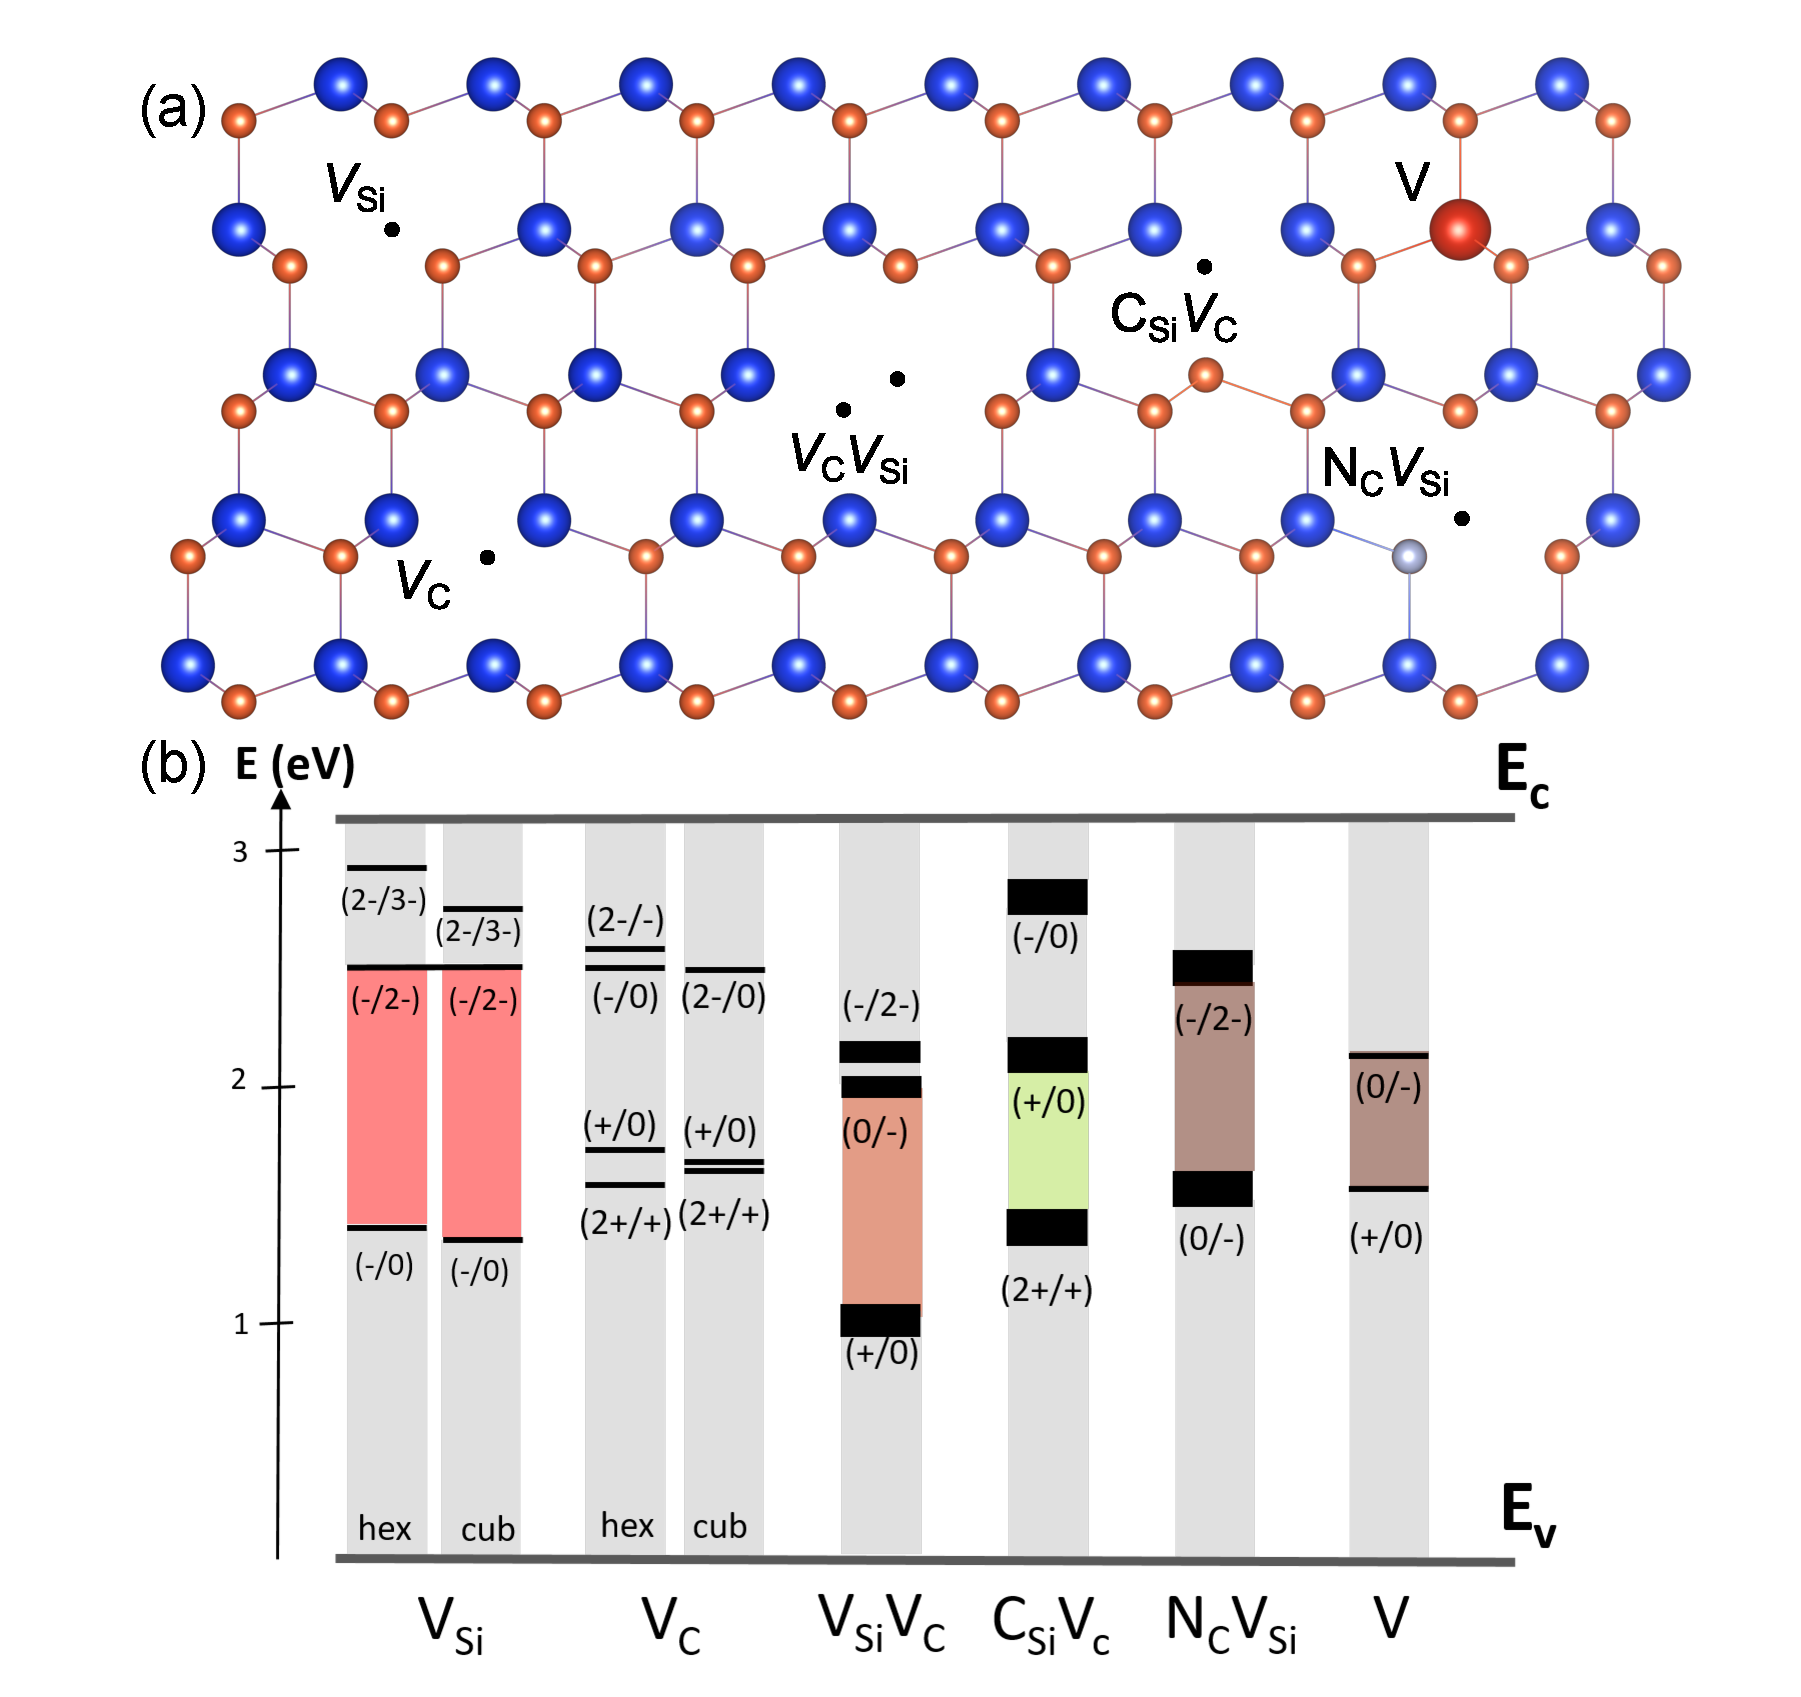
\includegraphics[width=0.5\textwidth]{figures/defects-sic.pdf}
 %   \caption{[PLACEHOLDER] Schematic representation of different quantum compatible defects in SiC and the energy levels they introduce into the band gap, from Ref.\cite{Bathen2021}.} 
 %   \label{fig:defects-sic}
%\end{figure}

%Table \ref{tab:qt-materials} contains an overview of known semiconductor materials with demonstrated quantum compatible characteristics. In this context we consider single-photon emission and coherent spin manipulation for systems related to point defects primarily, but also self-assembled or lithographically structured quantum dots. \marianne{A (placeholder) schematic of quantum compatible defects and the energy levels they introduce into the band gap of 4H-SiC is shown in Figure~\ref{fig:defects-sic}.} Most of the defects in the table have yet to be identified, and different material related challenges complicate the implementation of defects for QT. A set of common denominators for materials that contain qubit defects was summarized by Weber et al. \cite{Weber2010}: 
%\begin{itemize}
 %   \item Wide band gap to facilitate localized deep levels (physical)
 %    \item Low spin orbit coupling to extend spin coherence times (physical) 
 %   \item Low el-phonon coupling for sharp emission lines (physical) 
 %   \item Availability as high-quality, bulk, or thin-film single crystals (practical)
 %   \item Constituent elements with naturally occurring isotopes of zero nuclear spin (practical). 
%\end{itemize}
%Note the division between physical and practical requirements in the list above. The physical criteria refer to some fundamental aspect of the material that permits specific properties to manifest, while practical refers to the external influences that simplify measurement and detection of the interesting properties. In this work, we will focus primarily on the former set of criteria, as understanding them better may give further insights into the makings of a reliable QT platform. 

%In addition to obtaining greater understanding of  exactly what constitutes a good quantum host material, we must recognize that different defect and material types may suit different needs. Therefore, we aim to develop a bigger bank of candidate defects and materials. So far, detection of QT compatibility in semiconductors has been rather slow, depending on signal detection and later identification in each specific material. Instead, we are looking for a top-down approach to \textit{predict} promising materials, enabling a guiding of experimental efforts. 

%\subsection*{Density Functional Theory Output} %Marianne 
%The density functional theory (DFT) is a versatile and powerful theoretical approach that has been exceptionally successful in predicting solid-state material properties such as stability of different phases, lattice parameters and band gaps. DFT provides a method for iteratively solving the Schr{\"o}dinger equation based on initial guesses for the atomic potentials. Using DFT calculations, we are able to accurately investigate semiconductor materials with many atoms while keeping efficiency and cost in mind.  

%The fundamental challenge of the DFT is that the calculations rely on approximations to the potential function of a system as expressed by the exchange-correlation (XC) functional, which is not known for bulk materials. The XC functional is usually grouped into three categories based on the level of theory. The local density approximation (LDA) takes the homogeneous electron gas as a starting point, while the more advanced general gradient approximation (GGA) includes also the gradient in local electron gas variations. These local or semi-local functionals yield satisfactory results on geometrical concerns but tend to underestimate energies such as the band gap or defect energy levels due to a self-interaction error (i.e., an electron is allowed to interact with itself) [Ref SchollSteckel] \cite{Freysoldt2014}. More recent developments have seen the widespread use of hybrid functionals such as the HSE06 incorporating a portion of Hartree-Fock exact exchange \cite{Heyd2003},  albeit at a much greater computational cost. 

%Despite the limitations imposed by the approximate nature of the XC functional, and the band gap error of LDA and GGA level functionals, DFT can be a powerful tool when predicting, designing and interpreting experiments. Herein, we employ databases containing DFT calculations of material properties to gain insight into the fundamental mechanisms behind observed quantum characteristics, and predict new candidate QT hosts. The calculations we employ were performed using the GGA-level Perdew-Burke-Erznerhof (PBE) functional \cite{Perdew1996}. Note that the PBE functional tends to underestimate the band gap of semiconductor materials. Nonetheless, a larger data set is available than for, e.g., HSE06, and many trends are conserved also with PBE. The ground-state (and $0$~K) parameters that can be extracted from this type of data set include the total energy (translates into stability), the band gap, the electronegativity, the electron-phonon coupling and magnetic properties. 

%\begin{figure}[t]
%    \centering
%    \includegraphics[width=\textwidth]{figures/ht-workflow.jpg}
%    \caption{[PLACEHOLDER for workflow] Morten: can you please add the other schematic figure we discussed as placeholder? Sebastian makes our own versions of these schematic figures (I can make some VESTA files with materials). }
%    \label{fig:ht-workflow}
%\end{figure}

%\subsection*{Machine Learning} 

%Should contain a brief description of the four ``algorithms'':
%\begin{itemize}
 %   \item Logistic regression
 %   \item Decision trees
 %   \item Random forest
 %   \item Gradient boost
%\end{itemize}

%Why these? Works well out of the box, I guess. Readily available in scikit-learn.

\section*{Results and discussion}
%Includes discussion of results. 

\subsection*{Information Flow}  %Sebastian/Oliver (Marianne) 
% MEB: Since Methods are at the end, I propose to put part of this
% discussion in the Results section. 
% This is because it is an important result of the work, and also
% because it is important to understand the rest of the paper 

The information stream in this work can be regarded as many
modular parts connected in logical pieces. The initial step for
gathering material data and building features is visualized by the
the flowchart in Figure~\ref{fig:flowchart-makedata}. 
Initially, we start by extracting all entries in
the Materials Project that matches a specific query. 

\setlength{\abovecaptionskip}{5cm}
\begin{figure}[!ht]
\begin{picture}(20,10)

\setlength{\unitlength}{0.17in}
\put(-15,-5){\framebox(7,3){Initial MP query}}
\put(-8,-3.5){\vector(3,0){2}}
\put(-6,-3.5){\line(0,3){3}}
\put(-6,-3.5){\line(0,-3){3}}
\put(-6,-6.5){\line(1,0){17}}

\put(-1.5,-5){\framebox(3.5,2){AFLOW}}
\put(0.24,-5){\vector(0,-1){1.5}}

\put(3,-5){\framebox(5,2){AFLOW-ML}}
\put(5.5,-5){\vector(0,-1){1.5}}

\put(-3,-10){\framebox(3,2){OQMD}}
\put(-2.5,-8){\vector(0,1){1.5}}

\put(1,-10){\framebox(5,2){JARVIS-DFT}}
\put(3.5,-8){\vector(0,1){1.5}}

\put(7,-10){\framebox(2,2){CI}}
\put(8,-8){\vector(0,1){1.5}}

\put(-6,-0.5){\vector(1,0){5}}
\put(-1,-1.5){\framebox(8,2){Matminer featurizer}}
\put(7,-0.5){\line(1,0){4}}

\put(11,-0.5){\vector(0,-1){3}}
\put(11,-6.5){\vector(0,1){3}}

\put(11,-3.5){\vector(1,0){2}}
\put(13,-4.5){\framebox(6,2){interim data}}

\end{picture}
\caption{The data flow of the main project, starting from an initial MP-query, and ending with a featurized dataset with entries from several other databases. The matminer featurizer step is further visualized in-depth in Figure \ref{fig:flowchart-featurization}.}
\label{fig:flowchart-makedata}
\end{figure}
%\vskip0cm
%\setlength{\abovecaptionskip}{0cm}


\setlength{\abovecaptionskip}{10cm}
\begin{figure}[!ht]
\begin{picture}(20,20)
\setlength{\unitlength}{0.17in}

%\put(13.5, 0.5){\makebox{\thead{\textbf{Matminer featurizer}}}}
%\put(0.,-22){\framebox(33.5,22){\thead{}}}

\put(-16,-8.5){\vector(1,0){2.5}}
\put(-13.5,-10.5){\framebox(4,4){\thead{Partition \\ dataset}}}
\put(-9.5,-8.5){\vector(3,0){2}}
\put(-7.5,-10.5){\framebox(5,4){\thead{Get objects \\ from MP}}}
\put(-2.5,-8.5){\line(3,0){1}}
\put(-1.5,-8.5){\line(0,1){6}}
\put(-1.5,-8.5){\line(0,-1){6}}

\put(-1.5,-2.5){\vector(3,0){1}}
\put(-0.5,-3.5){\framebox(9,2){Featurize composition}}
\put(8.5,-2.5){\line(3,0){1}}

\put(-1.5,-5.5){\vector(3,0){1}}
\put(-0.5,-6.5){\framebox(9,2){Featurize structure}}
\put(8.5,-5.5){\line(3,0){1}}

\put(-1.5,-8.5){\vector(3,0){1}}
\put(-0.5,-9.5){\framebox(9,2){Featurize site}}
\put(8.5,-8.5){\line(3,0){1}}

\put(-1.5,-11.5){\vector(3,0){1}}
\put(-0.5,-12.5){\framebox(9,2){Featurize dos}}
\put(8.5,-11.5){\line(3,0){1}}

\put(-1.5,-14.5){\vector(3,0){1}}
\put(-0.5,-15.5){\framebox(9,2){Featurize band}}
\put(8.5,-14.5){\line(3,0){1}}

\put(9.5,-8.5){\line(0,1){6}}
\put(9.5,-8.5){\line(0,-1){6}}

\put(9.5,-8.5){\vector(2,0){1}}
\put(10.5,-10.5){\framebox(5.5,4){\thead{Done with \\ all partitions?}}}

\put(14, -12.){\makebox{NO}}
\put(13.5,-10.5){\line(0,-1){8}}
\put(13.5,-18.5){\vector(-1,0){16}}
\put(-7.5,-20.5){\framebox(5,4){\thead{Select next \\ partition}}}
\put(-5,-16.5){\vector(0,1){6}}


\put(16, -8.5){\vector(1,0){3.5}}
\put(16.5, -8.){\makebox{YES}}

\end{picture}
\caption{The process of the matminer featurizer step.  
%as seen in Figure \ref{fig:flowchart-makedata}. 
To limit the memory and computational usage, the data is partitioned into smaller subsets where the respective pymatgen objects are obtained through a query to be used in the following featurization steps. This process is repeated iteratively until all the data has been featurized. Abbreviations used are Materials Project (MP), density of states (DOS) and electronic band structure (band).}
\label{fig:flowchart-featurization}
\end{figure}
%\vskip15cm
%\setlength{\abovecaptionskip}{10cm}


Thereafter, we apply Matminer’s \cite{Ward2018}
featurization tools to make thousands of features of the data. The conditions for this initial query are that the materials must derive from experimental data, and have a band gap wider than $0.1$~eV. In a parallel step, entries that are deemed
similar to the entries from the initial query
are extracted from 
OQMD \cite{Saal2013,Kirklin2015}, JARVIS-DFT \cite{Choudhary2020}, 
AFLOW \cite{Curtarolo2012, Curtarolo2012a, Calderon2015}, 
AFLOW-ML \cite{Isayev2017},
and
Citrine Informatics REF!??. The results of these steps are combined into
a data set for further analysis.

A schematic describing the featurization process in Matminer is shown in Figure~\ref{fig:flowchart-featurization}. 
\textbf{[Describe it and say something about which features we choose.]}  
The 39 features selected in this work are summarized in the Supplementary Material at \cite{supplementary}. 


\subsection*{Data Mining}

After compiling a dataset from the procedure outlined above, we 
face a challenge in terms of defining a training set that %we can train data on. 
can be used to train an ML algorithm. 
This is challenging for two reasons. 
Firstly, although defects like the NV center in diamond and emitters in SiC are becoming
increasingly well studied, few candidate materials are known. An additional consideration
is that the physical mechanisms promoting favorable defect properties are not fully understood. 
Secondly, defining materials as unsuitable candidates for QT has proven to be surprisingly
intricate. 
%This is not only challenging due to the lack of known suitable candidates (1),  but also due to the intricacy of defining materials as unsuitable candidates (0). 
We follow three separate procedures to define a training set consisting of both suitable and unsuitable material candidates for QT. 

\subsubsection*{The Ferrenti approach}

The first approach to defining a training set is based on the criteria
from the paper by \citeauthor{Ferrenti2020} \cite{Ferrenti2020}.
They suggest a data mining process consisting of four stages by 
systematically evaluating the suitability of host materials from
the Materials Project. 

In this framework, we label \textbf{suitable} candidates by the following steps. 
\begin{enumerate}
    \item Include materials that;
    \begin{itemize}
        \item contain elements with more than $50\%$ natural abundance of 
            zero spin isotopes,
        \item crystallize in non-polar space groups,
        \item are present in the ICSD database, and
        \item are calculated to be nonmagnetic. 
    \end{itemize}
    \item Pragmatically remove toxic, radioactive and otherwise 
        ``difficult'' materials;
    \begin{itemize}
        \item exclude Th, U, Cd and Hg,
        \item exclude any rare-earth metals and noble gases,
        \item exclude Ru, Os, Fe or Ni.
    \end{itemize}
    \item Include only materials with a band gap larger than $0.5$~eV calculated using DFT and the PBE functional. 
    \item Ensure that energy above hull is less than $0.2$~eV per atom.
\end{enumerate}

We then label \textbf{unsuitable} candidates as materials in the ICSD database that crystallize in polar space groups, are calculated 
to be magnetic and have a band gap larger than $0.1$~eV as calculated by PBE-GGA.

\subsubsection*{The augmented Ferrenti approach}
In the second approach, we adjust the first approach in order to 
improve the dataset. This approach is therefore named
\emph{the augmented Ferrenti approach}.

In the first approach we included criteria that were not physically motivated, but instead based on a purely practical perspective, like excluding toxic and
radioactive elements. Such criteria are not necessarily related to what makes 
a material suitable for quantum technology - eventually it is up to the 
experimentalist to decide the practicality of the material to be employed. 
Consequently, in the augmented Ferrenti approach, we remove stage two from the approach above. What is more, we will include a few additional elements that have shown promising properties, but were initially excluded due to the lack of spin zero isotopes. 

The following steps make up the process of choosing \textbf{suitable} candidates 
in the \emph{augmented Ferrenti approach},
\begin{enumerate}
    \item Include materials that; 
    \begin{itemize}
        \item contain elements where more than half have a natural abundance of zero spin isotopes, except Al, P, Ga, As, B and N, 
        \item crystallize in non-polar space groups,
        \item are present in the ICSD database,
        \item are calculated to be nonmagnetic. 
    \end{itemize}
    \item Only keep materials that have a band gap larger than $1.5$~eV as calculated by PBE-GGA,
    \item Ensure energy above hull is less than $0.2$~eV per atom. 
\end{enumerate}

For \textbf{unsuitable} candidates, we implement the same strategy as the non-augmented
Ferrenti approach. The result is a somewhat unbalanced dataset, with up to $75 \ \%$ of the 
materials found in the suitable group. However, the dataset is $78 \ \%$ larger than for
the Ferrenti approach.

\subsubsection*{The insightful approach}
The third approach differs substantially from the first two approaches in terms 
of labeling, as we apply knowledge from the field (see for instance Refs.~\cite{Atatuere2018,Zhang2020,Son2020,Toth2019,Bathen2021} for an overview)   
to pick our promising material host candidates. We therefore name this scheme 
\emph{the insightful approach}. 
Due to the concern of having an insufficient dataset, we will include
materials that are promising and have shown suitable properties to 
accommodate deep defects that potentially can exhibit quantum effects. 
Materials where properties like single-photon emission and spin manipulation are attributed to quantum dot self-assembled formation or lithographic structuring will also be included in this context.  
The approach to pick \textbf{suitable} candidates can be summed up as;   
\begin{enumerate}
    \item Pick candidates that match the formulas in Table~\ref{tab:qt-materials}, or the formulas ZnSe,  AlP, GaP, AlAs, ZnTe, CdS \cite{Weber2010} or SiGe \cite{Hardy2019}. 
    \item Make sure the candidates are present in the ICSD database.  
    \item Perform a manual screening for correct structures.
\end{enumerate}

\begin{table}[b]
    \centering 
    \caption{Overview of materials and defects that have been demonstrated to exhibit QT compatible characteristics such as single-photon emission and coherent spin manipulation.}
    \begin{tabular}{c|c|c|c}
    Material & Band gap (eV) & Defect candidates & References \\
    \hline
    Diamond  & $5.5$  & N$_\mathrm{C}V_\mathrm{C}$, Si$_\mathrm{C}V_\mathrm{C}$, Ge$_\mathrm{C}V_\mathrm{C}$ & \cite{Taylor2008,Balasubramanian_2009,Barclay2011,Gordon2013,Rogers_2014,Bhaskar_2018} \\ 
    SiC & $2.2$-$3.3$ & $V_\mathrm{Si}$, $V_\mathrm{Si}V_\mathrm{C}$, C$_\mathrm{Si}V_\mathrm{C}$, N$_\mathrm{C}V_\mathrm{Si}$ & \cite{Widmann2014,Christle_2015,Castelletto_2014,Zargaleh_2018}  \cite{Weber2010, Son2020, Falk2013} \\ 
    Si & $1.1$ & P, G, unidentified & \cite{Muhonen_2014,Durand_2020,Redjem2020} \\ 
    (2D) \textit{h}-BN & $6.0$ & Unidentified defects & \cite{Tran_2016,Tran_2016b,Hayee_2020} \\ 
    (2D) MoS$_2$, WSe$_2$, WS$_2$ & $<2.5$~eV & Bound excitons & \cite{Toth2019} \\
    ZnO & $3.4$ & Unidentified defects & \cite{Morfa2012} \\ 
    ZnS & $3.6$ (zincblende) & Unidentified defects & \cite{Stewart2019} \\ 
    GaAs & $1.4$ & Quantum dots & \cite{Bluhm2010} \\ 
    GaN & $3.4$ & Quantum dots, unidentified defects & \cite{Roux2017,Berhane2018} \\
    AlN & $6.0$ & Unidentified defects & \cite{Xue2020}\\
    \end{tabular}
    \label{tab:qt-materials}
\end{table} 

Table~\ref{tab:qt-materials} contains an overview of known semiconductor materials with demonstrated quantum compatible characteristics. In this context, we consider single-photon emission and coherent spin manipulation.   
The table forms the basis for picking suitable candidates for the insightful approach. 
The properties being studied arise from mechanisms related to, e.g., point defects, excitons, and both self-assembled and lithographically structures quantum dots. 
Quantum emission signatures have been assigned to specific defects in diamond and SiC, but for most other materials, identification of the responsible defects still remains. 
In the insightful approach, we include materials that are known to be quantum compatible as outlined in Table~\ref{tab:qt-materials} in the training set, but also the materials ZnSe, AlP, GaP, AlAs, ZnTe, CdS and SiGe that have been predicted to act as good quantum hosts based on favorable properties such as wide band gap and low spin-orbit coupling \cite{Weber2010,Hardy2019}. 

After the first stage of picking candidates we are left with a list of 202 matching formulas which include 12 entries that have a band gap of less than $0.4$~eV. These structures are unstable in terms of energy above hull calculations, and will decompose into other materials in the list with a band gap that is substantially above $0.5$~eV. We include all of these structures except for C (mp-568410) having a PBE-computed band gap of $0.12$~eV - a metal according to AFLOW-ML and therefore labeled as an unsuitable candidate. 
 
%% OH: Dirty details about suitable materials:
Entries matching the formula C, SiC, BN, MoS$_2$, WSe$_2$ and WS$_2$ were manually screened to see if the entries have a matching structure to the respective candidates discussed earlier. %OH: Is discussed earlier in thesis but maybe neccessary to mention here? 
For C, we admit three-dimensional diamond-like structures as explicitly stated in the column tags at Materials Project. Additionally, we find many two-dimensional structures of carbon with a large band gap ($>1.5$ eV) in the data. We add these as suitable candidates. Complex structures (eg. C$_{28}$, C$_{48}$, C$_{60}$) were moved to the test set. For SiC, we admitted all entries, which involved $2$H, $3$C, $4$H, $6$H and $15$R. Concerning BN, MoS$_2$, WSe$_2$ and  WS$_2$, we only admit two-dimensional structures. For non-matching structures not mentioned so far, we move them to the test set to see if they will be predicted suitable or not by the models in a later step.

The materials AlP, GaP, AlAs, ZnTe and CdS were manually screened for tetrahedrally coordinated structures, and have been included since \citeauthor{Weber2010} \cite{Weber2010} has identified them as potentially promising candidates due to acceptable properties defined in requirements (H1-H4) in \autoref{ssec:qubit-material-host-requirements}. We note that only tetrahedrally coordinated structures of the given formulas were present after the band gap restriction of $0.5eV$.

The suitable candidates contain only compounds that are either elementary (unary) or binary. We do not want to discriminate based on the number of elements in a compound, therefore we remove the feature that describes the number of elements in a compound. After three stages, a total of $187$ entries were labeled as suitable candidates.
%% OH: Stop details suitable materials

Since the dataset constituting suitable candidates in the third approach contains few entries, we add 400 \emph{unsuitable}
candidates. These are picked at random from the pool of unsuitable candidates 
from the two previous approaches, in addition to those that are marked as unsuitable through
the manual screening process. 
See the Supplementary Material at \cite{supplementary} for a table containing the manually screened materials that were labeled as suitable candidates in the training set for the insightful approach. 


\subsubsection*{Comparing the approaches}

The three different methods for data mining place a particular emphasis on each of their particular goals. The Ferrenti approach depends on choosing only elements with zero spin isotopes together with practical filters, while the augmented Ferrenti approach allows a larger variety of elements and removes the practical reasons for excluding elements. Thus, the first approach targets a more narrow prediction space than the second approach does. However, perhaps the most restricted approach is the insightful approach. Since the variety of known suitable materials is substantially more restricted than for the two other approaches, we would expect the insightful approach to provide an even narrower prediction space. 
\textbf{[Are there any pros or cons we could mention on narrow prediction spaces?]}

%\marianne{Short paragraph here (or somewhere else) highlighting the potential issues with the two first approaches in terms of actually identifying any trends.}

We provide a visualization of each approach's training data as a parallel coordinate plot for a few selected features in Figure~\ref{fig:parallel-coordinates-approaches}. Parallel coordinate schemes \cite{Inselberga1990, Inselberg1985} represent a multi-dimensional data tuple as one polyline crossing a parallel axis. The selected features are found on the x-axis, while the y-axis shows the value of the data present. Thus, parallel coordinate plots can turn many-dimensional data into a compact two-dimensional representation. Due to possible data cluttering, the figure visualizes a random sample of each class with an upper limit of $250$ per class with transparent lines. The green and red polylines represent suitable and unsuitable candidates, respectively. 

The Ferrenti approach and the augmented Ferrenti approach share similarities; 
for example, all unsuitable candidates exhibit polar space groups, and their upper limits for both ionic character and covalent range are equal for suitable candidates.  
%such as having only unsuitable candidates with polar space groups and having an equal amount of upper limit for both ionic character and covalent range for suitable characters. 
Additionally, the two approaches share that suitable candidates can consist of up to five different elements. 
Interestingly, we observe that
the entries in Fig.~\ref{fig:parallel-coordinates-approaches} span the same dimensions for the Ferrenti and augmented Ferrenti approaches, despite the more restricted nature of the former. 
%even if the augmented Ferrenti approach is less restricted, it appears that the entries span the same dimensions.

The biggest difference is found for the insightful approach. The entries selected as suitable candidates do not exhibit any magnetization, even though there are both polar and non-polar space groups present. Additionally, the range of covalent radius and maximum ionic character span a substantially smaller space than the Ferrenti-based approaches. 
\textbf{This can be interpreted as ... }

\begin{figure}[t] %!htp
    \centering
    \begin{subfigure}{1\textwidth}
        \centering
          %% Creator: Matplotlib, PGF backend
%%
%% To include the figure in your LaTeX document, write
%%   \input{<filename>.pgf}
%%
%% Make sure the required packages are loaded in your preamble
%%   \usepackage{pgf}
%%
%% Also ensure that all the required font packages are loaded; for instance,
%% the lmodern package is sometimes necessary when using math font.
%%   \usepackage{lmodern}
%%
%% Figures using additional raster images can only be included by \input if
%% they are in the same directory as the main LaTeX file. For loading figures
%% from other directories you can use the `import` package
%%   \usepackage{import}
%%
%% and then include the figures with
%%   \import{<path to file>}{<filename>.pgf}
%%
%% Matplotlib used the following preamble
%%   \usepackage[detect-all,locale=DE]{siunitx} \usepackage[T1]{fontenc} \usepackage[utf8x]{inputenc}
%%
\begingroup%
\makeatletter%
\begin{pgfpicture}%
\pgfpathrectangle{\pgfpointorigin}{\pgfqpoint{3.879801in}{3.778301in}}%
\pgfusepath{use as bounding box, clip}%
\begin{pgfscope}%
\pgfsetbuttcap%
\pgfsetmiterjoin%
\pgfsetlinewidth{0.000000pt}%
\definecolor{currentstroke}{rgb}{1.000000,1.000000,1.000000}%
\pgfsetstrokecolor{currentstroke}%
\pgfsetstrokeopacity{0.000000}%
\pgfsetdash{}{0pt}%
\pgfpathmoveto{\pgfqpoint{0.000000in}{0.000000in}}%
\pgfpathlineto{\pgfqpoint{3.879801in}{0.000000in}}%
\pgfpathlineto{\pgfqpoint{3.879801in}{3.778301in}}%
\pgfpathlineto{\pgfqpoint{0.000000in}{3.778301in}}%
\pgfpathlineto{\pgfqpoint{0.000000in}{0.000000in}}%
\pgfpathclose%
\pgfusepath{}%
\end{pgfscope}%
\begin{pgfscope}%
\pgfsetbuttcap%
\pgfsetmiterjoin%
\definecolor{currentfill}{rgb}{1.000000,1.000000,1.000000}%
\pgfsetfillcolor{currentfill}%
\pgfsetlinewidth{0.000000pt}%
\definecolor{currentstroke}{rgb}{0.000000,0.000000,0.000000}%
\pgfsetstrokecolor{currentstroke}%
\pgfsetstrokeopacity{0.000000}%
\pgfsetdash{}{0pt}%
\pgfpathmoveto{\pgfqpoint{0.618106in}{0.473557in}}%
\pgfpathlineto{\pgfqpoint{3.704375in}{0.473557in}}%
\pgfpathlineto{\pgfqpoint{3.704375in}{3.480181in}}%
\pgfpathlineto{\pgfqpoint{0.618106in}{3.480181in}}%
\pgfpathlineto{\pgfqpoint{0.618106in}{0.473557in}}%
\pgfpathclose%
\pgfusepath{fill}%
\end{pgfscope}%
\begin{pgfscope}%
\pgfpathrectangle{\pgfqpoint{0.618106in}{0.473557in}}{\pgfqpoint{3.086269in}{3.006623in}}%
\pgfusepath{clip}%
\pgfsetbuttcap%
\pgfsetroundjoin%
\definecolor{currentfill}{rgb}{1.000000,0.647059,0.000000}%
\pgfsetfillcolor{currentfill}%
\pgfsetlinewidth{1.505625pt}%
\definecolor{currentstroke}{rgb}{1.000000,0.647059,0.000000}%
\pgfsetstrokecolor{currentstroke}%
\pgfsetdash{}{0pt}%
\pgfsys@defobject{currentmarker}{\pgfqpoint{-0.031056in}{-0.031056in}}{\pgfqpoint{0.031056in}{0.031056in}}{%
\pgfpathmoveto{\pgfqpoint{-0.031056in}{-0.031056in}}%
\pgfpathlineto{\pgfqpoint{0.031056in}{0.031056in}}%
\pgfpathmoveto{\pgfqpoint{-0.031056in}{0.031056in}}%
\pgfpathlineto{\pgfqpoint{0.031056in}{-0.031056in}}%
\pgfusepath{stroke,fill}%
}%
\end{pgfscope}%
\begin{pgfscope}%
\pgfpathrectangle{\pgfqpoint{0.618106in}{0.473557in}}{\pgfqpoint{3.086269in}{3.006623in}}%
\pgfusepath{clip}%
\pgfsetbuttcap%
\pgfsetroundjoin%
\definecolor{currentfill}{rgb}{0.000000,0.000000,0.000000}%
\pgfsetfillcolor{currentfill}%
\pgfsetlinewidth{1.505625pt}%
\definecolor{currentstroke}{rgb}{0.000000,0.000000,0.000000}%
\pgfsetstrokecolor{currentstroke}%
\pgfsetdash{}{0pt}%
\pgfsys@defobject{currentmarker}{\pgfqpoint{-0.031056in}{-0.031056in}}{\pgfqpoint{0.031056in}{0.031056in}}{%
\pgfpathmoveto{\pgfqpoint{-0.031056in}{0.000000in}}%
\pgfpathlineto{\pgfqpoint{0.031056in}{0.000000in}}%
\pgfpathmoveto{\pgfqpoint{0.000000in}{-0.031056in}}%
\pgfpathlineto{\pgfqpoint{0.000000in}{0.031056in}}%
\pgfusepath{stroke,fill}%
}%
\end{pgfscope}%
\begin{pgfscope}%
\pgfpathrectangle{\pgfqpoint{0.618106in}{0.473557in}}{\pgfqpoint{3.086269in}{3.006623in}}%
\pgfusepath{clip}%
\pgfsetbuttcap%
\pgfsetroundjoin%
\definecolor{currentfill}{rgb}{0.000000,0.000000,1.000000}%
\pgfsetfillcolor{currentfill}%
\pgfsetlinewidth{1.003750pt}%
\definecolor{currentstroke}{rgb}{0.000000,0.000000,1.000000}%
\pgfsetstrokecolor{currentstroke}%
\pgfsetdash{}{0pt}%
\pgfsys@defobject{currentmarker}{\pgfqpoint{-0.029536in}{-0.025125in}}{\pgfqpoint{0.029536in}{0.031056in}}{%
\pgfpathmoveto{\pgfqpoint{0.000000in}{0.031056in}}%
\pgfpathlineto{\pgfqpoint{-0.006973in}{0.009597in}}%
\pgfpathlineto{\pgfqpoint{-0.029536in}{0.009597in}}%
\pgfpathlineto{\pgfqpoint{-0.011282in}{-0.003666in}}%
\pgfpathlineto{\pgfqpoint{-0.018255in}{-0.025125in}}%
\pgfpathlineto{\pgfqpoint{-0.000000in}{-0.011863in}}%
\pgfpathlineto{\pgfqpoint{0.018255in}{-0.025125in}}%
\pgfpathlineto{\pgfqpoint{0.011282in}{-0.003666in}}%
\pgfpathlineto{\pgfqpoint{0.029536in}{0.009597in}}%
\pgfpathlineto{\pgfqpoint{0.006973in}{0.009597in}}%
\pgfpathlineto{\pgfqpoint{0.000000in}{0.031056in}}%
\pgfpathclose%
\pgfusepath{stroke,fill}%
}%
\end{pgfscope}%
\begin{pgfscope}%
\pgfpathrectangle{\pgfqpoint{0.618106in}{0.473557in}}{\pgfqpoint{3.086269in}{3.006623in}}%
\pgfusepath{clip}%
\pgfsetbuttcap%
\pgfsetroundjoin%
\definecolor{currentfill}{rgb}{0.196078,0.803922,0.196078}%
\pgfsetfillcolor{currentfill}%
\pgfsetlinewidth{1.003750pt}%
\definecolor{currentstroke}{rgb}{0.196078,0.803922,0.196078}%
\pgfsetstrokecolor{currentstroke}%
\pgfsetdash{}{0pt}%
\pgfsys@defobject{currentmarker}{\pgfqpoint{-0.031056in}{-0.031056in}}{\pgfqpoint{0.031056in}{0.031056in}}{%
\pgfpathmoveto{\pgfqpoint{-0.031056in}{-0.031056in}}%
\pgfpathlineto{\pgfqpoint{0.031056in}{-0.031056in}}%
\pgfpathlineto{\pgfqpoint{0.031056in}{0.031056in}}%
\pgfpathlineto{\pgfqpoint{-0.031056in}{0.031056in}}%
\pgfpathlineto{\pgfqpoint{-0.031056in}{-0.031056in}}%
\pgfpathclose%
\pgfusepath{stroke,fill}%
}%
\begin{pgfscope}%
\pgfsys@transformshift{1.915552in}{3.293752in}%
\pgfsys@useobject{currentmarker}{}%
\end{pgfscope}%
\begin{pgfscope}%
\pgfsys@transformshift{1.557757in}{3.282052in}%
\pgfsys@useobject{currentmarker}{}%
\end{pgfscope}%
\begin{pgfscope}%
\pgfsys@transformshift{1.288549in}{3.349375in}%
\pgfsys@useobject{currentmarker}{}%
\end{pgfscope}%
\begin{pgfscope}%
\pgfsys@transformshift{2.230607in}{2.385818in}%
\pgfsys@useobject{currentmarker}{}%
\end{pgfscope}%
\begin{pgfscope}%
\pgfsys@transformshift{2.230452in}{2.376003in}%
\pgfsys@useobject{currentmarker}{}%
\end{pgfscope}%
\begin{pgfscope}%
\pgfsys@transformshift{2.169621in}{3.347236in}%
\pgfsys@useobject{currentmarker}{}%
\end{pgfscope}%
\begin{pgfscope}%
\pgfsys@transformshift{2.167488in}{3.192471in}%
\pgfsys@useobject{currentmarker}{}%
\end{pgfscope}%
\begin{pgfscope}%
\pgfsys@transformshift{2.190888in}{3.342759in}%
\pgfsys@useobject{currentmarker}{}%
\end{pgfscope}%
\begin{pgfscope}%
\pgfsys@transformshift{1.591135in}{3.294704in}%
\pgfsys@useobject{currentmarker}{}%
\end{pgfscope}%
\begin{pgfscope}%
\pgfsys@transformshift{1.593842in}{3.041748in}%
\pgfsys@useobject{currentmarker}{}%
\end{pgfscope}%
\begin{pgfscope}%
\pgfsys@transformshift{1.593867in}{3.092916in}%
\pgfsys@useobject{currentmarker}{}%
\end{pgfscope}%
\begin{pgfscope}%
\pgfsys@transformshift{2.319005in}{2.966009in}%
\pgfsys@useobject{currentmarker}{}%
\end{pgfscope}%
\begin{pgfscope}%
\pgfsys@transformshift{2.288015in}{2.260826in}%
\pgfsys@useobject{currentmarker}{}%
\end{pgfscope}%
\begin{pgfscope}%
\pgfsys@transformshift{1.773186in}{2.115878in}%
\pgfsys@useobject{currentmarker}{}%
\end{pgfscope}%
\begin{pgfscope}%
\pgfsys@transformshift{1.650455in}{2.007670in}%
\pgfsys@useobject{currentmarker}{}%
\end{pgfscope}%
\begin{pgfscope}%
\pgfsys@transformshift{1.906194in}{1.397513in}%
\pgfsys@useobject{currentmarker}{}%
\end{pgfscope}%
\begin{pgfscope}%
\pgfsys@transformshift{2.031167in}{1.817281in}%
\pgfsys@useobject{currentmarker}{}%
\end{pgfscope}%
\begin{pgfscope}%
\pgfsys@transformshift{2.087020in}{1.416206in}%
\pgfsys@useobject{currentmarker}{}%
\end{pgfscope}%
\begin{pgfscope}%
\pgfsys@transformshift{1.960772in}{1.718309in}%
\pgfsys@useobject{currentmarker}{}%
\end{pgfscope}%
\begin{pgfscope}%
\pgfsys@transformshift{1.947251in}{2.143412in}%
\pgfsys@useobject{currentmarker}{}%
\end{pgfscope}%
\begin{pgfscope}%
\pgfsys@transformshift{1.482040in}{2.435199in}%
\pgfsys@useobject{currentmarker}{}%
\end{pgfscope}%
\begin{pgfscope}%
\pgfsys@transformshift{1.820591in}{1.867241in}%
\pgfsys@useobject{currentmarker}{}%
\end{pgfscope}%
\begin{pgfscope}%
\pgfsys@transformshift{1.541486in}{2.588881in}%
\pgfsys@useobject{currentmarker}{}%
\end{pgfscope}%
\begin{pgfscope}%
\pgfsys@transformshift{1.657475in}{2.232288in}%
\pgfsys@useobject{currentmarker}{}%
\end{pgfscope}%
\begin{pgfscope}%
\pgfsys@transformshift{1.428807in}{2.584899in}%
\pgfsys@useobject{currentmarker}{}%
\end{pgfscope}%
\begin{pgfscope}%
\pgfsys@transformshift{1.767168in}{1.601983in}%
\pgfsys@useobject{currentmarker}{}%
\end{pgfscope}%
\begin{pgfscope}%
\pgfsys@transformshift{1.537158in}{2.542407in}%
\pgfsys@useobject{currentmarker}{}%
\end{pgfscope}%
\begin{pgfscope}%
\pgfsys@transformshift{2.151064in}{2.305778in}%
\pgfsys@useobject{currentmarker}{}%
\end{pgfscope}%
\begin{pgfscope}%
\pgfsys@transformshift{2.245598in}{2.239982in}%
\pgfsys@useobject{currentmarker}{}%
\end{pgfscope}%
\begin{pgfscope}%
\pgfsys@transformshift{1.792253in}{1.258886in}%
\pgfsys@useobject{currentmarker}{}%
\end{pgfscope}%
\begin{pgfscope}%
\pgfsys@transformshift{1.724865in}{2.267079in}%
\pgfsys@useobject{currentmarker}{}%
\end{pgfscope}%
\begin{pgfscope}%
\pgfsys@transformshift{1.787183in}{1.802827in}%
\pgfsys@useobject{currentmarker}{}%
\end{pgfscope}%
\begin{pgfscope}%
\pgfsys@transformshift{2.026675in}{1.967225in}%
\pgfsys@useobject{currentmarker}{}%
\end{pgfscope}%
\begin{pgfscope}%
\pgfsys@transformshift{1.875597in}{1.393118in}%
\pgfsys@useobject{currentmarker}{}%
\end{pgfscope}%
\begin{pgfscope}%
\pgfsys@transformshift{0.940489in}{2.715813in}%
\pgfsys@useobject{currentmarker}{}%
\end{pgfscope}%
\begin{pgfscope}%
\pgfsys@transformshift{1.197317in}{2.393296in}%
\pgfsys@useobject{currentmarker}{}%
\end{pgfscope}%
\begin{pgfscope}%
\pgfsys@transformshift{1.681884in}{1.766591in}%
\pgfsys@useobject{currentmarker}{}%
\end{pgfscope}%
\begin{pgfscope}%
\pgfsys@transformshift{1.563376in}{2.395138in}%
\pgfsys@useobject{currentmarker}{}%
\end{pgfscope}%
\begin{pgfscope}%
\pgfsys@transformshift{1.740306in}{2.481149in}%
\pgfsys@useobject{currentmarker}{}%
\end{pgfscope}%
\begin{pgfscope}%
\pgfsys@transformshift{1.760363in}{2.272624in}%
\pgfsys@useobject{currentmarker}{}%
\end{pgfscope}%
\begin{pgfscope}%
\pgfsys@transformshift{1.436507in}{2.696115in}%
\pgfsys@useobject{currentmarker}{}%
\end{pgfscope}%
\begin{pgfscope}%
\pgfsys@transformshift{1.006935in}{2.452925in}%
\pgfsys@useobject{currentmarker}{}%
\end{pgfscope}%
\begin{pgfscope}%
\pgfsys@transformshift{1.574497in}{1.868790in}%
\pgfsys@useobject{currentmarker}{}%
\end{pgfscope}%
\begin{pgfscope}%
\pgfsys@transformshift{1.776300in}{1.594829in}%
\pgfsys@useobject{currentmarker}{}%
\end{pgfscope}%
\begin{pgfscope}%
\pgfsys@transformshift{1.357499in}{2.337319in}%
\pgfsys@useobject{currentmarker}{}%
\end{pgfscope}%
\begin{pgfscope}%
\pgfsys@transformshift{1.252428in}{1.987776in}%
\pgfsys@useobject{currentmarker}{}%
\end{pgfscope}%
\begin{pgfscope}%
\pgfsys@transformshift{1.542556in}{2.623552in}%
\pgfsys@useobject{currentmarker}{}%
\end{pgfscope}%
\begin{pgfscope}%
\pgfsys@transformshift{1.130836in}{2.419789in}%
\pgfsys@useobject{currentmarker}{}%
\end{pgfscope}%
\begin{pgfscope}%
\pgfsys@transformshift{2.051213in}{1.633134in}%
\pgfsys@useobject{currentmarker}{}%
\end{pgfscope}%
\begin{pgfscope}%
\pgfsys@transformshift{1.699953in}{2.157893in}%
\pgfsys@useobject{currentmarker}{}%
\end{pgfscope}%
\begin{pgfscope}%
\pgfsys@transformshift{1.141327in}{2.374297in}%
\pgfsys@useobject{currentmarker}{}%
\end{pgfscope}%
\begin{pgfscope}%
\pgfsys@transformshift{1.701659in}{2.245890in}%
\pgfsys@useobject{currentmarker}{}%
\end{pgfscope}%
\begin{pgfscope}%
\pgfsys@transformshift{1.065207in}{2.582958in}%
\pgfsys@useobject{currentmarker}{}%
\end{pgfscope}%
\begin{pgfscope}%
\pgfsys@transformshift{1.780533in}{1.662057in}%
\pgfsys@useobject{currentmarker}{}%
\end{pgfscope}%
\begin{pgfscope}%
\pgfsys@transformshift{1.976368in}{1.820615in}%
\pgfsys@useobject{currentmarker}{}%
\end{pgfscope}%
\begin{pgfscope}%
\pgfsys@transformshift{2.158742in}{2.719967in}%
\pgfsys@useobject{currentmarker}{}%
\end{pgfscope}%
\begin{pgfscope}%
\pgfsys@transformshift{1.710344in}{2.290945in}%
\pgfsys@useobject{currentmarker}{}%
\end{pgfscope}%
\begin{pgfscope}%
\pgfsys@transformshift{1.261145in}{2.329795in}%
\pgfsys@useobject{currentmarker}{}%
\end{pgfscope}%
\begin{pgfscope}%
\pgfsys@transformshift{1.743844in}{2.229781in}%
\pgfsys@useobject{currentmarker}{}%
\end{pgfscope}%
\begin{pgfscope}%
\pgfsys@transformshift{1.743123in}{2.022913in}%
\pgfsys@useobject{currentmarker}{}%
\end{pgfscope}%
\begin{pgfscope}%
\pgfsys@transformshift{1.642283in}{2.261926in}%
\pgfsys@useobject{currentmarker}{}%
\end{pgfscope}%
\begin{pgfscope}%
\pgfsys@transformshift{2.099484in}{1.598112in}%
\pgfsys@useobject{currentmarker}{}%
\end{pgfscope}%
\begin{pgfscope}%
\pgfsys@transformshift{1.889869in}{1.275311in}%
\pgfsys@useobject{currentmarker}{}%
\end{pgfscope}%
\begin{pgfscope}%
\pgfsys@transformshift{1.152832in}{2.559825in}%
\pgfsys@useobject{currentmarker}{}%
\end{pgfscope}%
\begin{pgfscope}%
\pgfsys@transformshift{1.030564in}{2.967384in}%
\pgfsys@useobject{currentmarker}{}%
\end{pgfscope}%
\begin{pgfscope}%
\pgfsys@transformshift{1.601268in}{2.081533in}%
\pgfsys@useobject{currentmarker}{}%
\end{pgfscope}%
\begin{pgfscope}%
\pgfsys@transformshift{0.968699in}{2.663683in}%
\pgfsys@useobject{currentmarker}{}%
\end{pgfscope}%
\begin{pgfscope}%
\pgfsys@transformshift{1.679785in}{2.096384in}%
\pgfsys@useobject{currentmarker}{}%
\end{pgfscope}%
\begin{pgfscope}%
\pgfsys@transformshift{1.745272in}{2.163268in}%
\pgfsys@useobject{currentmarker}{}%
\end{pgfscope}%
\begin{pgfscope}%
\pgfsys@transformshift{2.068323in}{2.082699in}%
\pgfsys@useobject{currentmarker}{}%
\end{pgfscope}%
\begin{pgfscope}%
\pgfsys@transformshift{1.519213in}{2.212313in}%
\pgfsys@useobject{currentmarker}{}%
\end{pgfscope}%
\begin{pgfscope}%
\pgfsys@transformshift{1.402247in}{2.624348in}%
\pgfsys@useobject{currentmarker}{}%
\end{pgfscope}%
\begin{pgfscope}%
\pgfsys@transformshift{1.388212in}{2.895494in}%
\pgfsys@useobject{currentmarker}{}%
\end{pgfscope}%
\begin{pgfscope}%
\pgfsys@transformshift{1.042954in}{2.719209in}%
\pgfsys@useobject{currentmarker}{}%
\end{pgfscope}%
\begin{pgfscope}%
\pgfsys@transformshift{1.452084in}{1.952726in}%
\pgfsys@useobject{currentmarker}{}%
\end{pgfscope}%
\begin{pgfscope}%
\pgfsys@transformshift{1.510973in}{2.445200in}%
\pgfsys@useobject{currentmarker}{}%
\end{pgfscope}%
\begin{pgfscope}%
\pgfsys@transformshift{1.619529in}{2.458431in}%
\pgfsys@useobject{currentmarker}{}%
\end{pgfscope}%
\begin{pgfscope}%
\pgfsys@transformshift{1.300375in}{1.936566in}%
\pgfsys@useobject{currentmarker}{}%
\end{pgfscope}%
\begin{pgfscope}%
\pgfsys@transformshift{1.815717in}{2.005290in}%
\pgfsys@useobject{currentmarker}{}%
\end{pgfscope}%
\begin{pgfscope}%
\pgfsys@transformshift{1.991364in}{2.099340in}%
\pgfsys@useobject{currentmarker}{}%
\end{pgfscope}%
\begin{pgfscope}%
\pgfsys@transformshift{1.864874in}{1.662419in}%
\pgfsys@useobject{currentmarker}{}%
\end{pgfscope}%
\begin{pgfscope}%
\pgfsys@transformshift{2.008700in}{1.721579in}%
\pgfsys@useobject{currentmarker}{}%
\end{pgfscope}%
\begin{pgfscope}%
\pgfsys@transformshift{1.071661in}{2.624603in}%
\pgfsys@useobject{currentmarker}{}%
\end{pgfscope}%
\begin{pgfscope}%
\pgfsys@transformshift{1.438546in}{2.310375in}%
\pgfsys@useobject{currentmarker}{}%
\end{pgfscope}%
\begin{pgfscope}%
\pgfsys@transformshift{1.469214in}{1.947322in}%
\pgfsys@useobject{currentmarker}{}%
\end{pgfscope}%
\begin{pgfscope}%
\pgfsys@transformshift{1.087238in}{2.808672in}%
\pgfsys@useobject{currentmarker}{}%
\end{pgfscope}%
\begin{pgfscope}%
\pgfsys@transformshift{1.761682in}{1.956658in}%
\pgfsys@useobject{currentmarker}{}%
\end{pgfscope}%
\begin{pgfscope}%
\pgfsys@transformshift{1.970999in}{1.621858in}%
\pgfsys@useobject{currentmarker}{}%
\end{pgfscope}%
\begin{pgfscope}%
\pgfsys@transformshift{1.099958in}{2.781599in}%
\pgfsys@useobject{currentmarker}{}%
\end{pgfscope}%
\begin{pgfscope}%
\pgfsys@transformshift{1.728844in}{1.748634in}%
\pgfsys@useobject{currentmarker}{}%
\end{pgfscope}%
\begin{pgfscope}%
\pgfsys@transformshift{1.947337in}{2.145058in}%
\pgfsys@useobject{currentmarker}{}%
\end{pgfscope}%
\begin{pgfscope}%
\pgfsys@transformshift{1.074418in}{2.490941in}%
\pgfsys@useobject{currentmarker}{}%
\end{pgfscope}%
\begin{pgfscope}%
\pgfsys@transformshift{1.886016in}{2.210784in}%
\pgfsys@useobject{currentmarker}{}%
\end{pgfscope}%
\begin{pgfscope}%
\pgfsys@transformshift{2.022582in}{1.509026in}%
\pgfsys@useobject{currentmarker}{}%
\end{pgfscope}%
\begin{pgfscope}%
\pgfsys@transformshift{1.801289in}{1.252059in}%
\pgfsys@useobject{currentmarker}{}%
\end{pgfscope}%
\begin{pgfscope}%
\pgfsys@transformshift{2.213113in}{1.557586in}%
\pgfsys@useobject{currentmarker}{}%
\end{pgfscope}%
\begin{pgfscope}%
\pgfsys@transformshift{2.357097in}{1.622057in}%
\pgfsys@useobject{currentmarker}{}%
\end{pgfscope}%
\begin{pgfscope}%
\pgfsys@transformshift{1.722638in}{1.389779in}%
\pgfsys@useobject{currentmarker}{}%
\end{pgfscope}%
\begin{pgfscope}%
\pgfsys@transformshift{2.397661in}{1.718134in}%
\pgfsys@useobject{currentmarker}{}%
\end{pgfscope}%
\begin{pgfscope}%
\pgfsys@transformshift{1.982528in}{1.371568in}%
\pgfsys@useobject{currentmarker}{}%
\end{pgfscope}%
\begin{pgfscope}%
\pgfsys@transformshift{2.141835in}{1.534803in}%
\pgfsys@useobject{currentmarker}{}%
\end{pgfscope}%
\begin{pgfscope}%
\pgfsys@transformshift{2.451532in}{1.924030in}%
\pgfsys@useobject{currentmarker}{}%
\end{pgfscope}%
\begin{pgfscope}%
\pgfsys@transformshift{2.041041in}{1.629933in}%
\pgfsys@useobject{currentmarker}{}%
\end{pgfscope}%
\begin{pgfscope}%
\pgfsys@transformshift{2.238412in}{1.523200in}%
\pgfsys@useobject{currentmarker}{}%
\end{pgfscope}%
\begin{pgfscope}%
\pgfsys@transformshift{2.193723in}{1.244457in}%
\pgfsys@useobject{currentmarker}{}%
\end{pgfscope}%
\begin{pgfscope}%
\pgfsys@transformshift{2.289748in}{1.367862in}%
\pgfsys@useobject{currentmarker}{}%
\end{pgfscope}%
\begin{pgfscope}%
\pgfsys@transformshift{2.009012in}{1.448848in}%
\pgfsys@useobject{currentmarker}{}%
\end{pgfscope}%
\begin{pgfscope}%
\pgfsys@transformshift{2.134214in}{1.667067in}%
\pgfsys@useobject{currentmarker}{}%
\end{pgfscope}%
\begin{pgfscope}%
\pgfsys@transformshift{1.711342in}{1.474019in}%
\pgfsys@useobject{currentmarker}{}%
\end{pgfscope}%
\begin{pgfscope}%
\pgfsys@transformshift{1.929953in}{1.303291in}%
\pgfsys@useobject{currentmarker}{}%
\end{pgfscope}%
\begin{pgfscope}%
\pgfsys@transformshift{1.754882in}{1.478721in}%
\pgfsys@useobject{currentmarker}{}%
\end{pgfscope}%
\begin{pgfscope}%
\pgfsys@transformshift{1.785976in}{1.462565in}%
\pgfsys@useobject{currentmarker}{}%
\end{pgfscope}%
\begin{pgfscope}%
\pgfsys@transformshift{1.796940in}{1.168447in}%
\pgfsys@useobject{currentmarker}{}%
\end{pgfscope}%
\begin{pgfscope}%
\pgfsys@transformshift{1.991067in}{1.533797in}%
\pgfsys@useobject{currentmarker}{}%
\end{pgfscope}%
\begin{pgfscope}%
\pgfsys@transformshift{1.985979in}{1.513372in}%
\pgfsys@useobject{currentmarker}{}%
\end{pgfscope}%
\begin{pgfscope}%
\pgfsys@transformshift{1.908795in}{1.353848in}%
\pgfsys@useobject{currentmarker}{}%
\end{pgfscope}%
\begin{pgfscope}%
\pgfsys@transformshift{2.365733in}{1.541869in}%
\pgfsys@useobject{currentmarker}{}%
\end{pgfscope}%
\begin{pgfscope}%
\pgfsys@transformshift{2.166255in}{1.699643in}%
\pgfsys@useobject{currentmarker}{}%
\end{pgfscope}%
\begin{pgfscope}%
\pgfsys@transformshift{2.182730in}{1.751019in}%
\pgfsys@useobject{currentmarker}{}%
\end{pgfscope}%
\begin{pgfscope}%
\pgfsys@transformshift{1.865005in}{1.534165in}%
\pgfsys@useobject{currentmarker}{}%
\end{pgfscope}%
\begin{pgfscope}%
\pgfsys@transformshift{1.826878in}{1.240523in}%
\pgfsys@useobject{currentmarker}{}%
\end{pgfscope}%
\begin{pgfscope}%
\pgfsys@transformshift{2.186812in}{1.500332in}%
\pgfsys@useobject{currentmarker}{}%
\end{pgfscope}%
\begin{pgfscope}%
\pgfsys@transformshift{1.763716in}{1.283591in}%
\pgfsys@useobject{currentmarker}{}%
\end{pgfscope}%
\begin{pgfscope}%
\pgfsys@transformshift{2.055845in}{1.523608in}%
\pgfsys@useobject{currentmarker}{}%
\end{pgfscope}%
\begin{pgfscope}%
\pgfsys@transformshift{2.040128in}{1.533718in}%
\pgfsys@useobject{currentmarker}{}%
\end{pgfscope}%
\begin{pgfscope}%
\pgfsys@transformshift{2.242157in}{1.797198in}%
\pgfsys@useobject{currentmarker}{}%
\end{pgfscope}%
\begin{pgfscope}%
\pgfsys@transformshift{1.634295in}{1.911098in}%
\pgfsys@useobject{currentmarker}{}%
\end{pgfscope}%
\begin{pgfscope}%
\pgfsys@transformshift{2.336811in}{1.588747in}%
\pgfsys@useobject{currentmarker}{}%
\end{pgfscope}%
\begin{pgfscope}%
\pgfsys@transformshift{1.657605in}{1.453797in}%
\pgfsys@useobject{currentmarker}{}%
\end{pgfscope}%
\begin{pgfscope}%
\pgfsys@transformshift{2.233938in}{1.410036in}%
\pgfsys@useobject{currentmarker}{}%
\end{pgfscope}%
\begin{pgfscope}%
\pgfsys@transformshift{2.014481in}{1.444633in}%
\pgfsys@useobject{currentmarker}{}%
\end{pgfscope}%
\begin{pgfscope}%
\pgfsys@transformshift{2.325898in}{1.612969in}%
\pgfsys@useobject{currentmarker}{}%
\end{pgfscope}%
\begin{pgfscope}%
\pgfsys@transformshift{2.124975in}{1.180944in}%
\pgfsys@useobject{currentmarker}{}%
\end{pgfscope}%
\begin{pgfscope}%
\pgfsys@transformshift{2.320071in}{1.578375in}%
\pgfsys@useobject{currentmarker}{}%
\end{pgfscope}%
\begin{pgfscope}%
\pgfsys@transformshift{2.323590in}{1.715116in}%
\pgfsys@useobject{currentmarker}{}%
\end{pgfscope}%
\begin{pgfscope}%
\pgfsys@transformshift{1.960704in}{1.264677in}%
\pgfsys@useobject{currentmarker}{}%
\end{pgfscope}%
\begin{pgfscope}%
\pgfsys@transformshift{2.154671in}{1.556734in}%
\pgfsys@useobject{currentmarker}{}%
\end{pgfscope}%
\begin{pgfscope}%
\pgfsys@transformshift{2.189993in}{1.501335in}%
\pgfsys@useobject{currentmarker}{}%
\end{pgfscope}%
\begin{pgfscope}%
\pgfsys@transformshift{1.913270in}{1.529883in}%
\pgfsys@useobject{currentmarker}{}%
\end{pgfscope}%
\begin{pgfscope}%
\pgfsys@transformshift{1.818546in}{1.466042in}%
\pgfsys@useobject{currentmarker}{}%
\end{pgfscope}%
\begin{pgfscope}%
\pgfsys@transformshift{2.094367in}{1.674397in}%
\pgfsys@useobject{currentmarker}{}%
\end{pgfscope}%
\begin{pgfscope}%
\pgfsys@transformshift{2.172542in}{1.446946in}%
\pgfsys@useobject{currentmarker}{}%
\end{pgfscope}%
\begin{pgfscope}%
\pgfsys@transformshift{1.905158in}{1.470849in}%
\pgfsys@useobject{currentmarker}{}%
\end{pgfscope}%
\begin{pgfscope}%
\pgfsys@transformshift{2.283038in}{1.564766in}%
\pgfsys@useobject{currentmarker}{}%
\end{pgfscope}%
\begin{pgfscope}%
\pgfsys@transformshift{2.485136in}{1.871008in}%
\pgfsys@useobject{currentmarker}{}%
\end{pgfscope}%
\begin{pgfscope}%
\pgfsys@transformshift{1.850978in}{1.255841in}%
\pgfsys@useobject{currentmarker}{}%
\end{pgfscope}%
\begin{pgfscope}%
\pgfsys@transformshift{2.347370in}{1.774921in}%
\pgfsys@useobject{currentmarker}{}%
\end{pgfscope}%
\begin{pgfscope}%
\pgfsys@transformshift{2.435771in}{1.620833in}%
\pgfsys@useobject{currentmarker}{}%
\end{pgfscope}%
\begin{pgfscope}%
\pgfsys@transformshift{2.398884in}{1.637810in}%
\pgfsys@useobject{currentmarker}{}%
\end{pgfscope}%
\begin{pgfscope}%
\pgfsys@transformshift{1.877636in}{1.415954in}%
\pgfsys@useobject{currentmarker}{}%
\end{pgfscope}%
\begin{pgfscope}%
\pgfsys@transformshift{2.203459in}{1.545202in}%
\pgfsys@useobject{currentmarker}{}%
\end{pgfscope}%
\begin{pgfscope}%
\pgfsys@transformshift{1.664586in}{1.380972in}%
\pgfsys@useobject{currentmarker}{}%
\end{pgfscope}%
\begin{pgfscope}%
\pgfsys@transformshift{1.961437in}{1.442531in}%
\pgfsys@useobject{currentmarker}{}%
\end{pgfscope}%
\begin{pgfscope}%
\pgfsys@transformshift{2.269247in}{1.528433in}%
\pgfsys@useobject{currentmarker}{}%
\end{pgfscope}%
\begin{pgfscope}%
\pgfsys@transformshift{1.770868in}{1.776075in}%
\pgfsys@useobject{currentmarker}{}%
\end{pgfscope}%
\begin{pgfscope}%
\pgfsys@transformshift{1.786719in}{1.515356in}%
\pgfsys@useobject{currentmarker}{}%
\end{pgfscope}%
\begin{pgfscope}%
\pgfsys@transformshift{2.156977in}{1.559469in}%
\pgfsys@useobject{currentmarker}{}%
\end{pgfscope}%
\begin{pgfscope}%
\pgfsys@transformshift{2.383276in}{1.612036in}%
\pgfsys@useobject{currentmarker}{}%
\end{pgfscope}%
\begin{pgfscope}%
\pgfsys@transformshift{2.204347in}{1.996011in}%
\pgfsys@useobject{currentmarker}{}%
\end{pgfscope}%
\begin{pgfscope}%
\pgfsys@transformshift{1.822886in}{1.257887in}%
\pgfsys@useobject{currentmarker}{}%
\end{pgfscope}%
\begin{pgfscope}%
\pgfsys@transformshift{1.769005in}{1.136415in}%
\pgfsys@useobject{currentmarker}{}%
\end{pgfscope}%
\begin{pgfscope}%
\pgfsys@transformshift{2.022515in}{1.682406in}%
\pgfsys@useobject{currentmarker}{}%
\end{pgfscope}%
\begin{pgfscope}%
\pgfsys@transformshift{1.868557in}{1.335600in}%
\pgfsys@useobject{currentmarker}{}%
\end{pgfscope}%
\begin{pgfscope}%
\pgfsys@transformshift{2.085537in}{1.718893in}%
\pgfsys@useobject{currentmarker}{}%
\end{pgfscope}%
\begin{pgfscope}%
\pgfsys@transformshift{1.774069in}{1.267930in}%
\pgfsys@useobject{currentmarker}{}%
\end{pgfscope}%
\begin{pgfscope}%
\pgfsys@transformshift{2.162430in}{1.560927in}%
\pgfsys@useobject{currentmarker}{}%
\end{pgfscope}%
\begin{pgfscope}%
\pgfsys@transformshift{2.221845in}{1.635735in}%
\pgfsys@useobject{currentmarker}{}%
\end{pgfscope}%
\begin{pgfscope}%
\pgfsys@transformshift{1.842389in}{1.353549in}%
\pgfsys@useobject{currentmarker}{}%
\end{pgfscope}%
\begin{pgfscope}%
\pgfsys@transformshift{2.474127in}{1.869708in}%
\pgfsys@useobject{currentmarker}{}%
\end{pgfscope}%
\begin{pgfscope}%
\pgfsys@transformshift{2.353767in}{1.620089in}%
\pgfsys@useobject{currentmarker}{}%
\end{pgfscope}%
\begin{pgfscope}%
\pgfsys@transformshift{2.221345in}{1.714592in}%
\pgfsys@useobject{currentmarker}{}%
\end{pgfscope}%
\begin{pgfscope}%
\pgfsys@transformshift{1.941182in}{2.327011in}%
\pgfsys@useobject{currentmarker}{}%
\end{pgfscope}%
\begin{pgfscope}%
\pgfsys@transformshift{1.802551in}{1.368113in}%
\pgfsys@useobject{currentmarker}{}%
\end{pgfscope}%
\begin{pgfscope}%
\pgfsys@transformshift{2.359497in}{1.803720in}%
\pgfsys@useobject{currentmarker}{}%
\end{pgfscope}%
\begin{pgfscope}%
\pgfsys@transformshift{1.764943in}{1.903091in}%
\pgfsys@useobject{currentmarker}{}%
\end{pgfscope}%
\begin{pgfscope}%
\pgfsys@transformshift{2.098756in}{1.708938in}%
\pgfsys@useobject{currentmarker}{}%
\end{pgfscope}%
\begin{pgfscope}%
\pgfsys@transformshift{2.476413in}{1.612720in}%
\pgfsys@useobject{currentmarker}{}%
\end{pgfscope}%
\begin{pgfscope}%
\pgfsys@transformshift{1.751048in}{1.370753in}%
\pgfsys@useobject{currentmarker}{}%
\end{pgfscope}%
\begin{pgfscope}%
\pgfsys@transformshift{2.050335in}{1.468769in}%
\pgfsys@useobject{currentmarker}{}%
\end{pgfscope}%
\begin{pgfscope}%
\pgfsys@transformshift{2.271993in}{1.552031in}%
\pgfsys@useobject{currentmarker}{}%
\end{pgfscope}%
\begin{pgfscope}%
\pgfsys@transformshift{2.160806in}{1.827906in}%
\pgfsys@useobject{currentmarker}{}%
\end{pgfscope}%
\begin{pgfscope}%
\pgfsys@transformshift{2.330902in}{1.488635in}%
\pgfsys@useobject{currentmarker}{}%
\end{pgfscope}%
\begin{pgfscope}%
\pgfsys@transformshift{2.196507in}{1.421720in}%
\pgfsys@useobject{currentmarker}{}%
\end{pgfscope}%
\begin{pgfscope}%
\pgfsys@transformshift{1.890619in}{1.528089in}%
\pgfsys@useobject{currentmarker}{}%
\end{pgfscope}%
\begin{pgfscope}%
\pgfsys@transformshift{1.966098in}{1.360760in}%
\pgfsys@useobject{currentmarker}{}%
\end{pgfscope}%
\begin{pgfscope}%
\pgfsys@transformshift{2.303897in}{1.606992in}%
\pgfsys@useobject{currentmarker}{}%
\end{pgfscope}%
\begin{pgfscope}%
\pgfsys@transformshift{1.868040in}{1.399991in}%
\pgfsys@useobject{currentmarker}{}%
\end{pgfscope}%
\begin{pgfscope}%
\pgfsys@transformshift{1.666432in}{1.798168in}%
\pgfsys@useobject{currentmarker}{}%
\end{pgfscope}%
\begin{pgfscope}%
\pgfsys@transformshift{1.820553in}{1.345090in}%
\pgfsys@useobject{currentmarker}{}%
\end{pgfscope}%
\begin{pgfscope}%
\pgfsys@transformshift{2.062369in}{1.346813in}%
\pgfsys@useobject{currentmarker}{}%
\end{pgfscope}%
\begin{pgfscope}%
\pgfsys@transformshift{2.442175in}{1.632679in}%
\pgfsys@useobject{currentmarker}{}%
\end{pgfscope}%
\begin{pgfscope}%
\pgfsys@transformshift{2.083980in}{1.686716in}%
\pgfsys@useobject{currentmarker}{}%
\end{pgfscope}%
\begin{pgfscope}%
\pgfsys@transformshift{1.798150in}{1.430361in}%
\pgfsys@useobject{currentmarker}{}%
\end{pgfscope}%
\begin{pgfscope}%
\pgfsys@transformshift{2.392537in}{1.524455in}%
\pgfsys@useobject{currentmarker}{}%
\end{pgfscope}%
\begin{pgfscope}%
\pgfsys@transformshift{1.830550in}{1.768288in}%
\pgfsys@useobject{currentmarker}{}%
\end{pgfscope}%
\begin{pgfscope}%
\pgfsys@transformshift{2.151706in}{1.809489in}%
\pgfsys@useobject{currentmarker}{}%
\end{pgfscope}%
\begin{pgfscope}%
\pgfsys@transformshift{2.175683in}{1.443873in}%
\pgfsys@useobject{currentmarker}{}%
\end{pgfscope}%
\begin{pgfscope}%
\pgfsys@transformshift{1.868534in}{1.283093in}%
\pgfsys@useobject{currentmarker}{}%
\end{pgfscope}%
\begin{pgfscope}%
\pgfsys@transformshift{1.812550in}{1.492620in}%
\pgfsys@useobject{currentmarker}{}%
\end{pgfscope}%
\begin{pgfscope}%
\pgfsys@transformshift{2.340227in}{1.643872in}%
\pgfsys@useobject{currentmarker}{}%
\end{pgfscope}%
\begin{pgfscope}%
\pgfsys@transformshift{2.270748in}{1.531324in}%
\pgfsys@useobject{currentmarker}{}%
\end{pgfscope}%
\begin{pgfscope}%
\pgfsys@transformshift{2.271680in}{1.611192in}%
\pgfsys@useobject{currentmarker}{}%
\end{pgfscope}%
\begin{pgfscope}%
\pgfsys@transformshift{2.251926in}{1.538399in}%
\pgfsys@useobject{currentmarker}{}%
\end{pgfscope}%
\begin{pgfscope}%
\pgfsys@transformshift{2.339479in}{1.376574in}%
\pgfsys@useobject{currentmarker}{}%
\end{pgfscope}%
\begin{pgfscope}%
\pgfsys@transformshift{2.236520in}{1.493280in}%
\pgfsys@useobject{currentmarker}{}%
\end{pgfscope}%
\begin{pgfscope}%
\pgfsys@transformshift{2.321509in}{1.402576in}%
\pgfsys@useobject{currentmarker}{}%
\end{pgfscope}%
\begin{pgfscope}%
\pgfsys@transformshift{2.383974in}{1.354746in}%
\pgfsys@useobject{currentmarker}{}%
\end{pgfscope}%
\begin{pgfscope}%
\pgfsys@transformshift{2.284504in}{1.653698in}%
\pgfsys@useobject{currentmarker}{}%
\end{pgfscope}%
\begin{pgfscope}%
\pgfsys@transformshift{2.406357in}{1.566295in}%
\pgfsys@useobject{currentmarker}{}%
\end{pgfscope}%
\begin{pgfscope}%
\pgfsys@transformshift{2.298438in}{1.501944in}%
\pgfsys@useobject{currentmarker}{}%
\end{pgfscope}%
\begin{pgfscope}%
\pgfsys@transformshift{2.281055in}{1.517429in}%
\pgfsys@useobject{currentmarker}{}%
\end{pgfscope}%
\begin{pgfscope}%
\pgfsys@transformshift{1.782810in}{1.512610in}%
\pgfsys@useobject{currentmarker}{}%
\end{pgfscope}%
\begin{pgfscope}%
\pgfsys@transformshift{2.564955in}{1.519800in}%
\pgfsys@useobject{currentmarker}{}%
\end{pgfscope}%
\begin{pgfscope}%
\pgfsys@transformshift{2.312320in}{1.538393in}%
\pgfsys@useobject{currentmarker}{}%
\end{pgfscope}%
\begin{pgfscope}%
\pgfsys@transformshift{2.412124in}{1.335188in}%
\pgfsys@useobject{currentmarker}{}%
\end{pgfscope}%
\begin{pgfscope}%
\pgfsys@transformshift{2.143791in}{1.500214in}%
\pgfsys@useobject{currentmarker}{}%
\end{pgfscope}%
\begin{pgfscope}%
\pgfsys@transformshift{2.444361in}{2.417482in}%
\pgfsys@useobject{currentmarker}{}%
\end{pgfscope}%
\begin{pgfscope}%
\pgfsys@transformshift{2.425571in}{2.372043in}%
\pgfsys@useobject{currentmarker}{}%
\end{pgfscope}%
\begin{pgfscope}%
\pgfsys@transformshift{2.527473in}{2.468660in}%
\pgfsys@useobject{currentmarker}{}%
\end{pgfscope}%
\begin{pgfscope}%
\pgfsys@transformshift{2.169881in}{1.662585in}%
\pgfsys@useobject{currentmarker}{}%
\end{pgfscope}%
\begin{pgfscope}%
\pgfsys@transformshift{1.960618in}{1.560976in}%
\pgfsys@useobject{currentmarker}{}%
\end{pgfscope}%
\begin{pgfscope}%
\pgfsys@transformshift{2.441531in}{2.376240in}%
\pgfsys@useobject{currentmarker}{}%
\end{pgfscope}%
\begin{pgfscope}%
\pgfsys@transformshift{2.529018in}{2.468439in}%
\pgfsys@useobject{currentmarker}{}%
\end{pgfscope}%
\begin{pgfscope}%
\pgfsys@transformshift{2.446706in}{2.546898in}%
\pgfsys@useobject{currentmarker}{}%
\end{pgfscope}%
\begin{pgfscope}%
\pgfsys@transformshift{2.286193in}{1.637477in}%
\pgfsys@useobject{currentmarker}{}%
\end{pgfscope}%
\begin{pgfscope}%
\pgfsys@transformshift{1.526320in}{1.902691in}%
\pgfsys@useobject{currentmarker}{}%
\end{pgfscope}%
\begin{pgfscope}%
\pgfsys@transformshift{1.501338in}{2.328583in}%
\pgfsys@useobject{currentmarker}{}%
\end{pgfscope}%
\begin{pgfscope}%
\pgfsys@transformshift{1.433156in}{2.103894in}%
\pgfsys@useobject{currentmarker}{}%
\end{pgfscope}%
\begin{pgfscope}%
\pgfsys@transformshift{2.390822in}{1.835967in}%
\pgfsys@useobject{currentmarker}{}%
\end{pgfscope}%
\begin{pgfscope}%
\pgfsys@transformshift{1.908456in}{2.603543in}%
\pgfsys@useobject{currentmarker}{}%
\end{pgfscope}%
\begin{pgfscope}%
\pgfsys@transformshift{2.006482in}{2.551078in}%
\pgfsys@useobject{currentmarker}{}%
\end{pgfscope}%
\begin{pgfscope}%
\pgfsys@transformshift{2.506231in}{2.442916in}%
\pgfsys@useobject{currentmarker}{}%
\end{pgfscope}%
\begin{pgfscope}%
\pgfsys@transformshift{1.934962in}{1.337614in}%
\pgfsys@useobject{currentmarker}{}%
\end{pgfscope}%
\begin{pgfscope}%
\pgfsys@transformshift{1.777530in}{1.864548in}%
\pgfsys@useobject{currentmarker}{}%
\end{pgfscope}%
\begin{pgfscope}%
\pgfsys@transformshift{1.774623in}{1.397627in}%
\pgfsys@useobject{currentmarker}{}%
\end{pgfscope}%
\begin{pgfscope}%
\pgfsys@transformshift{2.286703in}{2.278462in}%
\pgfsys@useobject{currentmarker}{}%
\end{pgfscope}%
\begin{pgfscope}%
\pgfsys@transformshift{2.086502in}{1.275511in}%
\pgfsys@useobject{currentmarker}{}%
\end{pgfscope}%
\begin{pgfscope}%
\pgfsys@transformshift{1.705993in}{1.502422in}%
\pgfsys@useobject{currentmarker}{}%
\end{pgfscope}%
\begin{pgfscope}%
\pgfsys@transformshift{2.074157in}{1.595903in}%
\pgfsys@useobject{currentmarker}{}%
\end{pgfscope}%
\begin{pgfscope}%
\pgfsys@transformshift{2.529049in}{2.451241in}%
\pgfsys@useobject{currentmarker}{}%
\end{pgfscope}%
\begin{pgfscope}%
\pgfsys@transformshift{1.821015in}{2.372957in}%
\pgfsys@useobject{currentmarker}{}%
\end{pgfscope}%
\begin{pgfscope}%
\pgfsys@transformshift{1.946006in}{1.274090in}%
\pgfsys@useobject{currentmarker}{}%
\end{pgfscope}%
\begin{pgfscope}%
\pgfsys@transformshift{1.842843in}{1.590697in}%
\pgfsys@useobject{currentmarker}{}%
\end{pgfscope}%
\begin{pgfscope}%
\pgfsys@transformshift{1.258547in}{2.323921in}%
\pgfsys@useobject{currentmarker}{}%
\end{pgfscope}%
\begin{pgfscope}%
\pgfsys@transformshift{2.016807in}{1.535437in}%
\pgfsys@useobject{currentmarker}{}%
\end{pgfscope}%
\begin{pgfscope}%
\pgfsys@transformshift{1.776332in}{1.489145in}%
\pgfsys@useobject{currentmarker}{}%
\end{pgfscope}%
\begin{pgfscope}%
\pgfsys@transformshift{2.301462in}{2.551637in}%
\pgfsys@useobject{currentmarker}{}%
\end{pgfscope}%
\begin{pgfscope}%
\pgfsys@transformshift{2.045245in}{2.077339in}%
\pgfsys@useobject{currentmarker}{}%
\end{pgfscope}%
\begin{pgfscope}%
\pgfsys@transformshift{1.940716in}{1.771048in}%
\pgfsys@useobject{currentmarker}{}%
\end{pgfscope}%
\begin{pgfscope}%
\pgfsys@transformshift{1.745866in}{1.679574in}%
\pgfsys@useobject{currentmarker}{}%
\end{pgfscope}%
\begin{pgfscope}%
\pgfsys@transformshift{2.731157in}{2.628466in}%
\pgfsys@useobject{currentmarker}{}%
\end{pgfscope}%
\begin{pgfscope}%
\pgfsys@transformshift{2.050397in}{1.409436in}%
\pgfsys@useobject{currentmarker}{}%
\end{pgfscope}%
\begin{pgfscope}%
\pgfsys@transformshift{1.969963in}{1.396156in}%
\pgfsys@useobject{currentmarker}{}%
\end{pgfscope}%
\begin{pgfscope}%
\pgfsys@transformshift{1.718221in}{1.979122in}%
\pgfsys@useobject{currentmarker}{}%
\end{pgfscope}%
\begin{pgfscope}%
\pgfsys@transformshift{1.727895in}{1.497667in}%
\pgfsys@useobject{currentmarker}{}%
\end{pgfscope}%
\begin{pgfscope}%
\pgfsys@transformshift{1.520741in}{2.891538in}%
\pgfsys@useobject{currentmarker}{}%
\end{pgfscope}%
\begin{pgfscope}%
\pgfsys@transformshift{2.125320in}{1.779725in}%
\pgfsys@useobject{currentmarker}{}%
\end{pgfscope}%
\begin{pgfscope}%
\pgfsys@transformshift{1.654895in}{1.804962in}%
\pgfsys@useobject{currentmarker}{}%
\end{pgfscope}%
\begin{pgfscope}%
\pgfsys@transformshift{1.606538in}{1.875003in}%
\pgfsys@useobject{currentmarker}{}%
\end{pgfscope}%
\begin{pgfscope}%
\pgfsys@transformshift{2.251582in}{1.623445in}%
\pgfsys@useobject{currentmarker}{}%
\end{pgfscope}%
\begin{pgfscope}%
\pgfsys@transformshift{2.224903in}{1.470977in}%
\pgfsys@useobject{currentmarker}{}%
\end{pgfscope}%
\begin{pgfscope}%
\pgfsys@transformshift{1.968580in}{1.329148in}%
\pgfsys@useobject{currentmarker}{}%
\end{pgfscope}%
\begin{pgfscope}%
\pgfsys@transformshift{2.342614in}{1.497204in}%
\pgfsys@useobject{currentmarker}{}%
\end{pgfscope}%
\begin{pgfscope}%
\pgfsys@transformshift{1.682812in}{1.741353in}%
\pgfsys@useobject{currentmarker}{}%
\end{pgfscope}%
\begin{pgfscope}%
\pgfsys@transformshift{1.524374in}{1.814880in}%
\pgfsys@useobject{currentmarker}{}%
\end{pgfscope}%
\begin{pgfscope}%
\pgfsys@transformshift{2.002148in}{1.541798in}%
\pgfsys@useobject{currentmarker}{}%
\end{pgfscope}%
\begin{pgfscope}%
\pgfsys@transformshift{2.274485in}{1.539184in}%
\pgfsys@useobject{currentmarker}{}%
\end{pgfscope}%
\begin{pgfscope}%
\pgfsys@transformshift{2.008451in}{2.143987in}%
\pgfsys@useobject{currentmarker}{}%
\end{pgfscope}%
\begin{pgfscope}%
\pgfsys@transformshift{1.951971in}{2.091819in}%
\pgfsys@useobject{currentmarker}{}%
\end{pgfscope}%
\begin{pgfscope}%
\pgfsys@transformshift{1.773116in}{2.779551in}%
\pgfsys@useobject{currentmarker}{}%
\end{pgfscope}%
\begin{pgfscope}%
\pgfsys@transformshift{1.854428in}{1.873559in}%
\pgfsys@useobject{currentmarker}{}%
\end{pgfscope}%
\begin{pgfscope}%
\pgfsys@transformshift{1.876946in}{1.579242in}%
\pgfsys@useobject{currentmarker}{}%
\end{pgfscope}%
\begin{pgfscope}%
\pgfsys@transformshift{2.013849in}{1.540820in}%
\pgfsys@useobject{currentmarker}{}%
\end{pgfscope}%
\begin{pgfscope}%
\pgfsys@transformshift{1.885695in}{1.834330in}%
\pgfsys@useobject{currentmarker}{}%
\end{pgfscope}%
\begin{pgfscope}%
\pgfsys@transformshift{1.543403in}{2.538101in}%
\pgfsys@useobject{currentmarker}{}%
\end{pgfscope}%
\begin{pgfscope}%
\pgfsys@transformshift{1.214177in}{2.338254in}%
\pgfsys@useobject{currentmarker}{}%
\end{pgfscope}%
\begin{pgfscope}%
\pgfsys@transformshift{2.425349in}{2.406446in}%
\pgfsys@useobject{currentmarker}{}%
\end{pgfscope}%
\begin{pgfscope}%
\pgfsys@transformshift{2.009798in}{1.707371in}%
\pgfsys@useobject{currentmarker}{}%
\end{pgfscope}%
\begin{pgfscope}%
\pgfsys@transformshift{2.486211in}{2.137926in}%
\pgfsys@useobject{currentmarker}{}%
\end{pgfscope}%
\begin{pgfscope}%
\pgfsys@transformshift{2.493324in}{2.425263in}%
\pgfsys@useobject{currentmarker}{}%
\end{pgfscope}%
\begin{pgfscope}%
\pgfsys@transformshift{2.155319in}{1.637481in}%
\pgfsys@useobject{currentmarker}{}%
\end{pgfscope}%
\begin{pgfscope}%
\pgfsys@transformshift{1.611793in}{1.850784in}%
\pgfsys@useobject{currentmarker}{}%
\end{pgfscope}%
\begin{pgfscope}%
\pgfsys@transformshift{1.953238in}{1.276504in}%
\pgfsys@useobject{currentmarker}{}%
\end{pgfscope}%
\begin{pgfscope}%
\pgfsys@transformshift{2.100596in}{1.568148in}%
\pgfsys@useobject{currentmarker}{}%
\end{pgfscope}%
\begin{pgfscope}%
\pgfsys@transformshift{1.630587in}{1.929897in}%
\pgfsys@useobject{currentmarker}{}%
\end{pgfscope}%
\begin{pgfscope}%
\pgfsys@transformshift{2.100916in}{1.627314in}%
\pgfsys@useobject{currentmarker}{}%
\end{pgfscope}%
\begin{pgfscope}%
\pgfsys@transformshift{2.080733in}{1.864943in}%
\pgfsys@useobject{currentmarker}{}%
\end{pgfscope}%
\begin{pgfscope}%
\pgfsys@transformshift{2.052135in}{1.625655in}%
\pgfsys@useobject{currentmarker}{}%
\end{pgfscope}%
\begin{pgfscope}%
\pgfsys@transformshift{2.140379in}{1.550243in}%
\pgfsys@useobject{currentmarker}{}%
\end{pgfscope}%
\begin{pgfscope}%
\pgfsys@transformshift{2.954434in}{2.892110in}%
\pgfsys@useobject{currentmarker}{}%
\end{pgfscope}%
\begin{pgfscope}%
\pgfsys@transformshift{2.356646in}{1.564335in}%
\pgfsys@useobject{currentmarker}{}%
\end{pgfscope}%
\begin{pgfscope}%
\pgfsys@transformshift{2.244614in}{1.834233in}%
\pgfsys@useobject{currentmarker}{}%
\end{pgfscope}%
\begin{pgfscope}%
\pgfsys@transformshift{2.503414in}{2.362484in}%
\pgfsys@useobject{currentmarker}{}%
\end{pgfscope}%
\begin{pgfscope}%
\pgfsys@transformshift{1.787251in}{1.256675in}%
\pgfsys@useobject{currentmarker}{}%
\end{pgfscope}%
\begin{pgfscope}%
\pgfsys@transformshift{1.759733in}{1.350573in}%
\pgfsys@useobject{currentmarker}{}%
\end{pgfscope}%
\begin{pgfscope}%
\pgfsys@transformshift{1.562852in}{2.492099in}%
\pgfsys@useobject{currentmarker}{}%
\end{pgfscope}%
\begin{pgfscope}%
\pgfsys@transformshift{2.371219in}{2.825207in}%
\pgfsys@useobject{currentmarker}{}%
\end{pgfscope}%
\begin{pgfscope}%
\pgfsys@transformshift{1.829831in}{1.825373in}%
\pgfsys@useobject{currentmarker}{}%
\end{pgfscope}%
\begin{pgfscope}%
\pgfsys@transformshift{1.491531in}{2.619818in}%
\pgfsys@useobject{currentmarker}{}%
\end{pgfscope}%
\begin{pgfscope}%
\pgfsys@transformshift{1.600274in}{2.560937in}%
\pgfsys@useobject{currentmarker}{}%
\end{pgfscope}%
\begin{pgfscope}%
\pgfsys@transformshift{1.399775in}{2.738770in}%
\pgfsys@useobject{currentmarker}{}%
\end{pgfscope}%
\begin{pgfscope}%
\pgfsys@transformshift{1.793206in}{1.191015in}%
\pgfsys@useobject{currentmarker}{}%
\end{pgfscope}%
\begin{pgfscope}%
\pgfsys@transformshift{2.125835in}{1.481400in}%
\pgfsys@useobject{currentmarker}{}%
\end{pgfscope}%
\begin{pgfscope}%
\pgfsys@transformshift{1.842466in}{1.361025in}%
\pgfsys@useobject{currentmarker}{}%
\end{pgfscope}%
\begin{pgfscope}%
\pgfsys@transformshift{1.952728in}{1.440797in}%
\pgfsys@useobject{currentmarker}{}%
\end{pgfscope}%
\begin{pgfscope}%
\pgfsys@transformshift{1.799380in}{2.183223in}%
\pgfsys@useobject{currentmarker}{}%
\end{pgfscope}%
\begin{pgfscope}%
\pgfsys@transformshift{2.153988in}{1.639291in}%
\pgfsys@useobject{currentmarker}{}%
\end{pgfscope}%
\begin{pgfscope}%
\pgfsys@transformshift{1.952971in}{1.538312in}%
\pgfsys@useobject{currentmarker}{}%
\end{pgfscope}%
\begin{pgfscope}%
\pgfsys@transformshift{1.674648in}{1.822269in}%
\pgfsys@useobject{currentmarker}{}%
\end{pgfscope}%
\begin{pgfscope}%
\pgfsys@transformshift{1.557140in}{1.994825in}%
\pgfsys@useobject{currentmarker}{}%
\end{pgfscope}%
\begin{pgfscope}%
\pgfsys@transformshift{1.852888in}{1.635964in}%
\pgfsys@useobject{currentmarker}{}%
\end{pgfscope}%
\begin{pgfscope}%
\pgfsys@transformshift{2.042064in}{1.472988in}%
\pgfsys@useobject{currentmarker}{}%
\end{pgfscope}%
\begin{pgfscope}%
\pgfsys@transformshift{1.675798in}{1.767980in}%
\pgfsys@useobject{currentmarker}{}%
\end{pgfscope}%
\begin{pgfscope}%
\pgfsys@transformshift{2.309049in}{1.439259in}%
\pgfsys@useobject{currentmarker}{}%
\end{pgfscope}%
\begin{pgfscope}%
\pgfsys@transformshift{2.328330in}{1.504764in}%
\pgfsys@useobject{currentmarker}{}%
\end{pgfscope}%
\begin{pgfscope}%
\pgfsys@transformshift{2.880332in}{2.624476in}%
\pgfsys@useobject{currentmarker}{}%
\end{pgfscope}%
\begin{pgfscope}%
\pgfsys@transformshift{2.271726in}{1.474203in}%
\pgfsys@useobject{currentmarker}{}%
\end{pgfscope}%
\begin{pgfscope}%
\pgfsys@transformshift{2.124948in}{1.254368in}%
\pgfsys@useobject{currentmarker}{}%
\end{pgfscope}%
\begin{pgfscope}%
\pgfsys@transformshift{2.097723in}{1.626137in}%
\pgfsys@useobject{currentmarker}{}%
\end{pgfscope}%
\begin{pgfscope}%
\pgfsys@transformshift{1.725094in}{2.227361in}%
\pgfsys@useobject{currentmarker}{}%
\end{pgfscope}%
\begin{pgfscope}%
\pgfsys@transformshift{2.198479in}{1.789973in}%
\pgfsys@useobject{currentmarker}{}%
\end{pgfscope}%
\begin{pgfscope}%
\pgfsys@transformshift{2.049987in}{1.729642in}%
\pgfsys@useobject{currentmarker}{}%
\end{pgfscope}%
\begin{pgfscope}%
\pgfsys@transformshift{2.364958in}{1.770449in}%
\pgfsys@useobject{currentmarker}{}%
\end{pgfscope}%
\begin{pgfscope}%
\pgfsys@transformshift{1.884749in}{1.380685in}%
\pgfsys@useobject{currentmarker}{}%
\end{pgfscope}%
\begin{pgfscope}%
\pgfsys@transformshift{2.020015in}{1.868073in}%
\pgfsys@useobject{currentmarker}{}%
\end{pgfscope}%
\begin{pgfscope}%
\pgfsys@transformshift{2.970264in}{2.644751in}%
\pgfsys@useobject{currentmarker}{}%
\end{pgfscope}%
\begin{pgfscope}%
\pgfsys@transformshift{1.747140in}{2.055578in}%
\pgfsys@useobject{currentmarker}{}%
\end{pgfscope}%
\begin{pgfscope}%
\pgfsys@transformshift{1.849686in}{1.279889in}%
\pgfsys@useobject{currentmarker}{}%
\end{pgfscope}%
\begin{pgfscope}%
\pgfsys@transformshift{2.165319in}{1.599892in}%
\pgfsys@useobject{currentmarker}{}%
\end{pgfscope}%
\begin{pgfscope}%
\pgfsys@transformshift{1.908450in}{2.036903in}%
\pgfsys@useobject{currentmarker}{}%
\end{pgfscope}%
\begin{pgfscope}%
\pgfsys@transformshift{2.192368in}{1.764512in}%
\pgfsys@useobject{currentmarker}{}%
\end{pgfscope}%
\begin{pgfscope}%
\pgfsys@transformshift{2.401506in}{1.602461in}%
\pgfsys@useobject{currentmarker}{}%
\end{pgfscope}%
\begin{pgfscope}%
\pgfsys@transformshift{2.386979in}{1.733032in}%
\pgfsys@useobject{currentmarker}{}%
\end{pgfscope}%
\begin{pgfscope}%
\pgfsys@transformshift{2.039274in}{1.326969in}%
\pgfsys@useobject{currentmarker}{}%
\end{pgfscope}%
\begin{pgfscope}%
\pgfsys@transformshift{2.040810in}{1.580888in}%
\pgfsys@useobject{currentmarker}{}%
\end{pgfscope}%
\begin{pgfscope}%
\pgfsys@transformshift{1.907692in}{1.263116in}%
\pgfsys@useobject{currentmarker}{}%
\end{pgfscope}%
\begin{pgfscope}%
\pgfsys@transformshift{2.283198in}{1.645777in}%
\pgfsys@useobject{currentmarker}{}%
\end{pgfscope}%
\begin{pgfscope}%
\pgfsys@transformshift{2.082291in}{1.337446in}%
\pgfsys@useobject{currentmarker}{}%
\end{pgfscope}%
\begin{pgfscope}%
\pgfsys@transformshift{2.034315in}{1.904914in}%
\pgfsys@useobject{currentmarker}{}%
\end{pgfscope}%
\begin{pgfscope}%
\pgfsys@transformshift{1.784442in}{1.703342in}%
\pgfsys@useobject{currentmarker}{}%
\end{pgfscope}%
\begin{pgfscope}%
\pgfsys@transformshift{2.886019in}{2.703443in}%
\pgfsys@useobject{currentmarker}{}%
\end{pgfscope}%
\begin{pgfscope}%
\pgfsys@transformshift{1.811988in}{1.355845in}%
\pgfsys@useobject{currentmarker}{}%
\end{pgfscope}%
\begin{pgfscope}%
\pgfsys@transformshift{1.710925in}{1.866560in}%
\pgfsys@useobject{currentmarker}{}%
\end{pgfscope}%
\begin{pgfscope}%
\pgfsys@transformshift{2.349708in}{1.375548in}%
\pgfsys@useobject{currentmarker}{}%
\end{pgfscope}%
\begin{pgfscope}%
\pgfsys@transformshift{2.897585in}{2.663208in}%
\pgfsys@useobject{currentmarker}{}%
\end{pgfscope}%
\begin{pgfscope}%
\pgfsys@transformshift{2.079151in}{1.601902in}%
\pgfsys@useobject{currentmarker}{}%
\end{pgfscope}%
\begin{pgfscope}%
\pgfsys@transformshift{2.343231in}{1.481470in}%
\pgfsys@useobject{currentmarker}{}%
\end{pgfscope}%
\begin{pgfscope}%
\pgfsys@transformshift{1.722475in}{1.846121in}%
\pgfsys@useobject{currentmarker}{}%
\end{pgfscope}%
\begin{pgfscope}%
\pgfsys@transformshift{2.076626in}{1.637590in}%
\pgfsys@useobject{currentmarker}{}%
\end{pgfscope}%
\begin{pgfscope}%
\pgfsys@transformshift{2.167510in}{1.826177in}%
\pgfsys@useobject{currentmarker}{}%
\end{pgfscope}%
\begin{pgfscope}%
\pgfsys@transformshift{2.255702in}{1.493966in}%
\pgfsys@useobject{currentmarker}{}%
\end{pgfscope}%
\begin{pgfscope}%
\pgfsys@transformshift{2.101869in}{1.380081in}%
\pgfsys@useobject{currentmarker}{}%
\end{pgfscope}%
\begin{pgfscope}%
\pgfsys@transformshift{2.095422in}{1.525551in}%
\pgfsys@useobject{currentmarker}{}%
\end{pgfscope}%
\begin{pgfscope}%
\pgfsys@transformshift{2.172568in}{1.640534in}%
\pgfsys@useobject{currentmarker}{}%
\end{pgfscope}%
\begin{pgfscope}%
\pgfsys@transformshift{1.849908in}{1.293514in}%
\pgfsys@useobject{currentmarker}{}%
\end{pgfscope}%
\begin{pgfscope}%
\pgfsys@transformshift{1.982497in}{1.912111in}%
\pgfsys@useobject{currentmarker}{}%
\end{pgfscope}%
\begin{pgfscope}%
\pgfsys@transformshift{2.161195in}{1.717876in}%
\pgfsys@useobject{currentmarker}{}%
\end{pgfscope}%
\begin{pgfscope}%
\pgfsys@transformshift{1.839137in}{1.327989in}%
\pgfsys@useobject{currentmarker}{}%
\end{pgfscope}%
\begin{pgfscope}%
\pgfsys@transformshift{2.023758in}{1.698044in}%
\pgfsys@useobject{currentmarker}{}%
\end{pgfscope}%
\begin{pgfscope}%
\pgfsys@transformshift{1.831020in}{1.294517in}%
\pgfsys@useobject{currentmarker}{}%
\end{pgfscope}%
\begin{pgfscope}%
\pgfsys@transformshift{2.198416in}{1.952170in}%
\pgfsys@useobject{currentmarker}{}%
\end{pgfscope}%
\begin{pgfscope}%
\pgfsys@transformshift{1.864197in}{1.258300in}%
\pgfsys@useobject{currentmarker}{}%
\end{pgfscope}%
\begin{pgfscope}%
\pgfsys@transformshift{1.995688in}{1.537650in}%
\pgfsys@useobject{currentmarker}{}%
\end{pgfscope}%
\begin{pgfscope}%
\pgfsys@transformshift{1.982503in}{1.576091in}%
\pgfsys@useobject{currentmarker}{}%
\end{pgfscope}%
\begin{pgfscope}%
\pgfsys@transformshift{1.837023in}{1.356273in}%
\pgfsys@useobject{currentmarker}{}%
\end{pgfscope}%
\begin{pgfscope}%
\pgfsys@transformshift{1.772571in}{1.322703in}%
\pgfsys@useobject{currentmarker}{}%
\end{pgfscope}%
\begin{pgfscope}%
\pgfsys@transformshift{1.818266in}{1.322673in}%
\pgfsys@useobject{currentmarker}{}%
\end{pgfscope}%
\begin{pgfscope}%
\pgfsys@transformshift{1.779666in}{1.265952in}%
\pgfsys@useobject{currentmarker}{}%
\end{pgfscope}%
\begin{pgfscope}%
\pgfsys@transformshift{2.031809in}{1.942166in}%
\pgfsys@useobject{currentmarker}{}%
\end{pgfscope}%
\begin{pgfscope}%
\pgfsys@transformshift{2.351922in}{1.763544in}%
\pgfsys@useobject{currentmarker}{}%
\end{pgfscope}%
\begin{pgfscope}%
\pgfsys@transformshift{1.955392in}{1.672714in}%
\pgfsys@useobject{currentmarker}{}%
\end{pgfscope}%
\begin{pgfscope}%
\pgfsys@transformshift{1.860790in}{1.320585in}%
\pgfsys@useobject{currentmarker}{}%
\end{pgfscope}%
\begin{pgfscope}%
\pgfsys@transformshift{1.958673in}{1.248039in}%
\pgfsys@useobject{currentmarker}{}%
\end{pgfscope}%
\begin{pgfscope}%
\pgfsys@transformshift{2.133973in}{1.725534in}%
\pgfsys@useobject{currentmarker}{}%
\end{pgfscope}%
\begin{pgfscope}%
\pgfsys@transformshift{1.977792in}{1.640416in}%
\pgfsys@useobject{currentmarker}{}%
\end{pgfscope}%
\begin{pgfscope}%
\pgfsys@transformshift{1.792952in}{1.317179in}%
\pgfsys@useobject{currentmarker}{}%
\end{pgfscope}%
\begin{pgfscope}%
\pgfsys@transformshift{2.209839in}{1.727382in}%
\pgfsys@useobject{currentmarker}{}%
\end{pgfscope}%
\begin{pgfscope}%
\pgfsys@transformshift{2.011858in}{1.724375in}%
\pgfsys@useobject{currentmarker}{}%
\end{pgfscope}%
\begin{pgfscope}%
\pgfsys@transformshift{1.806469in}{1.305121in}%
\pgfsys@useobject{currentmarker}{}%
\end{pgfscope}%
\begin{pgfscope}%
\pgfsys@transformshift{1.994522in}{1.375349in}%
\pgfsys@useobject{currentmarker}{}%
\end{pgfscope}%
\begin{pgfscope}%
\pgfsys@transformshift{2.063325in}{1.704121in}%
\pgfsys@useobject{currentmarker}{}%
\end{pgfscope}%
\begin{pgfscope}%
\pgfsys@transformshift{1.808163in}{1.985694in}%
\pgfsys@useobject{currentmarker}{}%
\end{pgfscope}%
\begin{pgfscope}%
\pgfsys@transformshift{1.798620in}{1.346029in}%
\pgfsys@useobject{currentmarker}{}%
\end{pgfscope}%
\begin{pgfscope}%
\pgfsys@transformshift{1.882167in}{1.228936in}%
\pgfsys@useobject{currentmarker}{}%
\end{pgfscope}%
\begin{pgfscope}%
\pgfsys@transformshift{2.009994in}{1.623689in}%
\pgfsys@useobject{currentmarker}{}%
\end{pgfscope}%
\begin{pgfscope}%
\pgfsys@transformshift{1.915056in}{1.966278in}%
\pgfsys@useobject{currentmarker}{}%
\end{pgfscope}%
\begin{pgfscope}%
\pgfsys@transformshift{2.254434in}{1.784049in}%
\pgfsys@useobject{currentmarker}{}%
\end{pgfscope}%
\begin{pgfscope}%
\pgfsys@transformshift{0.921771in}{2.885498in}%
\pgfsys@useobject{currentmarker}{}%
\end{pgfscope}%
\begin{pgfscope}%
\pgfsys@transformshift{1.687216in}{1.474330in}%
\pgfsys@useobject{currentmarker}{}%
\end{pgfscope}%
\begin{pgfscope}%
\pgfsys@transformshift{2.220526in}{1.770564in}%
\pgfsys@useobject{currentmarker}{}%
\end{pgfscope}%
\begin{pgfscope}%
\pgfsys@transformshift{1.689949in}{2.177501in}%
\pgfsys@useobject{currentmarker}{}%
\end{pgfscope}%
\begin{pgfscope}%
\pgfsys@transformshift{1.772955in}{1.353609in}%
\pgfsys@useobject{currentmarker}{}%
\end{pgfscope}%
\begin{pgfscope}%
\pgfsys@transformshift{2.519173in}{2.413389in}%
\pgfsys@useobject{currentmarker}{}%
\end{pgfscope}%
\begin{pgfscope}%
\pgfsys@transformshift{1.773321in}{1.473678in}%
\pgfsys@useobject{currentmarker}{}%
\end{pgfscope}%
\begin{pgfscope}%
\pgfsys@transformshift{1.746509in}{1.261613in}%
\pgfsys@useobject{currentmarker}{}%
\end{pgfscope}%
\begin{pgfscope}%
\pgfsys@transformshift{1.714448in}{1.579571in}%
\pgfsys@useobject{currentmarker}{}%
\end{pgfscope}%
\begin{pgfscope}%
\pgfsys@transformshift{1.906934in}{1.102572in}%
\pgfsys@useobject{currentmarker}{}%
\end{pgfscope}%
\begin{pgfscope}%
\pgfsys@transformshift{1.646469in}{1.819641in}%
\pgfsys@useobject{currentmarker}{}%
\end{pgfscope}%
\begin{pgfscope}%
\pgfsys@transformshift{1.423400in}{1.772418in}%
\pgfsys@useobject{currentmarker}{}%
\end{pgfscope}%
\begin{pgfscope}%
\pgfsys@transformshift{1.764189in}{1.377105in}%
\pgfsys@useobject{currentmarker}{}%
\end{pgfscope}%
\begin{pgfscope}%
\pgfsys@transformshift{2.026201in}{1.739379in}%
\pgfsys@useobject{currentmarker}{}%
\end{pgfscope}%
\begin{pgfscope}%
\pgfsys@transformshift{2.210238in}{1.805925in}%
\pgfsys@useobject{currentmarker}{}%
\end{pgfscope}%
\begin{pgfscope}%
\pgfsys@transformshift{1.975222in}{1.894813in}%
\pgfsys@useobject{currentmarker}{}%
\end{pgfscope}%
\begin{pgfscope}%
\pgfsys@transformshift{1.719480in}{2.111935in}%
\pgfsys@useobject{currentmarker}{}%
\end{pgfscope}%
\begin{pgfscope}%
\pgfsys@transformshift{1.711281in}{1.371225in}%
\pgfsys@useobject{currentmarker}{}%
\end{pgfscope}%
\begin{pgfscope}%
\pgfsys@transformshift{1.781170in}{1.290337in}%
\pgfsys@useobject{currentmarker}{}%
\end{pgfscope}%
\begin{pgfscope}%
\pgfsys@transformshift{2.000769in}{1.667255in}%
\pgfsys@useobject{currentmarker}{}%
\end{pgfscope}%
\begin{pgfscope}%
\pgfsys@transformshift{2.034366in}{1.741527in}%
\pgfsys@useobject{currentmarker}{}%
\end{pgfscope}%
\begin{pgfscope}%
\pgfsys@transformshift{1.101609in}{2.598630in}%
\pgfsys@useobject{currentmarker}{}%
\end{pgfscope}%
\begin{pgfscope}%
\pgfsys@transformshift{1.789046in}{1.431703in}%
\pgfsys@useobject{currentmarker}{}%
\end{pgfscope}%
\begin{pgfscope}%
\pgfsys@transformshift{1.868928in}{1.619112in}%
\pgfsys@useobject{currentmarker}{}%
\end{pgfscope}%
\begin{pgfscope}%
\pgfsys@transformshift{2.134827in}{1.684530in}%
\pgfsys@useobject{currentmarker}{}%
\end{pgfscope}%
\begin{pgfscope}%
\pgfsys@transformshift{2.266006in}{1.549638in}%
\pgfsys@useobject{currentmarker}{}%
\end{pgfscope}%
\begin{pgfscope}%
\pgfsys@transformshift{2.179747in}{1.471400in}%
\pgfsys@useobject{currentmarker}{}%
\end{pgfscope}%
\begin{pgfscope}%
\pgfsys@transformshift{2.197719in}{1.793914in}%
\pgfsys@useobject{currentmarker}{}%
\end{pgfscope}%
\begin{pgfscope}%
\pgfsys@transformshift{2.028206in}{1.582319in}%
\pgfsys@useobject{currentmarker}{}%
\end{pgfscope}%
\begin{pgfscope}%
\pgfsys@transformshift{2.116834in}{1.768740in}%
\pgfsys@useobject{currentmarker}{}%
\end{pgfscope}%
\begin{pgfscope}%
\pgfsys@transformshift{1.783616in}{1.406097in}%
\pgfsys@useobject{currentmarker}{}%
\end{pgfscope}%
\begin{pgfscope}%
\pgfsys@transformshift{1.601609in}{1.756054in}%
\pgfsys@useobject{currentmarker}{}%
\end{pgfscope}%
\begin{pgfscope}%
\pgfsys@transformshift{1.983452in}{1.823641in}%
\pgfsys@useobject{currentmarker}{}%
\end{pgfscope}%
\begin{pgfscope}%
\pgfsys@transformshift{2.103943in}{1.758177in}%
\pgfsys@useobject{currentmarker}{}%
\end{pgfscope}%
\begin{pgfscope}%
\pgfsys@transformshift{2.011359in}{1.588786in}%
\pgfsys@useobject{currentmarker}{}%
\end{pgfscope}%
\begin{pgfscope}%
\pgfsys@transformshift{1.904018in}{1.795497in}%
\pgfsys@useobject{currentmarker}{}%
\end{pgfscope}%
\begin{pgfscope}%
\pgfsys@transformshift{1.932825in}{1.628803in}%
\pgfsys@useobject{currentmarker}{}%
\end{pgfscope}%
\begin{pgfscope}%
\pgfsys@transformshift{1.624318in}{1.443313in}%
\pgfsys@useobject{currentmarker}{}%
\end{pgfscope}%
\begin{pgfscope}%
\pgfsys@transformshift{2.165231in}{1.840546in}%
\pgfsys@useobject{currentmarker}{}%
\end{pgfscope}%
\begin{pgfscope}%
\pgfsys@transformshift{1.870199in}{1.644913in}%
\pgfsys@useobject{currentmarker}{}%
\end{pgfscope}%
\begin{pgfscope}%
\pgfsys@transformshift{1.989586in}{1.684737in}%
\pgfsys@useobject{currentmarker}{}%
\end{pgfscope}%
\begin{pgfscope}%
\pgfsys@transformshift{1.780285in}{1.051908in}%
\pgfsys@useobject{currentmarker}{}%
\end{pgfscope}%
\begin{pgfscope}%
\pgfsys@transformshift{2.359110in}{1.800936in}%
\pgfsys@useobject{currentmarker}{}%
\end{pgfscope}%
\begin{pgfscope}%
\pgfsys@transformshift{2.025014in}{1.236617in}%
\pgfsys@useobject{currentmarker}{}%
\end{pgfscope}%
\begin{pgfscope}%
\pgfsys@transformshift{2.021835in}{1.462382in}%
\pgfsys@useobject{currentmarker}{}%
\end{pgfscope}%
\begin{pgfscope}%
\pgfsys@transformshift{2.217865in}{1.375914in}%
\pgfsys@useobject{currentmarker}{}%
\end{pgfscope}%
\begin{pgfscope}%
\pgfsys@transformshift{2.416821in}{2.350472in}%
\pgfsys@useobject{currentmarker}{}%
\end{pgfscope}%
\begin{pgfscope}%
\pgfsys@transformshift{1.716887in}{1.906260in}%
\pgfsys@useobject{currentmarker}{}%
\end{pgfscope}%
\begin{pgfscope}%
\pgfsys@transformshift{2.406734in}{2.364802in}%
\pgfsys@useobject{currentmarker}{}%
\end{pgfscope}%
\begin{pgfscope}%
\pgfsys@transformshift{1.691890in}{2.015728in}%
\pgfsys@useobject{currentmarker}{}%
\end{pgfscope}%
\begin{pgfscope}%
\pgfsys@transformshift{2.452600in}{1.842456in}%
\pgfsys@useobject{currentmarker}{}%
\end{pgfscope}%
\begin{pgfscope}%
\pgfsys@transformshift{1.851207in}{1.401411in}%
\pgfsys@useobject{currentmarker}{}%
\end{pgfscope}%
\begin{pgfscope}%
\pgfsys@transformshift{2.222615in}{1.216965in}%
\pgfsys@useobject{currentmarker}{}%
\end{pgfscope}%
\begin{pgfscope}%
\pgfsys@transformshift{1.698325in}{1.741392in}%
\pgfsys@useobject{currentmarker}{}%
\end{pgfscope}%
\begin{pgfscope}%
\pgfsys@transformshift{1.832621in}{1.735092in}%
\pgfsys@useobject{currentmarker}{}%
\end{pgfscope}%
\begin{pgfscope}%
\pgfsys@transformshift{2.194385in}{2.916618in}%
\pgfsys@useobject{currentmarker}{}%
\end{pgfscope}%
\begin{pgfscope}%
\pgfsys@transformshift{2.183816in}{1.391867in}%
\pgfsys@useobject{currentmarker}{}%
\end{pgfscope}%
\begin{pgfscope}%
\pgfsys@transformshift{2.257152in}{1.788242in}%
\pgfsys@useobject{currentmarker}{}%
\end{pgfscope}%
\begin{pgfscope}%
\pgfsys@transformshift{1.977488in}{1.445470in}%
\pgfsys@useobject{currentmarker}{}%
\end{pgfscope}%
\begin{pgfscope}%
\pgfsys@transformshift{2.344830in}{1.743086in}%
\pgfsys@useobject{currentmarker}{}%
\end{pgfscope}%
\begin{pgfscope}%
\pgfsys@transformshift{2.061923in}{1.489582in}%
\pgfsys@useobject{currentmarker}{}%
\end{pgfscope}%
\begin{pgfscope}%
\pgfsys@transformshift{2.192366in}{1.582904in}%
\pgfsys@useobject{currentmarker}{}%
\end{pgfscope}%
\begin{pgfscope}%
\pgfsys@transformshift{2.078729in}{1.319027in}%
\pgfsys@useobject{currentmarker}{}%
\end{pgfscope}%
\begin{pgfscope}%
\pgfsys@transformshift{2.243467in}{1.625063in}%
\pgfsys@useobject{currentmarker}{}%
\end{pgfscope}%
\begin{pgfscope}%
\pgfsys@transformshift{1.903315in}{1.258916in}%
\pgfsys@useobject{currentmarker}{}%
\end{pgfscope}%
\begin{pgfscope}%
\pgfsys@transformshift{2.311048in}{1.749212in}%
\pgfsys@useobject{currentmarker}{}%
\end{pgfscope}%
\begin{pgfscope}%
\pgfsys@transformshift{2.105015in}{1.563335in}%
\pgfsys@useobject{currentmarker}{}%
\end{pgfscope}%
\begin{pgfscope}%
\pgfsys@transformshift{2.536027in}{1.612924in}%
\pgfsys@useobject{currentmarker}{}%
\end{pgfscope}%
\begin{pgfscope}%
\pgfsys@transformshift{2.275684in}{1.260382in}%
\pgfsys@useobject{currentmarker}{}%
\end{pgfscope}%
\begin{pgfscope}%
\pgfsys@transformshift{1.886243in}{1.947509in}%
\pgfsys@useobject{currentmarker}{}%
\end{pgfscope}%
\begin{pgfscope}%
\pgfsys@transformshift{2.085287in}{1.962299in}%
\pgfsys@useobject{currentmarker}{}%
\end{pgfscope}%
\begin{pgfscope}%
\pgfsys@transformshift{2.346434in}{1.953848in}%
\pgfsys@useobject{currentmarker}{}%
\end{pgfscope}%
\begin{pgfscope}%
\pgfsys@transformshift{1.744055in}{1.601370in}%
\pgfsys@useobject{currentmarker}{}%
\end{pgfscope}%
\begin{pgfscope}%
\pgfsys@transformshift{2.179554in}{1.486279in}%
\pgfsys@useobject{currentmarker}{}%
\end{pgfscope}%
\begin{pgfscope}%
\pgfsys@transformshift{2.257980in}{1.602536in}%
\pgfsys@useobject{currentmarker}{}%
\end{pgfscope}%
\begin{pgfscope}%
\pgfsys@transformshift{2.413258in}{1.650908in}%
\pgfsys@useobject{currentmarker}{}%
\end{pgfscope}%
\begin{pgfscope}%
\pgfsys@transformshift{2.499479in}{1.613625in}%
\pgfsys@useobject{currentmarker}{}%
\end{pgfscope}%
\begin{pgfscope}%
\pgfsys@transformshift{1.483125in}{1.807553in}%
\pgfsys@useobject{currentmarker}{}%
\end{pgfscope}%
\begin{pgfscope}%
\pgfsys@transformshift{2.222820in}{1.920404in}%
\pgfsys@useobject{currentmarker}{}%
\end{pgfscope}%
\begin{pgfscope}%
\pgfsys@transformshift{2.354189in}{1.602806in}%
\pgfsys@useobject{currentmarker}{}%
\end{pgfscope}%
\begin{pgfscope}%
\pgfsys@transformshift{1.633243in}{1.563852in}%
\pgfsys@useobject{currentmarker}{}%
\end{pgfscope}%
\begin{pgfscope}%
\pgfsys@transformshift{2.237767in}{1.187292in}%
\pgfsys@useobject{currentmarker}{}%
\end{pgfscope}%
\begin{pgfscope}%
\pgfsys@transformshift{2.200619in}{1.986364in}%
\pgfsys@useobject{currentmarker}{}%
\end{pgfscope}%
\begin{pgfscope}%
\pgfsys@transformshift{1.903646in}{1.452261in}%
\pgfsys@useobject{currentmarker}{}%
\end{pgfscope}%
\begin{pgfscope}%
\pgfsys@transformshift{2.248625in}{1.721692in}%
\pgfsys@useobject{currentmarker}{}%
\end{pgfscope}%
\begin{pgfscope}%
\pgfsys@transformshift{2.430594in}{1.506511in}%
\pgfsys@useobject{currentmarker}{}%
\end{pgfscope}%
\begin{pgfscope}%
\pgfsys@transformshift{1.818260in}{1.551285in}%
\pgfsys@useobject{currentmarker}{}%
\end{pgfscope}%
\begin{pgfscope}%
\pgfsys@transformshift{1.827633in}{1.135429in}%
\pgfsys@useobject{currentmarker}{}%
\end{pgfscope}%
\begin{pgfscope}%
\pgfsys@transformshift{2.129537in}{1.625399in}%
\pgfsys@useobject{currentmarker}{}%
\end{pgfscope}%
\begin{pgfscope}%
\pgfsys@transformshift{2.444819in}{2.588467in}%
\pgfsys@useobject{currentmarker}{}%
\end{pgfscope}%
\begin{pgfscope}%
\pgfsys@transformshift{1.359502in}{2.148042in}%
\pgfsys@useobject{currentmarker}{}%
\end{pgfscope}%
\begin{pgfscope}%
\pgfsys@transformshift{1.623707in}{1.651407in}%
\pgfsys@useobject{currentmarker}{}%
\end{pgfscope}%
\begin{pgfscope}%
\pgfsys@transformshift{1.562405in}{1.676637in}%
\pgfsys@useobject{currentmarker}{}%
\end{pgfscope}%
\begin{pgfscope}%
\pgfsys@transformshift{2.380445in}{1.831417in}%
\pgfsys@useobject{currentmarker}{}%
\end{pgfscope}%
\begin{pgfscope}%
\pgfsys@transformshift{2.252566in}{2.209960in}%
\pgfsys@useobject{currentmarker}{}%
\end{pgfscope}%
\begin{pgfscope}%
\pgfsys@transformshift{1.951056in}{1.280023in}%
\pgfsys@useobject{currentmarker}{}%
\end{pgfscope}%
\begin{pgfscope}%
\pgfsys@transformshift{1.745292in}{1.742824in}%
\pgfsys@useobject{currentmarker}{}%
\end{pgfscope}%
\begin{pgfscope}%
\pgfsys@transformshift{2.141580in}{1.924502in}%
\pgfsys@useobject{currentmarker}{}%
\end{pgfscope}%
\begin{pgfscope}%
\pgfsys@transformshift{3.039367in}{2.821783in}%
\pgfsys@useobject{currentmarker}{}%
\end{pgfscope}%
\begin{pgfscope}%
\pgfsys@transformshift{2.148087in}{1.452354in}%
\pgfsys@useobject{currentmarker}{}%
\end{pgfscope}%
\begin{pgfscope}%
\pgfsys@transformshift{2.225167in}{1.235304in}%
\pgfsys@useobject{currentmarker}{}%
\end{pgfscope}%
\begin{pgfscope}%
\pgfsys@transformshift{1.867906in}{1.981567in}%
\pgfsys@useobject{currentmarker}{}%
\end{pgfscope}%
\begin{pgfscope}%
\pgfsys@transformshift{2.344883in}{1.482152in}%
\pgfsys@useobject{currentmarker}{}%
\end{pgfscope}%
\begin{pgfscope}%
\pgfsys@transformshift{2.056292in}{1.595640in}%
\pgfsys@useobject{currentmarker}{}%
\end{pgfscope}%
\begin{pgfscope}%
\pgfsys@transformshift{2.546113in}{1.960472in}%
\pgfsys@useobject{currentmarker}{}%
\end{pgfscope}%
\begin{pgfscope}%
\pgfsys@transformshift{2.127041in}{1.482332in}%
\pgfsys@useobject{currentmarker}{}%
\end{pgfscope}%
\begin{pgfscope}%
\pgfsys@transformshift{2.232016in}{1.591065in}%
\pgfsys@useobject{currentmarker}{}%
\end{pgfscope}%
\begin{pgfscope}%
\pgfsys@transformshift{2.229127in}{1.983491in}%
\pgfsys@useobject{currentmarker}{}%
\end{pgfscope}%
\begin{pgfscope}%
\pgfsys@transformshift{2.171586in}{1.563201in}%
\pgfsys@useobject{currentmarker}{}%
\end{pgfscope}%
\begin{pgfscope}%
\pgfsys@transformshift{2.070095in}{2.797314in}%
\pgfsys@useobject{currentmarker}{}%
\end{pgfscope}%
\begin{pgfscope}%
\pgfsys@transformshift{2.165857in}{1.491895in}%
\pgfsys@useobject{currentmarker}{}%
\end{pgfscope}%
\begin{pgfscope}%
\pgfsys@transformshift{1.692165in}{1.688829in}%
\pgfsys@useobject{currentmarker}{}%
\end{pgfscope}%
\begin{pgfscope}%
\pgfsys@transformshift{1.889093in}{2.045613in}%
\pgfsys@useobject{currentmarker}{}%
\end{pgfscope}%
\begin{pgfscope}%
\pgfsys@transformshift{1.757358in}{1.750443in}%
\pgfsys@useobject{currentmarker}{}%
\end{pgfscope}%
\begin{pgfscope}%
\pgfsys@transformshift{2.398514in}{1.392046in}%
\pgfsys@useobject{currentmarker}{}%
\end{pgfscope}%
\begin{pgfscope}%
\pgfsys@transformshift{2.171850in}{1.588960in}%
\pgfsys@useobject{currentmarker}{}%
\end{pgfscope}%
\begin{pgfscope}%
\pgfsys@transformshift{1.973071in}{2.208360in}%
\pgfsys@useobject{currentmarker}{}%
\end{pgfscope}%
\begin{pgfscope}%
\pgfsys@transformshift{1.736265in}{1.801131in}%
\pgfsys@useobject{currentmarker}{}%
\end{pgfscope}%
\begin{pgfscope}%
\pgfsys@transformshift{2.074429in}{1.586358in}%
\pgfsys@useobject{currentmarker}{}%
\end{pgfscope}%
\begin{pgfscope}%
\pgfsys@transformshift{2.010274in}{1.503036in}%
\pgfsys@useobject{currentmarker}{}%
\end{pgfscope}%
\begin{pgfscope}%
\pgfsys@transformshift{1.766473in}{1.520840in}%
\pgfsys@useobject{currentmarker}{}%
\end{pgfscope}%
\begin{pgfscope}%
\pgfsys@transformshift{1.835260in}{3.221915in}%
\pgfsys@useobject{currentmarker}{}%
\end{pgfscope}%
\begin{pgfscope}%
\pgfsys@transformshift{1.814780in}{3.182836in}%
\pgfsys@useobject{currentmarker}{}%
\end{pgfscope}%
\begin{pgfscope}%
\pgfsys@transformshift{2.060984in}{1.402063in}%
\pgfsys@useobject{currentmarker}{}%
\end{pgfscope}%
\begin{pgfscope}%
\pgfsys@transformshift{2.427018in}{1.982670in}%
\pgfsys@useobject{currentmarker}{}%
\end{pgfscope}%
\begin{pgfscope}%
\pgfsys@transformshift{2.667563in}{2.460597in}%
\pgfsys@useobject{currentmarker}{}%
\end{pgfscope}%
\begin{pgfscope}%
\pgfsys@transformshift{2.063902in}{1.160873in}%
\pgfsys@useobject{currentmarker}{}%
\end{pgfscope}%
\begin{pgfscope}%
\pgfsys@transformshift{1.845127in}{1.224853in}%
\pgfsys@useobject{currentmarker}{}%
\end{pgfscope}%
\begin{pgfscope}%
\pgfsys@transformshift{2.350740in}{1.958725in}%
\pgfsys@useobject{currentmarker}{}%
\end{pgfscope}%
\begin{pgfscope}%
\pgfsys@transformshift{2.221075in}{1.282928in}%
\pgfsys@useobject{currentmarker}{}%
\end{pgfscope}%
\begin{pgfscope}%
\pgfsys@transformshift{2.048617in}{1.674466in}%
\pgfsys@useobject{currentmarker}{}%
\end{pgfscope}%
\begin{pgfscope}%
\pgfsys@transformshift{2.131580in}{1.858750in}%
\pgfsys@useobject{currentmarker}{}%
\end{pgfscope}%
\begin{pgfscope}%
\pgfsys@transformshift{1.588290in}{2.108423in}%
\pgfsys@useobject{currentmarker}{}%
\end{pgfscope}%
\begin{pgfscope}%
\pgfsys@transformshift{2.260581in}{1.429694in}%
\pgfsys@useobject{currentmarker}{}%
\end{pgfscope}%
\begin{pgfscope}%
\pgfsys@transformshift{2.070989in}{2.029309in}%
\pgfsys@useobject{currentmarker}{}%
\end{pgfscope}%
\begin{pgfscope}%
\pgfsys@transformshift{2.579155in}{2.301418in}%
\pgfsys@useobject{currentmarker}{}%
\end{pgfscope}%
\begin{pgfscope}%
\pgfsys@transformshift{2.324386in}{2.382500in}%
\pgfsys@useobject{currentmarker}{}%
\end{pgfscope}%
\begin{pgfscope}%
\pgfsys@transformshift{1.789703in}{2.179722in}%
\pgfsys@useobject{currentmarker}{}%
\end{pgfscope}%
\begin{pgfscope}%
\pgfsys@transformshift{2.103041in}{1.842773in}%
\pgfsys@useobject{currentmarker}{}%
\end{pgfscope}%
\begin{pgfscope}%
\pgfsys@transformshift{2.458576in}{2.466180in}%
\pgfsys@useobject{currentmarker}{}%
\end{pgfscope}%
\begin{pgfscope}%
\pgfsys@transformshift{1.659672in}{1.440175in}%
\pgfsys@useobject{currentmarker}{}%
\end{pgfscope}%
\begin{pgfscope}%
\pgfsys@transformshift{1.760194in}{1.528065in}%
\pgfsys@useobject{currentmarker}{}%
\end{pgfscope}%
\begin{pgfscope}%
\pgfsys@transformshift{1.756039in}{1.265376in}%
\pgfsys@useobject{currentmarker}{}%
\end{pgfscope}%
\begin{pgfscope}%
\pgfsys@transformshift{1.816013in}{1.792817in}%
\pgfsys@useobject{currentmarker}{}%
\end{pgfscope}%
\begin{pgfscope}%
\pgfsys@transformshift{1.782473in}{1.383218in}%
\pgfsys@useobject{currentmarker}{}%
\end{pgfscope}%
\begin{pgfscope}%
\pgfsys@transformshift{1.751352in}{1.564400in}%
\pgfsys@useobject{currentmarker}{}%
\end{pgfscope}%
\begin{pgfscope}%
\pgfsys@transformshift{1.762137in}{1.281543in}%
\pgfsys@useobject{currentmarker}{}%
\end{pgfscope}%
\begin{pgfscope}%
\pgfsys@transformshift{2.313190in}{2.300317in}%
\pgfsys@useobject{currentmarker}{}%
\end{pgfscope}%
\begin{pgfscope}%
\pgfsys@transformshift{2.161331in}{1.603183in}%
\pgfsys@useobject{currentmarker}{}%
\end{pgfscope}%
\begin{pgfscope}%
\pgfsys@transformshift{2.382819in}{1.570664in}%
\pgfsys@useobject{currentmarker}{}%
\end{pgfscope}%
\begin{pgfscope}%
\pgfsys@transformshift{3.034349in}{2.656666in}%
\pgfsys@useobject{currentmarker}{}%
\end{pgfscope}%
\begin{pgfscope}%
\pgfsys@transformshift{2.510633in}{1.652945in}%
\pgfsys@useobject{currentmarker}{}%
\end{pgfscope}%
\begin{pgfscope}%
\pgfsys@transformshift{2.411250in}{1.554715in}%
\pgfsys@useobject{currentmarker}{}%
\end{pgfscope}%
\begin{pgfscope}%
\pgfsys@transformshift{2.221279in}{2.007863in}%
\pgfsys@useobject{currentmarker}{}%
\end{pgfscope}%
\begin{pgfscope}%
\pgfsys@transformshift{2.552942in}{2.483810in}%
\pgfsys@useobject{currentmarker}{}%
\end{pgfscope}%
\begin{pgfscope}%
\pgfsys@transformshift{1.721139in}{1.765905in}%
\pgfsys@useobject{currentmarker}{}%
\end{pgfscope}%
\begin{pgfscope}%
\pgfsys@transformshift{2.963210in}{2.573961in}%
\pgfsys@useobject{currentmarker}{}%
\end{pgfscope}%
\begin{pgfscope}%
\pgfsys@transformshift{2.219172in}{1.322113in}%
\pgfsys@useobject{currentmarker}{}%
\end{pgfscope}%
\begin{pgfscope}%
\pgfsys@transformshift{2.737632in}{2.546138in}%
\pgfsys@useobject{currentmarker}{}%
\end{pgfscope}%
\begin{pgfscope}%
\pgfsys@transformshift{2.733129in}{2.515602in}%
\pgfsys@useobject{currentmarker}{}%
\end{pgfscope}%
\begin{pgfscope}%
\pgfsys@transformshift{2.278018in}{1.758454in}%
\pgfsys@useobject{currentmarker}{}%
\end{pgfscope}%
\begin{pgfscope}%
\pgfsys@transformshift{2.623121in}{2.585337in}%
\pgfsys@useobject{currentmarker}{}%
\end{pgfscope}%
\begin{pgfscope}%
\pgfsys@transformshift{2.221403in}{1.448550in}%
\pgfsys@useobject{currentmarker}{}%
\end{pgfscope}%
\begin{pgfscope}%
\pgfsys@transformshift{2.166839in}{1.304542in}%
\pgfsys@useobject{currentmarker}{}%
\end{pgfscope}%
\begin{pgfscope}%
\pgfsys@transformshift{2.233117in}{1.521797in}%
\pgfsys@useobject{currentmarker}{}%
\end{pgfscope}%
\begin{pgfscope}%
\pgfsys@transformshift{2.723022in}{2.326601in}%
\pgfsys@useobject{currentmarker}{}%
\end{pgfscope}%
\begin{pgfscope}%
\pgfsys@transformshift{2.205470in}{1.512147in}%
\pgfsys@useobject{currentmarker}{}%
\end{pgfscope}%
\begin{pgfscope}%
\pgfsys@transformshift{3.052693in}{2.635787in}%
\pgfsys@useobject{currentmarker}{}%
\end{pgfscope}%
\begin{pgfscope}%
\pgfsys@transformshift{1.605703in}{1.667725in}%
\pgfsys@useobject{currentmarker}{}%
\end{pgfscope}%
\begin{pgfscope}%
\pgfsys@transformshift{2.165432in}{1.860799in}%
\pgfsys@useobject{currentmarker}{}%
\end{pgfscope}%
\begin{pgfscope}%
\pgfsys@transformshift{3.064691in}{2.736388in}%
\pgfsys@useobject{currentmarker}{}%
\end{pgfscope}%
\begin{pgfscope}%
\pgfsys@transformshift{2.314665in}{1.586482in}%
\pgfsys@useobject{currentmarker}{}%
\end{pgfscope}%
\begin{pgfscope}%
\pgfsys@transformshift{2.453511in}{1.705903in}%
\pgfsys@useobject{currentmarker}{}%
\end{pgfscope}%
\begin{pgfscope}%
\pgfsys@transformshift{2.514359in}{2.002288in}%
\pgfsys@useobject{currentmarker}{}%
\end{pgfscope}%
\begin{pgfscope}%
\pgfsys@transformshift{2.004818in}{1.528934in}%
\pgfsys@useobject{currentmarker}{}%
\end{pgfscope}%
\begin{pgfscope}%
\pgfsys@transformshift{2.580938in}{2.311667in}%
\pgfsys@useobject{currentmarker}{}%
\end{pgfscope}%
\begin{pgfscope}%
\pgfsys@transformshift{2.452741in}{2.327278in}%
\pgfsys@useobject{currentmarker}{}%
\end{pgfscope}%
\begin{pgfscope}%
\pgfsys@transformshift{1.901534in}{1.703899in}%
\pgfsys@useobject{currentmarker}{}%
\end{pgfscope}%
\begin{pgfscope}%
\pgfsys@transformshift{2.231230in}{1.480897in}%
\pgfsys@useobject{currentmarker}{}%
\end{pgfscope}%
\begin{pgfscope}%
\pgfsys@transformshift{2.908755in}{2.646205in}%
\pgfsys@useobject{currentmarker}{}%
\end{pgfscope}%
\begin{pgfscope}%
\pgfsys@transformshift{2.750724in}{2.338269in}%
\pgfsys@useobject{currentmarker}{}%
\end{pgfscope}%
\begin{pgfscope}%
\pgfsys@transformshift{2.701212in}{2.512869in}%
\pgfsys@useobject{currentmarker}{}%
\end{pgfscope}%
\begin{pgfscope}%
\pgfsys@transformshift{2.197983in}{1.998583in}%
\pgfsys@useobject{currentmarker}{}%
\end{pgfscope}%
\begin{pgfscope}%
\pgfsys@transformshift{2.264305in}{1.679450in}%
\pgfsys@useobject{currentmarker}{}%
\end{pgfscope}%
\begin{pgfscope}%
\pgfsys@transformshift{2.741624in}{2.520369in}%
\pgfsys@useobject{currentmarker}{}%
\end{pgfscope}%
\begin{pgfscope}%
\pgfsys@transformshift{2.067080in}{1.743209in}%
\pgfsys@useobject{currentmarker}{}%
\end{pgfscope}%
\begin{pgfscope}%
\pgfsys@transformshift{2.427450in}{2.288934in}%
\pgfsys@useobject{currentmarker}{}%
\end{pgfscope}%
\begin{pgfscope}%
\pgfsys@transformshift{1.881956in}{3.225421in}%
\pgfsys@useobject{currentmarker}{}%
\end{pgfscope}%
\begin{pgfscope}%
\pgfsys@transformshift{1.910371in}{1.502194in}%
\pgfsys@useobject{currentmarker}{}%
\end{pgfscope}%
\begin{pgfscope}%
\pgfsys@transformshift{3.199271in}{2.774345in}%
\pgfsys@useobject{currentmarker}{}%
\end{pgfscope}%
\begin{pgfscope}%
\pgfsys@transformshift{2.220758in}{3.233521in}%
\pgfsys@useobject{currentmarker}{}%
\end{pgfscope}%
\begin{pgfscope}%
\pgfsys@transformshift{2.099184in}{1.464497in}%
\pgfsys@useobject{currentmarker}{}%
\end{pgfscope}%
\begin{pgfscope}%
\pgfsys@transformshift{1.928914in}{1.258106in}%
\pgfsys@useobject{currentmarker}{}%
\end{pgfscope}%
\begin{pgfscope}%
\pgfsys@transformshift{2.057815in}{1.466766in}%
\pgfsys@useobject{currentmarker}{}%
\end{pgfscope}%
\begin{pgfscope}%
\pgfsys@transformshift{2.555751in}{2.360935in}%
\pgfsys@useobject{currentmarker}{}%
\end{pgfscope}%
\begin{pgfscope}%
\pgfsys@transformshift{3.091307in}{3.071168in}%
\pgfsys@useobject{currentmarker}{}%
\end{pgfscope}%
\begin{pgfscope}%
\pgfsys@transformshift{2.467825in}{2.057240in}%
\pgfsys@useobject{currentmarker}{}%
\end{pgfscope}%
\begin{pgfscope}%
\pgfsys@transformshift{2.141838in}{1.741873in}%
\pgfsys@useobject{currentmarker}{}%
\end{pgfscope}%
\begin{pgfscope}%
\pgfsys@transformshift{2.388650in}{1.632103in}%
\pgfsys@useobject{currentmarker}{}%
\end{pgfscope}%
\begin{pgfscope}%
\pgfsys@transformshift{2.976468in}{2.620698in}%
\pgfsys@useobject{currentmarker}{}%
\end{pgfscope}%
\begin{pgfscope}%
\pgfsys@transformshift{2.244278in}{3.247084in}%
\pgfsys@useobject{currentmarker}{}%
\end{pgfscope}%
\begin{pgfscope}%
\pgfsys@transformshift{1.847097in}{1.742150in}%
\pgfsys@useobject{currentmarker}{}%
\end{pgfscope}%
\begin{pgfscope}%
\pgfsys@transformshift{1.756116in}{1.915811in}%
\pgfsys@useobject{currentmarker}{}%
\end{pgfscope}%
\begin{pgfscope}%
\pgfsys@transformshift{1.943494in}{1.065227in}%
\pgfsys@useobject{currentmarker}{}%
\end{pgfscope}%
\begin{pgfscope}%
\pgfsys@transformshift{2.875658in}{2.616081in}%
\pgfsys@useobject{currentmarker}{}%
\end{pgfscope}%
\begin{pgfscope}%
\pgfsys@transformshift{2.401350in}{1.413062in}%
\pgfsys@useobject{currentmarker}{}%
\end{pgfscope}%
\begin{pgfscope}%
\pgfsys@transformshift{2.971033in}{2.639455in}%
\pgfsys@useobject{currentmarker}{}%
\end{pgfscope}%
\begin{pgfscope}%
\pgfsys@transformshift{2.972261in}{2.620159in}%
\pgfsys@useobject{currentmarker}{}%
\end{pgfscope}%
\begin{pgfscope}%
\pgfsys@transformshift{2.834778in}{2.487802in}%
\pgfsys@useobject{currentmarker}{}%
\end{pgfscope}%
\begin{pgfscope}%
\pgfsys@transformshift{2.133230in}{2.077229in}%
\pgfsys@useobject{currentmarker}{}%
\end{pgfscope}%
\begin{pgfscope}%
\pgfsys@transformshift{2.104255in}{1.273412in}%
\pgfsys@useobject{currentmarker}{}%
\end{pgfscope}%
\begin{pgfscope}%
\pgfsys@transformshift{2.402973in}{1.574058in}%
\pgfsys@useobject{currentmarker}{}%
\end{pgfscope}%
\begin{pgfscope}%
\pgfsys@transformshift{2.303956in}{1.144018in}%
\pgfsys@useobject{currentmarker}{}%
\end{pgfscope}%
\begin{pgfscope}%
\pgfsys@transformshift{2.169067in}{1.369561in}%
\pgfsys@useobject{currentmarker}{}%
\end{pgfscope}%
\begin{pgfscope}%
\pgfsys@transformshift{2.613579in}{2.290928in}%
\pgfsys@useobject{currentmarker}{}%
\end{pgfscope}%
\begin{pgfscope}%
\pgfsys@transformshift{2.462063in}{1.546901in}%
\pgfsys@useobject{currentmarker}{}%
\end{pgfscope}%
\begin{pgfscope}%
\pgfsys@transformshift{2.351303in}{1.594288in}%
\pgfsys@useobject{currentmarker}{}%
\end{pgfscope}%
\begin{pgfscope}%
\pgfsys@transformshift{2.631368in}{2.534148in}%
\pgfsys@useobject{currentmarker}{}%
\end{pgfscope}%
\begin{pgfscope}%
\pgfsys@transformshift{2.920936in}{2.363149in}%
\pgfsys@useobject{currentmarker}{}%
\end{pgfscope}%
\begin{pgfscope}%
\pgfsys@transformshift{2.199694in}{1.613508in}%
\pgfsys@useobject{currentmarker}{}%
\end{pgfscope}%
\begin{pgfscope}%
\pgfsys@transformshift{2.095962in}{1.396066in}%
\pgfsys@useobject{currentmarker}{}%
\end{pgfscope}%
\begin{pgfscope}%
\pgfsys@transformshift{2.919884in}{2.663152in}%
\pgfsys@useobject{currentmarker}{}%
\end{pgfscope}%
\begin{pgfscope}%
\pgfsys@transformshift{2.109857in}{3.155726in}%
\pgfsys@useobject{currentmarker}{}%
\end{pgfscope}%
\begin{pgfscope}%
\pgfsys@transformshift{1.623863in}{1.706600in}%
\pgfsys@useobject{currentmarker}{}%
\end{pgfscope}%
\begin{pgfscope}%
\pgfsys@transformshift{2.367609in}{1.774454in}%
\pgfsys@useobject{currentmarker}{}%
\end{pgfscope}%
\begin{pgfscope}%
\pgfsys@transformshift{2.533524in}{2.334997in}%
\pgfsys@useobject{currentmarker}{}%
\end{pgfscope}%
\begin{pgfscope}%
\pgfsys@transformshift{1.875136in}{1.273553in}%
\pgfsys@useobject{currentmarker}{}%
\end{pgfscope}%
\begin{pgfscope}%
\pgfsys@transformshift{2.892550in}{2.678657in}%
\pgfsys@useobject{currentmarker}{}%
\end{pgfscope}%
\begin{pgfscope}%
\pgfsys@transformshift{2.475446in}{2.244502in}%
\pgfsys@useobject{currentmarker}{}%
\end{pgfscope}%
\begin{pgfscope}%
\pgfsys@transformshift{2.068765in}{3.156622in}%
\pgfsys@useobject{currentmarker}{}%
\end{pgfscope}%
\begin{pgfscope}%
\pgfsys@transformshift{2.525422in}{2.284991in}%
\pgfsys@useobject{currentmarker}{}%
\end{pgfscope}%
\begin{pgfscope}%
\pgfsys@transformshift{2.130146in}{3.223287in}%
\pgfsys@useobject{currentmarker}{}%
\end{pgfscope}%
\begin{pgfscope}%
\pgfsys@transformshift{2.127417in}{3.164352in}%
\pgfsys@useobject{currentmarker}{}%
\end{pgfscope}%
\begin{pgfscope}%
\pgfsys@transformshift{2.653587in}{2.488494in}%
\pgfsys@useobject{currentmarker}{}%
\end{pgfscope}%
\begin{pgfscope}%
\pgfsys@transformshift{2.231797in}{1.529570in}%
\pgfsys@useobject{currentmarker}{}%
\end{pgfscope}%
\begin{pgfscope}%
\pgfsys@transformshift{2.106599in}{1.536293in}%
\pgfsys@useobject{currentmarker}{}%
\end{pgfscope}%
\begin{pgfscope}%
\pgfsys@transformshift{2.529394in}{2.389051in}%
\pgfsys@useobject{currentmarker}{}%
\end{pgfscope}%
\begin{pgfscope}%
\pgfsys@transformshift{3.026181in}{2.625404in}%
\pgfsys@useobject{currentmarker}{}%
\end{pgfscope}%
\begin{pgfscope}%
\pgfsys@transformshift{2.609108in}{2.364622in}%
\pgfsys@useobject{currentmarker}{}%
\end{pgfscope}%
\begin{pgfscope}%
\pgfsys@transformshift{2.872108in}{2.561586in}%
\pgfsys@useobject{currentmarker}{}%
\end{pgfscope}%
\begin{pgfscope}%
\pgfsys@transformshift{2.097999in}{1.696832in}%
\pgfsys@useobject{currentmarker}{}%
\end{pgfscope}%
\begin{pgfscope}%
\pgfsys@transformshift{2.088516in}{3.302017in}%
\pgfsys@useobject{currentmarker}{}%
\end{pgfscope}%
\begin{pgfscope}%
\pgfsys@transformshift{2.967668in}{2.586174in}%
\pgfsys@useobject{currentmarker}{}%
\end{pgfscope}%
\begin{pgfscope}%
\pgfsys@transformshift{2.332486in}{1.483463in}%
\pgfsys@useobject{currentmarker}{}%
\end{pgfscope}%
\begin{pgfscope}%
\pgfsys@transformshift{1.987286in}{1.453135in}%
\pgfsys@useobject{currentmarker}{}%
\end{pgfscope}%
\begin{pgfscope}%
\pgfsys@transformshift{2.930984in}{2.608854in}%
\pgfsys@useobject{currentmarker}{}%
\end{pgfscope}%
\begin{pgfscope}%
\pgfsys@transformshift{1.926176in}{1.258709in}%
\pgfsys@useobject{currentmarker}{}%
\end{pgfscope}%
\begin{pgfscope}%
\pgfsys@transformshift{2.102480in}{1.320599in}%
\pgfsys@useobject{currentmarker}{}%
\end{pgfscope}%
\begin{pgfscope}%
\pgfsys@transformshift{2.121497in}{2.012074in}%
\pgfsys@useobject{currentmarker}{}%
\end{pgfscope}%
\begin{pgfscope}%
\pgfsys@transformshift{2.104711in}{0.992894in}%
\pgfsys@useobject{currentmarker}{}%
\end{pgfscope}%
\begin{pgfscope}%
\pgfsys@transformshift{2.267367in}{1.162827in}%
\pgfsys@useobject{currentmarker}{}%
\end{pgfscope}%
\begin{pgfscope}%
\pgfsys@transformshift{2.589541in}{2.311204in}%
\pgfsys@useobject{currentmarker}{}%
\end{pgfscope}%
\begin{pgfscope}%
\pgfsys@transformshift{3.008388in}{2.691610in}%
\pgfsys@useobject{currentmarker}{}%
\end{pgfscope}%
\begin{pgfscope}%
\pgfsys@transformshift{2.310510in}{1.298651in}%
\pgfsys@useobject{currentmarker}{}%
\end{pgfscope}%
\begin{pgfscope}%
\pgfsys@transformshift{2.963573in}{2.612775in}%
\pgfsys@useobject{currentmarker}{}%
\end{pgfscope}%
\begin{pgfscope}%
\pgfsys@transformshift{2.890302in}{2.614811in}%
\pgfsys@useobject{currentmarker}{}%
\end{pgfscope}%
\begin{pgfscope}%
\pgfsys@transformshift{2.136294in}{1.531827in}%
\pgfsys@useobject{currentmarker}{}%
\end{pgfscope}%
\begin{pgfscope}%
\pgfsys@transformshift{2.657366in}{2.424109in}%
\pgfsys@useobject{currentmarker}{}%
\end{pgfscope}%
\begin{pgfscope}%
\pgfsys@transformshift{2.061236in}{0.962850in}%
\pgfsys@useobject{currentmarker}{}%
\end{pgfscope}%
\begin{pgfscope}%
\pgfsys@transformshift{2.748519in}{1.894988in}%
\pgfsys@useobject{currentmarker}{}%
\end{pgfscope}%
\begin{pgfscope}%
\pgfsys@transformshift{2.305121in}{1.312872in}%
\pgfsys@useobject{currentmarker}{}%
\end{pgfscope}%
\begin{pgfscope}%
\pgfsys@transformshift{3.003141in}{2.564150in}%
\pgfsys@useobject{currentmarker}{}%
\end{pgfscope}%
\begin{pgfscope}%
\pgfsys@transformshift{2.790974in}{2.340354in}%
\pgfsys@useobject{currentmarker}{}%
\end{pgfscope}%
\begin{pgfscope}%
\pgfsys@transformshift{1.722278in}{1.350614in}%
\pgfsys@useobject{currentmarker}{}%
\end{pgfscope}%
\begin{pgfscope}%
\pgfsys@transformshift{2.225594in}{1.601714in}%
\pgfsys@useobject{currentmarker}{}%
\end{pgfscope}%
\begin{pgfscope}%
\pgfsys@transformshift{1.942977in}{1.578562in}%
\pgfsys@useobject{currentmarker}{}%
\end{pgfscope}%
\begin{pgfscope}%
\pgfsys@transformshift{1.709913in}{1.695907in}%
\pgfsys@useobject{currentmarker}{}%
\end{pgfscope}%
\begin{pgfscope}%
\pgfsys@transformshift{2.203667in}{1.641177in}%
\pgfsys@useobject{currentmarker}{}%
\end{pgfscope}%
\begin{pgfscope}%
\pgfsys@transformshift{2.474697in}{2.404773in}%
\pgfsys@useobject{currentmarker}{}%
\end{pgfscope}%
\begin{pgfscope}%
\pgfsys@transformshift{1.911024in}{1.182831in}%
\pgfsys@useobject{currentmarker}{}%
\end{pgfscope}%
\begin{pgfscope}%
\pgfsys@transformshift{2.184207in}{1.386590in}%
\pgfsys@useobject{currentmarker}{}%
\end{pgfscope}%
\begin{pgfscope}%
\pgfsys@transformshift{2.971074in}{2.655130in}%
\pgfsys@useobject{currentmarker}{}%
\end{pgfscope}%
\begin{pgfscope}%
\pgfsys@transformshift{2.200468in}{3.235622in}%
\pgfsys@useobject{currentmarker}{}%
\end{pgfscope}%
\begin{pgfscope}%
\pgfsys@transformshift{2.347935in}{1.517958in}%
\pgfsys@useobject{currentmarker}{}%
\end{pgfscope}%
\begin{pgfscope}%
\pgfsys@transformshift{2.484035in}{2.452376in}%
\pgfsys@useobject{currentmarker}{}%
\end{pgfscope}%
\begin{pgfscope}%
\pgfsys@transformshift{1.933720in}{1.949093in}%
\pgfsys@useobject{currentmarker}{}%
\end{pgfscope}%
\begin{pgfscope}%
\pgfsys@transformshift{2.385847in}{1.451496in}%
\pgfsys@useobject{currentmarker}{}%
\end{pgfscope}%
\begin{pgfscope}%
\pgfsys@transformshift{2.130778in}{1.763421in}%
\pgfsys@useobject{currentmarker}{}%
\end{pgfscope}%
\begin{pgfscope}%
\pgfsys@transformshift{2.274495in}{1.611260in}%
\pgfsys@useobject{currentmarker}{}%
\end{pgfscope}%
\begin{pgfscope}%
\pgfsys@transformshift{2.250278in}{1.483319in}%
\pgfsys@useobject{currentmarker}{}%
\end{pgfscope}%
\begin{pgfscope}%
\pgfsys@transformshift{2.077560in}{1.368571in}%
\pgfsys@useobject{currentmarker}{}%
\end{pgfscope}%
\begin{pgfscope}%
\pgfsys@transformshift{2.631658in}{2.517366in}%
\pgfsys@useobject{currentmarker}{}%
\end{pgfscope}%
\begin{pgfscope}%
\pgfsys@transformshift{2.621930in}{2.301092in}%
\pgfsys@useobject{currentmarker}{}%
\end{pgfscope}%
\begin{pgfscope}%
\pgfsys@transformshift{2.926881in}{2.645337in}%
\pgfsys@useobject{currentmarker}{}%
\end{pgfscope}%
\begin{pgfscope}%
\pgfsys@transformshift{2.532142in}{1.749260in}%
\pgfsys@useobject{currentmarker}{}%
\end{pgfscope}%
\begin{pgfscope}%
\pgfsys@transformshift{2.635483in}{2.570577in}%
\pgfsys@useobject{currentmarker}{}%
\end{pgfscope}%
\begin{pgfscope}%
\pgfsys@transformshift{1.487391in}{2.440767in}%
\pgfsys@useobject{currentmarker}{}%
\end{pgfscope}%
\begin{pgfscope}%
\pgfsys@transformshift{2.905753in}{2.670693in}%
\pgfsys@useobject{currentmarker}{}%
\end{pgfscope}%
\begin{pgfscope}%
\pgfsys@transformshift{2.311072in}{1.673654in}%
\pgfsys@useobject{currentmarker}{}%
\end{pgfscope}%
\begin{pgfscope}%
\pgfsys@transformshift{3.090100in}{2.866131in}%
\pgfsys@useobject{currentmarker}{}%
\end{pgfscope}%
\begin{pgfscope}%
\pgfsys@transformshift{2.552035in}{2.301158in}%
\pgfsys@useobject{currentmarker}{}%
\end{pgfscope}%
\begin{pgfscope}%
\pgfsys@transformshift{2.557931in}{2.391099in}%
\pgfsys@useobject{currentmarker}{}%
\end{pgfscope}%
\begin{pgfscope}%
\pgfsys@transformshift{2.711618in}{2.616101in}%
\pgfsys@useobject{currentmarker}{}%
\end{pgfscope}%
\begin{pgfscope}%
\pgfsys@transformshift{2.173663in}{1.497059in}%
\pgfsys@useobject{currentmarker}{}%
\end{pgfscope}%
\begin{pgfscope}%
\pgfsys@transformshift{2.886574in}{2.660729in}%
\pgfsys@useobject{currentmarker}{}%
\end{pgfscope}%
\begin{pgfscope}%
\pgfsys@transformshift{3.108032in}{2.721572in}%
\pgfsys@useobject{currentmarker}{}%
\end{pgfscope}%
\begin{pgfscope}%
\pgfsys@transformshift{2.299435in}{1.699373in}%
\pgfsys@useobject{currentmarker}{}%
\end{pgfscope}%
\begin{pgfscope}%
\pgfsys@transformshift{2.755549in}{2.329520in}%
\pgfsys@useobject{currentmarker}{}%
\end{pgfscope}%
\begin{pgfscope}%
\pgfsys@transformshift{2.963368in}{2.571437in}%
\pgfsys@useobject{currentmarker}{}%
\end{pgfscope}%
\begin{pgfscope}%
\pgfsys@transformshift{2.550707in}{2.215184in}%
\pgfsys@useobject{currentmarker}{}%
\end{pgfscope}%
\begin{pgfscope}%
\pgfsys@transformshift{2.315190in}{1.528866in}%
\pgfsys@useobject{currentmarker}{}%
\end{pgfscope}%
\begin{pgfscope}%
\pgfsys@transformshift{2.998846in}{2.638552in}%
\pgfsys@useobject{currentmarker}{}%
\end{pgfscope}%
\begin{pgfscope}%
\pgfsys@transformshift{2.437251in}{1.666318in}%
\pgfsys@useobject{currentmarker}{}%
\end{pgfscope}%
\begin{pgfscope}%
\pgfsys@transformshift{1.799337in}{2.066125in}%
\pgfsys@useobject{currentmarker}{}%
\end{pgfscope}%
\begin{pgfscope}%
\pgfsys@transformshift{1.893121in}{1.561161in}%
\pgfsys@useobject{currentmarker}{}%
\end{pgfscope}%
\begin{pgfscope}%
\pgfsys@transformshift{2.718163in}{2.546835in}%
\pgfsys@useobject{currentmarker}{}%
\end{pgfscope}%
\begin{pgfscope}%
\pgfsys@transformshift{1.927443in}{1.347866in}%
\pgfsys@useobject{currentmarker}{}%
\end{pgfscope}%
\begin{pgfscope}%
\pgfsys@transformshift{2.085856in}{1.587519in}%
\pgfsys@useobject{currentmarker}{}%
\end{pgfscope}%
\begin{pgfscope}%
\pgfsys@transformshift{2.317139in}{1.870850in}%
\pgfsys@useobject{currentmarker}{}%
\end{pgfscope}%
\begin{pgfscope}%
\pgfsys@transformshift{2.965345in}{2.613961in}%
\pgfsys@useobject{currentmarker}{}%
\end{pgfscope}%
\begin{pgfscope}%
\pgfsys@transformshift{2.355325in}{1.220178in}%
\pgfsys@useobject{currentmarker}{}%
\end{pgfscope}%
\begin{pgfscope}%
\pgfsys@transformshift{2.851615in}{2.581815in}%
\pgfsys@useobject{currentmarker}{}%
\end{pgfscope}%
\begin{pgfscope}%
\pgfsys@transformshift{2.825418in}{2.593050in}%
\pgfsys@useobject{currentmarker}{}%
\end{pgfscope}%
\begin{pgfscope}%
\pgfsys@transformshift{2.268384in}{1.291385in}%
\pgfsys@useobject{currentmarker}{}%
\end{pgfscope}%
\begin{pgfscope}%
\pgfsys@transformshift{3.003579in}{2.646968in}%
\pgfsys@useobject{currentmarker}{}%
\end{pgfscope}%
\begin{pgfscope}%
\pgfsys@transformshift{2.996434in}{2.687102in}%
\pgfsys@useobject{currentmarker}{}%
\end{pgfscope}%
\begin{pgfscope}%
\pgfsys@transformshift{2.576099in}{2.304193in}%
\pgfsys@useobject{currentmarker}{}%
\end{pgfscope}%
\begin{pgfscope}%
\pgfsys@transformshift{2.893563in}{2.584857in}%
\pgfsys@useobject{currentmarker}{}%
\end{pgfscope}%
\begin{pgfscope}%
\pgfsys@transformshift{2.893376in}{2.654671in}%
\pgfsys@useobject{currentmarker}{}%
\end{pgfscope}%
\begin{pgfscope}%
\pgfsys@transformshift{2.428474in}{1.715621in}%
\pgfsys@useobject{currentmarker}{}%
\end{pgfscope}%
\begin{pgfscope}%
\pgfsys@transformshift{2.628765in}{2.610662in}%
\pgfsys@useobject{currentmarker}{}%
\end{pgfscope}%
\begin{pgfscope}%
\pgfsys@transformshift{1.987143in}{2.096938in}%
\pgfsys@useobject{currentmarker}{}%
\end{pgfscope}%
\begin{pgfscope}%
\pgfsys@transformshift{2.755020in}{2.347682in}%
\pgfsys@useobject{currentmarker}{}%
\end{pgfscope}%
\begin{pgfscope}%
\pgfsys@transformshift{2.854180in}{2.563139in}%
\pgfsys@useobject{currentmarker}{}%
\end{pgfscope}%
\begin{pgfscope}%
\pgfsys@transformshift{2.668039in}{2.478865in}%
\pgfsys@useobject{currentmarker}{}%
\end{pgfscope}%
\begin{pgfscope}%
\pgfsys@transformshift{2.240262in}{2.019151in}%
\pgfsys@useobject{currentmarker}{}%
\end{pgfscope}%
\begin{pgfscope}%
\pgfsys@transformshift{2.152285in}{3.248641in}%
\pgfsys@useobject{currentmarker}{}%
\end{pgfscope}%
\begin{pgfscope}%
\pgfsys@transformshift{2.318130in}{1.559027in}%
\pgfsys@useobject{currentmarker}{}%
\end{pgfscope}%
\begin{pgfscope}%
\pgfsys@transformshift{2.282489in}{1.721121in}%
\pgfsys@useobject{currentmarker}{}%
\end{pgfscope}%
\begin{pgfscope}%
\pgfsys@transformshift{2.339486in}{1.570490in}%
\pgfsys@useobject{currentmarker}{}%
\end{pgfscope}%
\begin{pgfscope}%
\pgfsys@transformshift{2.708963in}{2.574426in}%
\pgfsys@useobject{currentmarker}{}%
\end{pgfscope}%
\begin{pgfscope}%
\pgfsys@transformshift{2.320018in}{1.615613in}%
\pgfsys@useobject{currentmarker}{}%
\end{pgfscope}%
\begin{pgfscope}%
\pgfsys@transformshift{2.218445in}{1.812326in}%
\pgfsys@useobject{currentmarker}{}%
\end{pgfscope}%
\begin{pgfscope}%
\pgfsys@transformshift{2.652452in}{1.964470in}%
\pgfsys@useobject{currentmarker}{}%
\end{pgfscope}%
\begin{pgfscope}%
\pgfsys@transformshift{1.288804in}{3.325424in}%
\pgfsys@useobject{currentmarker}{}%
\end{pgfscope}%
\begin{pgfscope}%
\pgfsys@transformshift{1.920947in}{2.710831in}%
\pgfsys@useobject{currentmarker}{}%
\end{pgfscope}%
\begin{pgfscope}%
\pgfsys@transformshift{1.658607in}{1.791073in}%
\pgfsys@useobject{currentmarker}{}%
\end{pgfscope}%
\begin{pgfscope}%
\pgfsys@transformshift{1.247411in}{2.327726in}%
\pgfsys@useobject{currentmarker}{}%
\end{pgfscope}%
\begin{pgfscope}%
\pgfsys@transformshift{2.612196in}{3.276037in}%
\pgfsys@useobject{currentmarker}{}%
\end{pgfscope}%
\begin{pgfscope}%
\pgfsys@transformshift{2.906789in}{3.036759in}%
\pgfsys@useobject{currentmarker}{}%
\end{pgfscope}%
\begin{pgfscope}%
\pgfsys@transformshift{2.261139in}{2.321014in}%
\pgfsys@useobject{currentmarker}{}%
\end{pgfscope}%
\begin{pgfscope}%
\pgfsys@transformshift{1.706352in}{2.606668in}%
\pgfsys@useobject{currentmarker}{}%
\end{pgfscope}%
\begin{pgfscope}%
\pgfsys@transformshift{1.696966in}{1.774372in}%
\pgfsys@useobject{currentmarker}{}%
\end{pgfscope}%
\begin{pgfscope}%
\pgfsys@transformshift{1.885458in}{3.236615in}%
\pgfsys@useobject{currentmarker}{}%
\end{pgfscope}%
\begin{pgfscope}%
\pgfsys@transformshift{1.562905in}{1.849306in}%
\pgfsys@useobject{currentmarker}{}%
\end{pgfscope}%
\begin{pgfscope}%
\pgfsys@transformshift{1.629551in}{1.832929in}%
\pgfsys@useobject{currentmarker}{}%
\end{pgfscope}%
\begin{pgfscope}%
\pgfsys@transformshift{2.606831in}{2.221089in}%
\pgfsys@useobject{currentmarker}{}%
\end{pgfscope}%
\begin{pgfscope}%
\pgfsys@transformshift{2.354884in}{1.575667in}%
\pgfsys@useobject{currentmarker}{}%
\end{pgfscope}%
\begin{pgfscope}%
\pgfsys@transformshift{2.276282in}{2.702765in}%
\pgfsys@useobject{currentmarker}{}%
\end{pgfscope}%
\begin{pgfscope}%
\pgfsys@transformshift{2.257838in}{3.228431in}%
\pgfsys@useobject{currentmarker}{}%
\end{pgfscope}%
\begin{pgfscope}%
\pgfsys@transformshift{2.158071in}{1.575665in}%
\pgfsys@useobject{currentmarker}{}%
\end{pgfscope}%
\begin{pgfscope}%
\pgfsys@transformshift{2.902941in}{2.651975in}%
\pgfsys@useobject{currentmarker}{}%
\end{pgfscope}%
\begin{pgfscope}%
\pgfsys@transformshift{3.206899in}{2.707998in}%
\pgfsys@useobject{currentmarker}{}%
\end{pgfscope}%
\begin{pgfscope}%
\pgfsys@transformshift{3.200422in}{2.701703in}%
\pgfsys@useobject{currentmarker}{}%
\end{pgfscope}%
\begin{pgfscope}%
\pgfsys@transformshift{2.338766in}{1.482309in}%
\pgfsys@useobject{currentmarker}{}%
\end{pgfscope}%
\begin{pgfscope}%
\pgfsys@transformshift{2.326223in}{1.628680in}%
\pgfsys@useobject{currentmarker}{}%
\end{pgfscope}%
\begin{pgfscope}%
\pgfsys@transformshift{2.837188in}{2.652333in}%
\pgfsys@useobject{currentmarker}{}%
\end{pgfscope}%
\begin{pgfscope}%
\pgfsys@transformshift{2.044247in}{1.573150in}%
\pgfsys@useobject{currentmarker}{}%
\end{pgfscope}%
\begin{pgfscope}%
\pgfsys@transformshift{1.765309in}{1.741007in}%
\pgfsys@useobject{currentmarker}{}%
\end{pgfscope}%
\begin{pgfscope}%
\pgfsys@transformshift{2.261048in}{2.355356in}%
\pgfsys@useobject{currentmarker}{}%
\end{pgfscope}%
\begin{pgfscope}%
\pgfsys@transformshift{2.293673in}{2.335715in}%
\pgfsys@useobject{currentmarker}{}%
\end{pgfscope}%
\begin{pgfscope}%
\pgfsys@transformshift{2.890092in}{2.602180in}%
\pgfsys@useobject{currentmarker}{}%
\end{pgfscope}%
\begin{pgfscope}%
\pgfsys@transformshift{2.272502in}{2.324542in}%
\pgfsys@useobject{currentmarker}{}%
\end{pgfscope}%
\begin{pgfscope}%
\pgfsys@transformshift{2.352471in}{1.606008in}%
\pgfsys@useobject{currentmarker}{}%
\end{pgfscope}%
\begin{pgfscope}%
\pgfsys@transformshift{2.002096in}{1.840075in}%
\pgfsys@useobject{currentmarker}{}%
\end{pgfscope}%
\begin{pgfscope}%
\pgfsys@transformshift{2.048739in}{2.594193in}%
\pgfsys@useobject{currentmarker}{}%
\end{pgfscope}%
\begin{pgfscope}%
\pgfsys@transformshift{2.205899in}{1.907575in}%
\pgfsys@useobject{currentmarker}{}%
\end{pgfscope}%
\begin{pgfscope}%
\pgfsys@transformshift{1.841842in}{2.244954in}%
\pgfsys@useobject{currentmarker}{}%
\end{pgfscope}%
\begin{pgfscope}%
\pgfsys@transformshift{2.018653in}{1.746716in}%
\pgfsys@useobject{currentmarker}{}%
\end{pgfscope}%
\begin{pgfscope}%
\pgfsys@transformshift{1.870266in}{1.893797in}%
\pgfsys@useobject{currentmarker}{}%
\end{pgfscope}%
\begin{pgfscope}%
\pgfsys@transformshift{1.793280in}{1.722031in}%
\pgfsys@useobject{currentmarker}{}%
\end{pgfscope}%
\begin{pgfscope}%
\pgfsys@transformshift{2.162829in}{2.270463in}%
\pgfsys@useobject{currentmarker}{}%
\end{pgfscope}%
\begin{pgfscope}%
\pgfsys@transformshift{1.976712in}{1.653600in}%
\pgfsys@useobject{currentmarker}{}%
\end{pgfscope}%
\begin{pgfscope}%
\pgfsys@transformshift{2.025859in}{1.386553in}%
\pgfsys@useobject{currentmarker}{}%
\end{pgfscope}%
\begin{pgfscope}%
\pgfsys@transformshift{2.365019in}{1.397927in}%
\pgfsys@useobject{currentmarker}{}%
\end{pgfscope}%
\begin{pgfscope}%
\pgfsys@transformshift{2.316163in}{1.656951in}%
\pgfsys@useobject{currentmarker}{}%
\end{pgfscope}%
\begin{pgfscope}%
\pgfsys@transformshift{2.323563in}{1.382922in}%
\pgfsys@useobject{currentmarker}{}%
\end{pgfscope}%
\begin{pgfscope}%
\pgfsys@transformshift{2.055720in}{1.940342in}%
\pgfsys@useobject{currentmarker}{}%
\end{pgfscope}%
\begin{pgfscope}%
\pgfsys@transformshift{2.152875in}{1.486756in}%
\pgfsys@useobject{currentmarker}{}%
\end{pgfscope}%
\begin{pgfscope}%
\pgfsys@transformshift{2.165245in}{1.506735in}%
\pgfsys@useobject{currentmarker}{}%
\end{pgfscope}%
\begin{pgfscope}%
\pgfsys@transformshift{2.506998in}{2.356736in}%
\pgfsys@useobject{currentmarker}{}%
\end{pgfscope}%
\begin{pgfscope}%
\pgfsys@transformshift{2.309586in}{1.527904in}%
\pgfsys@useobject{currentmarker}{}%
\end{pgfscope}%
\begin{pgfscope}%
\pgfsys@transformshift{3.055942in}{2.626619in}%
\pgfsys@useobject{currentmarker}{}%
\end{pgfscope}%
\begin{pgfscope}%
\pgfsys@transformshift{2.370369in}{1.943868in}%
\pgfsys@useobject{currentmarker}{}%
\end{pgfscope}%
\begin{pgfscope}%
\pgfsys@transformshift{2.453969in}{2.051791in}%
\pgfsys@useobject{currentmarker}{}%
\end{pgfscope}%
\begin{pgfscope}%
\pgfsys@transformshift{2.395902in}{1.948304in}%
\pgfsys@useobject{currentmarker}{}%
\end{pgfscope}%
\begin{pgfscope}%
\pgfsys@transformshift{3.032785in}{2.614727in}%
\pgfsys@useobject{currentmarker}{}%
\end{pgfscope}%
\begin{pgfscope}%
\pgfsys@transformshift{2.949828in}{2.577172in}%
\pgfsys@useobject{currentmarker}{}%
\end{pgfscope}%
\begin{pgfscope}%
\pgfsys@transformshift{2.151782in}{1.534228in}%
\pgfsys@useobject{currentmarker}{}%
\end{pgfscope}%
\begin{pgfscope}%
\pgfsys@transformshift{3.054000in}{2.629674in}%
\pgfsys@useobject{currentmarker}{}%
\end{pgfscope}%
\begin{pgfscope}%
\pgfsys@transformshift{2.373992in}{1.611207in}%
\pgfsys@useobject{currentmarker}{}%
\end{pgfscope}%
\begin{pgfscope}%
\pgfsys@transformshift{2.061368in}{1.735048in}%
\pgfsys@useobject{currentmarker}{}%
\end{pgfscope}%
\begin{pgfscope}%
\pgfsys@transformshift{2.938338in}{2.614888in}%
\pgfsys@useobject{currentmarker}{}%
\end{pgfscope}%
\begin{pgfscope}%
\pgfsys@transformshift{3.013364in}{2.638587in}%
\pgfsys@useobject{currentmarker}{}%
\end{pgfscope}%
\begin{pgfscope}%
\pgfsys@transformshift{2.342293in}{1.300400in}%
\pgfsys@useobject{currentmarker}{}%
\end{pgfscope}%
\begin{pgfscope}%
\pgfsys@transformshift{3.041921in}{2.572254in}%
\pgfsys@useobject{currentmarker}{}%
\end{pgfscope}%
\begin{pgfscope}%
\pgfsys@transformshift{3.045640in}{2.607473in}%
\pgfsys@useobject{currentmarker}{}%
\end{pgfscope}%
\begin{pgfscope}%
\pgfsys@transformshift{3.042395in}{2.601265in}%
\pgfsys@useobject{currentmarker}{}%
\end{pgfscope}%
\begin{pgfscope}%
\pgfsys@transformshift{3.043987in}{2.567761in}%
\pgfsys@useobject{currentmarker}{}%
\end{pgfscope}%
\begin{pgfscope}%
\pgfsys@transformshift{2.957332in}{2.627649in}%
\pgfsys@useobject{currentmarker}{}%
\end{pgfscope}%
\begin{pgfscope}%
\pgfsys@transformshift{2.403305in}{1.517805in}%
\pgfsys@useobject{currentmarker}{}%
\end{pgfscope}%
\begin{pgfscope}%
\pgfsys@transformshift{2.606464in}{2.439926in}%
\pgfsys@useobject{currentmarker}{}%
\end{pgfscope}%
\begin{pgfscope}%
\pgfsys@transformshift{2.141007in}{1.249024in}%
\pgfsys@useobject{currentmarker}{}%
\end{pgfscope}%
\begin{pgfscope}%
\pgfsys@transformshift{2.953644in}{2.543568in}%
\pgfsys@useobject{currentmarker}{}%
\end{pgfscope}%
\begin{pgfscope}%
\pgfsys@transformshift{3.237348in}{2.831493in}%
\pgfsys@useobject{currentmarker}{}%
\end{pgfscope}%
\begin{pgfscope}%
\pgfsys@transformshift{2.358582in}{1.555858in}%
\pgfsys@useobject{currentmarker}{}%
\end{pgfscope}%
\begin{pgfscope}%
\pgfsys@transformshift{2.852945in}{2.401256in}%
\pgfsys@useobject{currentmarker}{}%
\end{pgfscope}%
\begin{pgfscope}%
\pgfsys@transformshift{3.173818in}{2.621202in}%
\pgfsys@useobject{currentmarker}{}%
\end{pgfscope}%
\begin{pgfscope}%
\pgfsys@transformshift{1.229198in}{2.550772in}%
\pgfsys@useobject{currentmarker}{}%
\end{pgfscope}%
\begin{pgfscope}%
\pgfsys@transformshift{2.224807in}{1.724401in}%
\pgfsys@useobject{currentmarker}{}%
\end{pgfscope}%
\begin{pgfscope}%
\pgfsys@transformshift{2.286786in}{1.819914in}%
\pgfsys@useobject{currentmarker}{}%
\end{pgfscope}%
\begin{pgfscope}%
\pgfsys@transformshift{2.124302in}{1.356304in}%
\pgfsys@useobject{currentmarker}{}%
\end{pgfscope}%
\begin{pgfscope}%
\pgfsys@transformshift{2.269926in}{1.502859in}%
\pgfsys@useobject{currentmarker}{}%
\end{pgfscope}%
\begin{pgfscope}%
\pgfsys@transformshift{1.315645in}{1.903323in}%
\pgfsys@useobject{currentmarker}{}%
\end{pgfscope}%
\begin{pgfscope}%
\pgfsys@transformshift{2.283076in}{1.892063in}%
\pgfsys@useobject{currentmarker}{}%
\end{pgfscope}%
\begin{pgfscope}%
\pgfsys@transformshift{2.181187in}{1.690924in}%
\pgfsys@useobject{currentmarker}{}%
\end{pgfscope}%
\begin{pgfscope}%
\pgfsys@transformshift{1.948294in}{1.246029in}%
\pgfsys@useobject{currentmarker}{}%
\end{pgfscope}%
\begin{pgfscope}%
\pgfsys@transformshift{2.196924in}{1.528366in}%
\pgfsys@useobject{currentmarker}{}%
\end{pgfscope}%
\begin{pgfscope}%
\pgfsys@transformshift{2.006677in}{1.385564in}%
\pgfsys@useobject{currentmarker}{}%
\end{pgfscope}%
\begin{pgfscope}%
\pgfsys@transformshift{1.852177in}{2.015455in}%
\pgfsys@useobject{currentmarker}{}%
\end{pgfscope}%
\begin{pgfscope}%
\pgfsys@transformshift{1.777471in}{3.096412in}%
\pgfsys@useobject{currentmarker}{}%
\end{pgfscope}%
\begin{pgfscope}%
\pgfsys@transformshift{2.002414in}{1.666601in}%
\pgfsys@useobject{currentmarker}{}%
\end{pgfscope}%
\begin{pgfscope}%
\pgfsys@transformshift{2.190918in}{1.607963in}%
\pgfsys@useobject{currentmarker}{}%
\end{pgfscope}%
\begin{pgfscope}%
\pgfsys@transformshift{1.938915in}{1.466531in}%
\pgfsys@useobject{currentmarker}{}%
\end{pgfscope}%
\begin{pgfscope}%
\pgfsys@transformshift{1.458537in}{1.889856in}%
\pgfsys@useobject{currentmarker}{}%
\end{pgfscope}%
\begin{pgfscope}%
\pgfsys@transformshift{1.315537in}{1.871386in}%
\pgfsys@useobject{currentmarker}{}%
\end{pgfscope}%
\begin{pgfscope}%
\pgfsys@transformshift{1.682870in}{2.177113in}%
\pgfsys@useobject{currentmarker}{}%
\end{pgfscope}%
\begin{pgfscope}%
\pgfsys@transformshift{1.523439in}{2.316741in}%
\pgfsys@useobject{currentmarker}{}%
\end{pgfscope}%
\begin{pgfscope}%
\pgfsys@transformshift{1.776833in}{1.751099in}%
\pgfsys@useobject{currentmarker}{}%
\end{pgfscope}%
\begin{pgfscope}%
\pgfsys@transformshift{1.415852in}{1.762422in}%
\pgfsys@useobject{currentmarker}{}%
\end{pgfscope}%
\begin{pgfscope}%
\pgfsys@transformshift{1.375364in}{2.170567in}%
\pgfsys@useobject{currentmarker}{}%
\end{pgfscope}%
\begin{pgfscope}%
\pgfsys@transformshift{1.113514in}{2.560149in}%
\pgfsys@useobject{currentmarker}{}%
\end{pgfscope}%
\begin{pgfscope}%
\pgfsys@transformshift{1.295592in}{2.470882in}%
\pgfsys@useobject{currentmarker}{}%
\end{pgfscope}%
\begin{pgfscope}%
\pgfsys@transformshift{1.474694in}{2.439619in}%
\pgfsys@useobject{currentmarker}{}%
\end{pgfscope}%
\begin{pgfscope}%
\pgfsys@transformshift{1.376703in}{2.475426in}%
\pgfsys@useobject{currentmarker}{}%
\end{pgfscope}%
\begin{pgfscope}%
\pgfsys@transformshift{1.233377in}{2.412651in}%
\pgfsys@useobject{currentmarker}{}%
\end{pgfscope}%
\begin{pgfscope}%
\pgfsys@transformshift{1.390711in}{2.438919in}%
\pgfsys@useobject{currentmarker}{}%
\end{pgfscope}%
\begin{pgfscope}%
\pgfsys@transformshift{1.440994in}{1.882086in}%
\pgfsys@useobject{currentmarker}{}%
\end{pgfscope}%
\begin{pgfscope}%
\pgfsys@transformshift{1.368207in}{1.901100in}%
\pgfsys@useobject{currentmarker}{}%
\end{pgfscope}%
\begin{pgfscope}%
\pgfsys@transformshift{1.406343in}{2.490717in}%
\pgfsys@useobject{currentmarker}{}%
\end{pgfscope}%
\begin{pgfscope}%
\pgfsys@transformshift{1.728226in}{1.516292in}%
\pgfsys@useobject{currentmarker}{}%
\end{pgfscope}%
\begin{pgfscope}%
\pgfsys@transformshift{1.805919in}{1.544127in}%
\pgfsys@useobject{currentmarker}{}%
\end{pgfscope}%
\begin{pgfscope}%
\pgfsys@transformshift{1.613305in}{2.244549in}%
\pgfsys@useobject{currentmarker}{}%
\end{pgfscope}%
\begin{pgfscope}%
\pgfsys@transformshift{1.806454in}{2.163449in}%
\pgfsys@useobject{currentmarker}{}%
\end{pgfscope}%
\begin{pgfscope}%
\pgfsys@transformshift{1.410861in}{2.361765in}%
\pgfsys@useobject{currentmarker}{}%
\end{pgfscope}%
\begin{pgfscope}%
\pgfsys@transformshift{1.407901in}{1.880965in}%
\pgfsys@useobject{currentmarker}{}%
\end{pgfscope}%
\begin{pgfscope}%
\pgfsys@transformshift{1.730165in}{1.332565in}%
\pgfsys@useobject{currentmarker}{}%
\end{pgfscope}%
\begin{pgfscope}%
\pgfsys@transformshift{2.800940in}{1.673981in}%
\pgfsys@useobject{currentmarker}{}%
\end{pgfscope}%
\begin{pgfscope}%
\pgfsys@transformshift{2.303372in}{1.380413in}%
\pgfsys@useobject{currentmarker}{}%
\end{pgfscope}%
\begin{pgfscope}%
\pgfsys@transformshift{2.538944in}{1.694825in}%
\pgfsys@useobject{currentmarker}{}%
\end{pgfscope}%
\begin{pgfscope}%
\pgfsys@transformshift{2.081363in}{1.276225in}%
\pgfsys@useobject{currentmarker}{}%
\end{pgfscope}%
\begin{pgfscope}%
\pgfsys@transformshift{2.022005in}{1.518076in}%
\pgfsys@useobject{currentmarker}{}%
\end{pgfscope}%
\begin{pgfscope}%
\pgfsys@transformshift{2.125600in}{1.415001in}%
\pgfsys@useobject{currentmarker}{}%
\end{pgfscope}%
\begin{pgfscope}%
\pgfsys@transformshift{2.395962in}{1.533637in}%
\pgfsys@useobject{currentmarker}{}%
\end{pgfscope}%
\begin{pgfscope}%
\pgfsys@transformshift{2.354684in}{1.432687in}%
\pgfsys@useobject{currentmarker}{}%
\end{pgfscope}%
\begin{pgfscope}%
\pgfsys@transformshift{2.698882in}{1.970105in}%
\pgfsys@useobject{currentmarker}{}%
\end{pgfscope}%
\begin{pgfscope}%
\pgfsys@transformshift{2.312982in}{1.276550in}%
\pgfsys@useobject{currentmarker}{}%
\end{pgfscope}%
\begin{pgfscope}%
\pgfsys@transformshift{2.335859in}{1.401717in}%
\pgfsys@useobject{currentmarker}{}%
\end{pgfscope}%
\begin{pgfscope}%
\pgfsys@transformshift{2.674336in}{2.019950in}%
\pgfsys@useobject{currentmarker}{}%
\end{pgfscope}%
\begin{pgfscope}%
\pgfsys@transformshift{2.421553in}{1.537781in}%
\pgfsys@useobject{currentmarker}{}%
\end{pgfscope}%
\begin{pgfscope}%
\pgfsys@transformshift{2.422753in}{1.554770in}%
\pgfsys@useobject{currentmarker}{}%
\end{pgfscope}%
\begin{pgfscope}%
\pgfsys@transformshift{1.184616in}{2.205101in}%
\pgfsys@useobject{currentmarker}{}%
\end{pgfscope}%
\begin{pgfscope}%
\pgfsys@transformshift{2.188735in}{1.545868in}%
\pgfsys@useobject{currentmarker}{}%
\end{pgfscope}%
\begin{pgfscope}%
\pgfsys@transformshift{2.189386in}{1.804184in}%
\pgfsys@useobject{currentmarker}{}%
\end{pgfscope}%
\begin{pgfscope}%
\pgfsys@transformshift{2.117602in}{1.568748in}%
\pgfsys@useobject{currentmarker}{}%
\end{pgfscope}%
\begin{pgfscope}%
\pgfsys@transformshift{2.793799in}{1.846308in}%
\pgfsys@useobject{currentmarker}{}%
\end{pgfscope}%
\begin{pgfscope}%
\pgfsys@transformshift{1.807214in}{1.359392in}%
\pgfsys@useobject{currentmarker}{}%
\end{pgfscope}%
\begin{pgfscope}%
\pgfsys@transformshift{2.133698in}{1.549828in}%
\pgfsys@useobject{currentmarker}{}%
\end{pgfscope}%
\begin{pgfscope}%
\pgfsys@transformshift{2.225181in}{1.639162in}%
\pgfsys@useobject{currentmarker}{}%
\end{pgfscope}%
\begin{pgfscope}%
\pgfsys@transformshift{2.722588in}{1.835000in}%
\pgfsys@useobject{currentmarker}{}%
\end{pgfscope}%
\begin{pgfscope}%
\pgfsys@transformshift{2.089923in}{1.375470in}%
\pgfsys@useobject{currentmarker}{}%
\end{pgfscope}%
\begin{pgfscope}%
\pgfsys@transformshift{2.236776in}{1.729549in}%
\pgfsys@useobject{currentmarker}{}%
\end{pgfscope}%
\begin{pgfscope}%
\pgfsys@transformshift{1.310857in}{2.653591in}%
\pgfsys@useobject{currentmarker}{}%
\end{pgfscope}%
\begin{pgfscope}%
\pgfsys@transformshift{1.797760in}{2.800938in}%
\pgfsys@useobject{currentmarker}{}%
\end{pgfscope}%
\begin{pgfscope}%
\pgfsys@transformshift{1.674376in}{2.049843in}%
\pgfsys@useobject{currentmarker}{}%
\end{pgfscope}%
\begin{pgfscope}%
\pgfsys@transformshift{1.849714in}{3.131966in}%
\pgfsys@useobject{currentmarker}{}%
\end{pgfscope}%
\begin{pgfscope}%
\pgfsys@transformshift{1.628457in}{2.731350in}%
\pgfsys@useobject{currentmarker}{}%
\end{pgfscope}%
\begin{pgfscope}%
\pgfsys@transformshift{1.660655in}{1.539277in}%
\pgfsys@useobject{currentmarker}{}%
\end{pgfscope}%
\begin{pgfscope}%
\pgfsys@transformshift{1.850129in}{2.626673in}%
\pgfsys@useobject{currentmarker}{}%
\end{pgfscope}%
\begin{pgfscope}%
\pgfsys@transformshift{1.984473in}{1.702486in}%
\pgfsys@useobject{currentmarker}{}%
\end{pgfscope}%
\begin{pgfscope}%
\pgfsys@transformshift{2.498597in}{2.346597in}%
\pgfsys@useobject{currentmarker}{}%
\end{pgfscope}%
\begin{pgfscope}%
\pgfsys@transformshift{1.526902in}{1.791010in}%
\pgfsys@useobject{currentmarker}{}%
\end{pgfscope}%
\begin{pgfscope}%
\pgfsys@transformshift{2.273044in}{1.366988in}%
\pgfsys@useobject{currentmarker}{}%
\end{pgfscope}%
\begin{pgfscope}%
\pgfsys@transformshift{1.376249in}{2.459539in}%
\pgfsys@useobject{currentmarker}{}%
\end{pgfscope}%
\begin{pgfscope}%
\pgfsys@transformshift{1.905193in}{1.269608in}%
\pgfsys@useobject{currentmarker}{}%
\end{pgfscope}%
\begin{pgfscope}%
\pgfsys@transformshift{1.900760in}{1.253572in}%
\pgfsys@useobject{currentmarker}{}%
\end{pgfscope}%
\begin{pgfscope}%
\pgfsys@transformshift{1.545101in}{2.202920in}%
\pgfsys@useobject{currentmarker}{}%
\end{pgfscope}%
\begin{pgfscope}%
\pgfsys@transformshift{1.303330in}{1.907261in}%
\pgfsys@useobject{currentmarker}{}%
\end{pgfscope}%
\begin{pgfscope}%
\pgfsys@transformshift{1.923230in}{1.317655in}%
\pgfsys@useobject{currentmarker}{}%
\end{pgfscope}%
\begin{pgfscope}%
\pgfsys@transformshift{1.286104in}{2.674747in}%
\pgfsys@useobject{currentmarker}{}%
\end{pgfscope}%
\begin{pgfscope}%
\pgfsys@transformshift{1.253579in}{2.784173in}%
\pgfsys@useobject{currentmarker}{}%
\end{pgfscope}%
\begin{pgfscope}%
\pgfsys@transformshift{1.878680in}{1.240834in}%
\pgfsys@useobject{currentmarker}{}%
\end{pgfscope}%
\begin{pgfscope}%
\pgfsys@transformshift{1.224915in}{2.060233in}%
\pgfsys@useobject{currentmarker}{}%
\end{pgfscope}%
\begin{pgfscope}%
\pgfsys@transformshift{1.282554in}{1.891408in}%
\pgfsys@useobject{currentmarker}{}%
\end{pgfscope}%
\begin{pgfscope}%
\pgfsys@transformshift{2.412904in}{1.618181in}%
\pgfsys@useobject{currentmarker}{}%
\end{pgfscope}%
\begin{pgfscope}%
\pgfsys@transformshift{1.384543in}{1.878512in}%
\pgfsys@useobject{currentmarker}{}%
\end{pgfscope}%
\begin{pgfscope}%
\pgfsys@transformshift{1.889614in}{1.255686in}%
\pgfsys@useobject{currentmarker}{}%
\end{pgfscope}%
\begin{pgfscope}%
\pgfsys@transformshift{1.881447in}{1.281947in}%
\pgfsys@useobject{currentmarker}{}%
\end{pgfscope}%
\begin{pgfscope}%
\pgfsys@transformshift{1.834082in}{1.258032in}%
\pgfsys@useobject{currentmarker}{}%
\end{pgfscope}%
\begin{pgfscope}%
\pgfsys@transformshift{1.622673in}{2.384577in}%
\pgfsys@useobject{currentmarker}{}%
\end{pgfscope}%
\begin{pgfscope}%
\pgfsys@transformshift{1.568110in}{2.236254in}%
\pgfsys@useobject{currentmarker}{}%
\end{pgfscope}%
\begin{pgfscope}%
\pgfsys@transformshift{1.342489in}{2.458875in}%
\pgfsys@useobject{currentmarker}{}%
\end{pgfscope}%
\begin{pgfscope}%
\pgfsys@transformshift{2.199081in}{2.974185in}%
\pgfsys@useobject{currentmarker}{}%
\end{pgfscope}%
\begin{pgfscope}%
\pgfsys@transformshift{2.132390in}{1.729943in}%
\pgfsys@useobject{currentmarker}{}%
\end{pgfscope}%
\begin{pgfscope}%
\pgfsys@transformshift{1.830305in}{2.960478in}%
\pgfsys@useobject{currentmarker}{}%
\end{pgfscope}%
\begin{pgfscope}%
\pgfsys@transformshift{2.155228in}{2.607289in}%
\pgfsys@useobject{currentmarker}{}%
\end{pgfscope}%
\begin{pgfscope}%
\pgfsys@transformshift{2.012248in}{1.707544in}%
\pgfsys@useobject{currentmarker}{}%
\end{pgfscope}%
\begin{pgfscope}%
\pgfsys@transformshift{1.666769in}{2.362432in}%
\pgfsys@useobject{currentmarker}{}%
\end{pgfscope}%
\begin{pgfscope}%
\pgfsys@transformshift{2.037457in}{1.620531in}%
\pgfsys@useobject{currentmarker}{}%
\end{pgfscope}%
\begin{pgfscope}%
\pgfsys@transformshift{2.281567in}{1.789066in}%
\pgfsys@useobject{currentmarker}{}%
\end{pgfscope}%
\begin{pgfscope}%
\pgfsys@transformshift{2.295269in}{1.937723in}%
\pgfsys@useobject{currentmarker}{}%
\end{pgfscope}%
\begin{pgfscope}%
\pgfsys@transformshift{1.741350in}{2.203169in}%
\pgfsys@useobject{currentmarker}{}%
\end{pgfscope}%
\begin{pgfscope}%
\pgfsys@transformshift{1.920185in}{1.906150in}%
\pgfsys@useobject{currentmarker}{}%
\end{pgfscope}%
\begin{pgfscope}%
\pgfsys@transformshift{2.519780in}{2.312027in}%
\pgfsys@useobject{currentmarker}{}%
\end{pgfscope}%
\begin{pgfscope}%
\pgfsys@transformshift{1.524592in}{2.285189in}%
\pgfsys@useobject{currentmarker}{}%
\end{pgfscope}%
\begin{pgfscope}%
\pgfsys@transformshift{1.688465in}{2.198196in}%
\pgfsys@useobject{currentmarker}{}%
\end{pgfscope}%
\begin{pgfscope}%
\pgfsys@transformshift{2.080818in}{1.881792in}%
\pgfsys@useobject{currentmarker}{}%
\end{pgfscope}%
\begin{pgfscope}%
\pgfsys@transformshift{2.119551in}{1.213487in}%
\pgfsys@useobject{currentmarker}{}%
\end{pgfscope}%
\begin{pgfscope}%
\pgfsys@transformshift{1.552244in}{2.173476in}%
\pgfsys@useobject{currentmarker}{}%
\end{pgfscope}%
\begin{pgfscope}%
\pgfsys@transformshift{2.251369in}{1.667030in}%
\pgfsys@useobject{currentmarker}{}%
\end{pgfscope}%
\begin{pgfscope}%
\pgfsys@transformshift{1.821808in}{1.794381in}%
\pgfsys@useobject{currentmarker}{}%
\end{pgfscope}%
\begin{pgfscope}%
\pgfsys@transformshift{1.880233in}{1.242423in}%
\pgfsys@useobject{currentmarker}{}%
\end{pgfscope}%
\begin{pgfscope}%
\pgfsys@transformshift{1.653171in}{1.627126in}%
\pgfsys@useobject{currentmarker}{}%
\end{pgfscope}%
\begin{pgfscope}%
\pgfsys@transformshift{2.229166in}{1.725419in}%
\pgfsys@useobject{currentmarker}{}%
\end{pgfscope}%
\begin{pgfscope}%
\pgfsys@transformshift{1.908392in}{1.478531in}%
\pgfsys@useobject{currentmarker}{}%
\end{pgfscope}%
\begin{pgfscope}%
\pgfsys@transformshift{1.852259in}{1.234452in}%
\pgfsys@useobject{currentmarker}{}%
\end{pgfscope}%
\begin{pgfscope}%
\pgfsys@transformshift{1.988401in}{1.851791in}%
\pgfsys@useobject{currentmarker}{}%
\end{pgfscope}%
\begin{pgfscope}%
\pgfsys@transformshift{1.931800in}{1.887566in}%
\pgfsys@useobject{currentmarker}{}%
\end{pgfscope}%
\begin{pgfscope}%
\pgfsys@transformshift{2.280090in}{2.449992in}%
\pgfsys@useobject{currentmarker}{}%
\end{pgfscope}%
\begin{pgfscope}%
\pgfsys@transformshift{2.280974in}{1.477995in}%
\pgfsys@useobject{currentmarker}{}%
\end{pgfscope}%
\begin{pgfscope}%
\pgfsys@transformshift{1.907833in}{1.921537in}%
\pgfsys@useobject{currentmarker}{}%
\end{pgfscope}%
\begin{pgfscope}%
\pgfsys@transformshift{1.633266in}{1.765343in}%
\pgfsys@useobject{currentmarker}{}%
\end{pgfscope}%
\begin{pgfscope}%
\pgfsys@transformshift{1.618782in}{1.966868in}%
\pgfsys@useobject{currentmarker}{}%
\end{pgfscope}%
\begin{pgfscope}%
\pgfsys@transformshift{2.530436in}{2.603357in}%
\pgfsys@useobject{currentmarker}{}%
\end{pgfscope}%
\begin{pgfscope}%
\pgfsys@transformshift{1.641698in}{1.725536in}%
\pgfsys@useobject{currentmarker}{}%
\end{pgfscope}%
\begin{pgfscope}%
\pgfsys@transformshift{2.135249in}{2.030267in}%
\pgfsys@useobject{currentmarker}{}%
\end{pgfscope}%
\begin{pgfscope}%
\pgfsys@transformshift{1.696771in}{1.764890in}%
\pgfsys@useobject{currentmarker}{}%
\end{pgfscope}%
\begin{pgfscope}%
\pgfsys@transformshift{1.964197in}{1.439806in}%
\pgfsys@useobject{currentmarker}{}%
\end{pgfscope}%
\begin{pgfscope}%
\pgfsys@transformshift{2.235302in}{1.696201in}%
\pgfsys@useobject{currentmarker}{}%
\end{pgfscope}%
\begin{pgfscope}%
\pgfsys@transformshift{1.480604in}{1.982796in}%
\pgfsys@useobject{currentmarker}{}%
\end{pgfscope}%
\begin{pgfscope}%
\pgfsys@transformshift{1.975168in}{1.297370in}%
\pgfsys@useobject{currentmarker}{}%
\end{pgfscope}%
\begin{pgfscope}%
\pgfsys@transformshift{1.559916in}{1.802784in}%
\pgfsys@useobject{currentmarker}{}%
\end{pgfscope}%
\begin{pgfscope}%
\pgfsys@transformshift{2.133020in}{2.260110in}%
\pgfsys@useobject{currentmarker}{}%
\end{pgfscope}%
\begin{pgfscope}%
\pgfsys@transformshift{2.175864in}{1.645055in}%
\pgfsys@useobject{currentmarker}{}%
\end{pgfscope}%
\begin{pgfscope}%
\pgfsys@transformshift{2.311337in}{2.170075in}%
\pgfsys@useobject{currentmarker}{}%
\end{pgfscope}%
\begin{pgfscope}%
\pgfsys@transformshift{2.266274in}{1.521075in}%
\pgfsys@useobject{currentmarker}{}%
\end{pgfscope}%
\begin{pgfscope}%
\pgfsys@transformshift{2.122719in}{1.500951in}%
\pgfsys@useobject{currentmarker}{}%
\end{pgfscope}%
\begin{pgfscope}%
\pgfsys@transformshift{1.684074in}{1.738028in}%
\pgfsys@useobject{currentmarker}{}%
\end{pgfscope}%
\begin{pgfscope}%
\pgfsys@transformshift{2.597343in}{2.346613in}%
\pgfsys@useobject{currentmarker}{}%
\end{pgfscope}%
\begin{pgfscope}%
\pgfsys@transformshift{2.069768in}{1.415294in}%
\pgfsys@useobject{currentmarker}{}%
\end{pgfscope}%
\begin{pgfscope}%
\pgfsys@transformshift{2.148687in}{1.611093in}%
\pgfsys@useobject{currentmarker}{}%
\end{pgfscope}%
\begin{pgfscope}%
\pgfsys@transformshift{1.679758in}{1.774911in}%
\pgfsys@useobject{currentmarker}{}%
\end{pgfscope}%
\begin{pgfscope}%
\pgfsys@transformshift{2.234248in}{1.634540in}%
\pgfsys@useobject{currentmarker}{}%
\end{pgfscope}%
\begin{pgfscope}%
\pgfsys@transformshift{2.261930in}{1.621613in}%
\pgfsys@useobject{currentmarker}{}%
\end{pgfscope}%
\begin{pgfscope}%
\pgfsys@transformshift{2.144010in}{1.921930in}%
\pgfsys@useobject{currentmarker}{}%
\end{pgfscope}%
\begin{pgfscope}%
\pgfsys@transformshift{2.755848in}{2.133754in}%
\pgfsys@useobject{currentmarker}{}%
\end{pgfscope}%
\begin{pgfscope}%
\pgfsys@transformshift{2.252074in}{2.124016in}%
\pgfsys@useobject{currentmarker}{}%
\end{pgfscope}%
\begin{pgfscope}%
\pgfsys@transformshift{1.937773in}{1.878869in}%
\pgfsys@useobject{currentmarker}{}%
\end{pgfscope}%
\begin{pgfscope}%
\pgfsys@transformshift{1.757947in}{1.615334in}%
\pgfsys@useobject{currentmarker}{}%
\end{pgfscope}%
\begin{pgfscope}%
\pgfsys@transformshift{2.041274in}{1.472811in}%
\pgfsys@useobject{currentmarker}{}%
\end{pgfscope}%
\begin{pgfscope}%
\pgfsys@transformshift{1.770079in}{2.094488in}%
\pgfsys@useobject{currentmarker}{}%
\end{pgfscope}%
\begin{pgfscope}%
\pgfsys@transformshift{1.772744in}{2.077046in}%
\pgfsys@useobject{currentmarker}{}%
\end{pgfscope}%
\begin{pgfscope}%
\pgfsys@transformshift{1.656534in}{1.919407in}%
\pgfsys@useobject{currentmarker}{}%
\end{pgfscope}%
\begin{pgfscope}%
\pgfsys@transformshift{2.023140in}{1.419614in}%
\pgfsys@useobject{currentmarker}{}%
\end{pgfscope}%
\begin{pgfscope}%
\pgfsys@transformshift{1.987792in}{2.015844in}%
\pgfsys@useobject{currentmarker}{}%
\end{pgfscope}%
\begin{pgfscope}%
\pgfsys@transformshift{2.235908in}{1.450802in}%
\pgfsys@useobject{currentmarker}{}%
\end{pgfscope}%
\begin{pgfscope}%
\pgfsys@transformshift{1.826371in}{2.071876in}%
\pgfsys@useobject{currentmarker}{}%
\end{pgfscope}%
\begin{pgfscope}%
\pgfsys@transformshift{1.862192in}{1.313710in}%
\pgfsys@useobject{currentmarker}{}%
\end{pgfscope}%
\begin{pgfscope}%
\pgfsys@transformshift{2.432769in}{1.580787in}%
\pgfsys@useobject{currentmarker}{}%
\end{pgfscope}%
\begin{pgfscope}%
\pgfsys@transformshift{2.155975in}{2.506680in}%
\pgfsys@useobject{currentmarker}{}%
\end{pgfscope}%
\begin{pgfscope}%
\pgfsys@transformshift{2.157912in}{1.599691in}%
\pgfsys@useobject{currentmarker}{}%
\end{pgfscope}%
\begin{pgfscope}%
\pgfsys@transformshift{2.065303in}{1.433186in}%
\pgfsys@useobject{currentmarker}{}%
\end{pgfscope}%
\begin{pgfscope}%
\pgfsys@transformshift{3.206033in}{2.610564in}%
\pgfsys@useobject{currentmarker}{}%
\end{pgfscope}%
\begin{pgfscope}%
\pgfsys@transformshift{1.891894in}{1.833513in}%
\pgfsys@useobject{currentmarker}{}%
\end{pgfscope}%
\begin{pgfscope}%
\pgfsys@transformshift{1.770724in}{1.889826in}%
\pgfsys@useobject{currentmarker}{}%
\end{pgfscope}%
\begin{pgfscope}%
\pgfsys@transformshift{2.244124in}{1.607159in}%
\pgfsys@useobject{currentmarker}{}%
\end{pgfscope}%
\begin{pgfscope}%
\pgfsys@transformshift{1.842116in}{3.110369in}%
\pgfsys@useobject{currentmarker}{}%
\end{pgfscope}%
\begin{pgfscope}%
\pgfsys@transformshift{2.210695in}{1.697457in}%
\pgfsys@useobject{currentmarker}{}%
\end{pgfscope}%
\begin{pgfscope}%
\pgfsys@transformshift{2.455350in}{1.995396in}%
\pgfsys@useobject{currentmarker}{}%
\end{pgfscope}%
\begin{pgfscope}%
\pgfsys@transformshift{2.807852in}{1.570924in}%
\pgfsys@useobject{currentmarker}{}%
\end{pgfscope}%
\begin{pgfscope}%
\pgfsys@transformshift{2.570257in}{1.563446in}%
\pgfsys@useobject{currentmarker}{}%
\end{pgfscope}%
\begin{pgfscope}%
\pgfsys@transformshift{2.953731in}{1.591975in}%
\pgfsys@useobject{currentmarker}{}%
\end{pgfscope}%
\begin{pgfscope}%
\pgfsys@transformshift{2.067150in}{1.844921in}%
\pgfsys@useobject{currentmarker}{}%
\end{pgfscope}%
\begin{pgfscope}%
\pgfsys@transformshift{2.792940in}{1.996077in}%
\pgfsys@useobject{currentmarker}{}%
\end{pgfscope}%
\begin{pgfscope}%
\pgfsys@transformshift{2.535692in}{1.549984in}%
\pgfsys@useobject{currentmarker}{}%
\end{pgfscope}%
\begin{pgfscope}%
\pgfsys@transformshift{1.680604in}{3.303801in}%
\pgfsys@useobject{currentmarker}{}%
\end{pgfscope}%
\begin{pgfscope}%
\pgfsys@transformshift{2.102788in}{1.599944in}%
\pgfsys@useobject{currentmarker}{}%
\end{pgfscope}%
\begin{pgfscope}%
\pgfsys@transformshift{2.138121in}{1.266960in}%
\pgfsys@useobject{currentmarker}{}%
\end{pgfscope}%
\begin{pgfscope}%
\pgfsys@transformshift{2.217491in}{1.756621in}%
\pgfsys@useobject{currentmarker}{}%
\end{pgfscope}%
\begin{pgfscope}%
\pgfsys@transformshift{2.786665in}{1.809429in}%
\pgfsys@useobject{currentmarker}{}%
\end{pgfscope}%
\begin{pgfscope}%
\pgfsys@transformshift{2.747802in}{1.423798in}%
\pgfsys@useobject{currentmarker}{}%
\end{pgfscope}%
\begin{pgfscope}%
\pgfsys@transformshift{1.994269in}{3.022709in}%
\pgfsys@useobject{currentmarker}{}%
\end{pgfscope}%
\begin{pgfscope}%
\pgfsys@transformshift{2.073229in}{1.275834in}%
\pgfsys@useobject{currentmarker}{}%
\end{pgfscope}%
\begin{pgfscope}%
\pgfsys@transformshift{3.199370in}{2.653474in}%
\pgfsys@useobject{currentmarker}{}%
\end{pgfscope}%
\begin{pgfscope}%
\pgfsys@transformshift{2.399382in}{1.697157in}%
\pgfsys@useobject{currentmarker}{}%
\end{pgfscope}%
\begin{pgfscope}%
\pgfsys@transformshift{2.245666in}{1.409295in}%
\pgfsys@useobject{currentmarker}{}%
\end{pgfscope}%
\begin{pgfscope}%
\pgfsys@transformshift{2.905151in}{2.524269in}%
\pgfsys@useobject{currentmarker}{}%
\end{pgfscope}%
\begin{pgfscope}%
\pgfsys@transformshift{1.772925in}{1.717734in}%
\pgfsys@useobject{currentmarker}{}%
\end{pgfscope}%
\begin{pgfscope}%
\pgfsys@transformshift{1.848940in}{3.029823in}%
\pgfsys@useobject{currentmarker}{}%
\end{pgfscope}%
\begin{pgfscope}%
\pgfsys@transformshift{2.933176in}{1.619348in}%
\pgfsys@useobject{currentmarker}{}%
\end{pgfscope}%
\begin{pgfscope}%
\pgfsys@transformshift{3.058500in}{1.482060in}%
\pgfsys@useobject{currentmarker}{}%
\end{pgfscope}%
\begin{pgfscope}%
\pgfsys@transformshift{2.002798in}{3.042348in}%
\pgfsys@useobject{currentmarker}{}%
\end{pgfscope}%
\begin{pgfscope}%
\pgfsys@transformshift{2.108032in}{1.828662in}%
\pgfsys@useobject{currentmarker}{}%
\end{pgfscope}%
\begin{pgfscope}%
\pgfsys@transformshift{2.603776in}{1.952481in}%
\pgfsys@useobject{currentmarker}{}%
\end{pgfscope}%
\begin{pgfscope}%
\pgfsys@transformshift{2.237121in}{1.773064in}%
\pgfsys@useobject{currentmarker}{}%
\end{pgfscope}%
\begin{pgfscope}%
\pgfsys@transformshift{2.016850in}{1.459303in}%
\pgfsys@useobject{currentmarker}{}%
\end{pgfscope}%
\begin{pgfscope}%
\pgfsys@transformshift{1.837488in}{1.594695in}%
\pgfsys@useobject{currentmarker}{}%
\end{pgfscope}%
\begin{pgfscope}%
\pgfsys@transformshift{2.845793in}{1.702676in}%
\pgfsys@useobject{currentmarker}{}%
\end{pgfscope}%
\begin{pgfscope}%
\pgfsys@transformshift{2.087054in}{1.812508in}%
\pgfsys@useobject{currentmarker}{}%
\end{pgfscope}%
\begin{pgfscope}%
\pgfsys@transformshift{3.002097in}{1.527684in}%
\pgfsys@useobject{currentmarker}{}%
\end{pgfscope}%
\begin{pgfscope}%
\pgfsys@transformshift{2.365279in}{1.913023in}%
\pgfsys@useobject{currentmarker}{}%
\end{pgfscope}%
\begin{pgfscope}%
\pgfsys@transformshift{1.711230in}{1.746284in}%
\pgfsys@useobject{currentmarker}{}%
\end{pgfscope}%
\begin{pgfscope}%
\pgfsys@transformshift{1.989515in}{3.038370in}%
\pgfsys@useobject{currentmarker}{}%
\end{pgfscope}%
\begin{pgfscope}%
\pgfsys@transformshift{2.032748in}{1.840872in}%
\pgfsys@useobject{currentmarker}{}%
\end{pgfscope}%
\begin{pgfscope}%
\pgfsys@transformshift{3.020461in}{2.607773in}%
\pgfsys@useobject{currentmarker}{}%
\end{pgfscope}%
\begin{pgfscope}%
\pgfsys@transformshift{2.123238in}{1.748511in}%
\pgfsys@useobject{currentmarker}{}%
\end{pgfscope}%
\begin{pgfscope}%
\pgfsys@transformshift{1.854974in}{3.182280in}%
\pgfsys@useobject{currentmarker}{}%
\end{pgfscope}%
\begin{pgfscope}%
\pgfsys@transformshift{2.683205in}{1.785028in}%
\pgfsys@useobject{currentmarker}{}%
\end{pgfscope}%
\begin{pgfscope}%
\pgfsys@transformshift{2.207632in}{2.614910in}%
\pgfsys@useobject{currentmarker}{}%
\end{pgfscope}%
\begin{pgfscope}%
\pgfsys@transformshift{2.160350in}{2.056416in}%
\pgfsys@useobject{currentmarker}{}%
\end{pgfscope}%
\begin{pgfscope}%
\pgfsys@transformshift{2.350857in}{1.768681in}%
\pgfsys@useobject{currentmarker}{}%
\end{pgfscope}%
\begin{pgfscope}%
\pgfsys@transformshift{1.919166in}{3.089787in}%
\pgfsys@useobject{currentmarker}{}%
\end{pgfscope}%
\begin{pgfscope}%
\pgfsys@transformshift{2.124701in}{1.660116in}%
\pgfsys@useobject{currentmarker}{}%
\end{pgfscope}%
\begin{pgfscope}%
\pgfsys@transformshift{1.874294in}{1.741221in}%
\pgfsys@useobject{currentmarker}{}%
\end{pgfscope}%
\begin{pgfscope}%
\pgfsys@transformshift{3.189786in}{2.522990in}%
\pgfsys@useobject{currentmarker}{}%
\end{pgfscope}%
\begin{pgfscope}%
\pgfsys@transformshift{2.193923in}{1.506216in}%
\pgfsys@useobject{currentmarker}{}%
\end{pgfscope}%
\begin{pgfscope}%
\pgfsys@transformshift{2.300882in}{2.096641in}%
\pgfsys@useobject{currentmarker}{}%
\end{pgfscope}%
\begin{pgfscope}%
\pgfsys@transformshift{2.086772in}{1.605626in}%
\pgfsys@useobject{currentmarker}{}%
\end{pgfscope}%
\begin{pgfscope}%
\pgfsys@transformshift{1.975356in}{1.643563in}%
\pgfsys@useobject{currentmarker}{}%
\end{pgfscope}%
\begin{pgfscope}%
\pgfsys@transformshift{1.976827in}{1.354267in}%
\pgfsys@useobject{currentmarker}{}%
\end{pgfscope}%
\begin{pgfscope}%
\pgfsys@transformshift{2.358773in}{1.505395in}%
\pgfsys@useobject{currentmarker}{}%
\end{pgfscope}%
\begin{pgfscope}%
\pgfsys@transformshift{2.189892in}{1.583129in}%
\pgfsys@useobject{currentmarker}{}%
\end{pgfscope}%
\begin{pgfscope}%
\pgfsys@transformshift{1.683541in}{1.849664in}%
\pgfsys@useobject{currentmarker}{}%
\end{pgfscope}%
\begin{pgfscope}%
\pgfsys@transformshift{1.711577in}{1.807927in}%
\pgfsys@useobject{currentmarker}{}%
\end{pgfscope}%
\begin{pgfscope}%
\pgfsys@transformshift{2.245167in}{1.605227in}%
\pgfsys@useobject{currentmarker}{}%
\end{pgfscope}%
\end{pgfscope}%
\begin{pgfscope}%
\pgfpathrectangle{\pgfqpoint{0.618106in}{0.473557in}}{\pgfqpoint{3.086269in}{3.006623in}}%
\pgfusepath{clip}%
\pgfsetbuttcap%
\pgfsetroundjoin%
\definecolor{currentfill}{rgb}{1.000000,0.388235,0.278431}%
\pgfsetfillcolor{currentfill}%
\pgfsetlinewidth{1.003750pt}%
\definecolor{currentstroke}{rgb}{1.000000,0.388235,0.278431}%
\pgfsetstrokecolor{currentstroke}%
\pgfsetdash{}{0pt}%
\pgfsys@defobject{currentmarker}{\pgfqpoint{-0.031056in}{-0.031056in}}{\pgfqpoint{0.031056in}{0.031056in}}{%
\pgfpathmoveto{\pgfqpoint{0.000000in}{0.031056in}}%
\pgfpathlineto{\pgfqpoint{-0.031056in}{-0.031056in}}%
\pgfpathlineto{\pgfqpoint{0.031056in}{-0.031056in}}%
\pgfpathlineto{\pgfqpoint{0.000000in}{0.031056in}}%
\pgfpathclose%
\pgfusepath{stroke,fill}%
}%
\begin{pgfscope}%
\pgfsys@transformshift{1.987873in}{1.449776in}%
\pgfsys@useobject{currentmarker}{}%
\end{pgfscope}%
\begin{pgfscope}%
\pgfsys@transformshift{1.714156in}{1.862049in}%
\pgfsys@useobject{currentmarker}{}%
\end{pgfscope}%
\begin{pgfscope}%
\pgfsys@transformshift{1.645027in}{2.047243in}%
\pgfsys@useobject{currentmarker}{}%
\end{pgfscope}%
\begin{pgfscope}%
\pgfsys@transformshift{1.978012in}{1.454586in}%
\pgfsys@useobject{currentmarker}{}%
\end{pgfscope}%
\begin{pgfscope}%
\pgfsys@transformshift{2.039062in}{1.885348in}%
\pgfsys@useobject{currentmarker}{}%
\end{pgfscope}%
\begin{pgfscope}%
\pgfsys@transformshift{1.782918in}{1.922816in}%
\pgfsys@useobject{currentmarker}{}%
\end{pgfscope}%
\begin{pgfscope}%
\pgfsys@transformshift{1.891428in}{1.389582in}%
\pgfsys@useobject{currentmarker}{}%
\end{pgfscope}%
\begin{pgfscope}%
\pgfsys@transformshift{1.814335in}{1.843271in}%
\pgfsys@useobject{currentmarker}{}%
\end{pgfscope}%
\begin{pgfscope}%
\pgfsys@transformshift{2.679623in}{1.987904in}%
\pgfsys@useobject{currentmarker}{}%
\end{pgfscope}%
\begin{pgfscope}%
\pgfsys@transformshift{1.746490in}{1.986193in}%
\pgfsys@useobject{currentmarker}{}%
\end{pgfscope}%
\begin{pgfscope}%
\pgfsys@transformshift{2.553662in}{1.540630in}%
\pgfsys@useobject{currentmarker}{}%
\end{pgfscope}%
\begin{pgfscope}%
\pgfsys@transformshift{2.297834in}{1.355723in}%
\pgfsys@useobject{currentmarker}{}%
\end{pgfscope}%
\begin{pgfscope}%
\pgfsys@transformshift{2.116014in}{1.900423in}%
\pgfsys@useobject{currentmarker}{}%
\end{pgfscope}%
\begin{pgfscope}%
\pgfsys@transformshift{1.859516in}{1.413846in}%
\pgfsys@useobject{currentmarker}{}%
\end{pgfscope}%
\begin{pgfscope}%
\pgfsys@transformshift{2.469600in}{1.217743in}%
\pgfsys@useobject{currentmarker}{}%
\end{pgfscope}%
\begin{pgfscope}%
\pgfsys@transformshift{2.696098in}{1.990615in}%
\pgfsys@useobject{currentmarker}{}%
\end{pgfscope}%
\begin{pgfscope}%
\pgfsys@transformshift{2.233979in}{1.911046in}%
\pgfsys@useobject{currentmarker}{}%
\end{pgfscope}%
\begin{pgfscope}%
\pgfsys@transformshift{1.690182in}{1.848068in}%
\pgfsys@useobject{currentmarker}{}%
\end{pgfscope}%
\begin{pgfscope}%
\pgfsys@transformshift{1.757895in}{1.899337in}%
\pgfsys@useobject{currentmarker}{}%
\end{pgfscope}%
\begin{pgfscope}%
\pgfsys@transformshift{1.665287in}{1.926330in}%
\pgfsys@useobject{currentmarker}{}%
\end{pgfscope}%
\begin{pgfscope}%
\pgfsys@transformshift{1.889609in}{1.324593in}%
\pgfsys@useobject{currentmarker}{}%
\end{pgfscope}%
\begin{pgfscope}%
\pgfsys@transformshift{2.148979in}{1.234950in}%
\pgfsys@useobject{currentmarker}{}%
\end{pgfscope}%
\begin{pgfscope}%
\pgfsys@transformshift{2.040629in}{1.389063in}%
\pgfsys@useobject{currentmarker}{}%
\end{pgfscope}%
\begin{pgfscope}%
\pgfsys@transformshift{2.438366in}{1.421514in}%
\pgfsys@useobject{currentmarker}{}%
\end{pgfscope}%
\begin{pgfscope}%
\pgfsys@transformshift{2.238897in}{1.525463in}%
\pgfsys@useobject{currentmarker}{}%
\end{pgfscope}%
\begin{pgfscope}%
\pgfsys@transformshift{2.634991in}{1.420910in}%
\pgfsys@useobject{currentmarker}{}%
\end{pgfscope}%
\begin{pgfscope}%
\pgfsys@transformshift{1.994035in}{1.556891in}%
\pgfsys@useobject{currentmarker}{}%
\end{pgfscope}%
\begin{pgfscope}%
\pgfsys@transformshift{2.453334in}{1.467085in}%
\pgfsys@useobject{currentmarker}{}%
\end{pgfscope}%
\begin{pgfscope}%
\pgfsys@transformshift{1.736004in}{1.917907in}%
\pgfsys@useobject{currentmarker}{}%
\end{pgfscope}%
\begin{pgfscope}%
\pgfsys@transformshift{1.532940in}{2.074497in}%
\pgfsys@useobject{currentmarker}{}%
\end{pgfscope}%
\begin{pgfscope}%
\pgfsys@transformshift{1.764827in}{1.387723in}%
\pgfsys@useobject{currentmarker}{}%
\end{pgfscope}%
\begin{pgfscope}%
\pgfsys@transformshift{2.491231in}{1.266440in}%
\pgfsys@useobject{currentmarker}{}%
\end{pgfscope}%
\begin{pgfscope}%
\pgfsys@transformshift{1.650465in}{1.967261in}%
\pgfsys@useobject{currentmarker}{}%
\end{pgfscope}%
\begin{pgfscope}%
\pgfsys@transformshift{1.830905in}{1.170280in}%
\pgfsys@useobject{currentmarker}{}%
\end{pgfscope}%
\begin{pgfscope}%
\pgfsys@transformshift{2.071525in}{1.378096in}%
\pgfsys@useobject{currentmarker}{}%
\end{pgfscope}%
\begin{pgfscope}%
\pgfsys@transformshift{1.967564in}{1.435360in}%
\pgfsys@useobject{currentmarker}{}%
\end{pgfscope}%
\begin{pgfscope}%
\pgfsys@transformshift{2.242032in}{1.715225in}%
\pgfsys@useobject{currentmarker}{}%
\end{pgfscope}%
\begin{pgfscope}%
\pgfsys@transformshift{2.251945in}{1.577603in}%
\pgfsys@useobject{currentmarker}{}%
\end{pgfscope}%
\begin{pgfscope}%
\pgfsys@transformshift{2.347103in}{1.472640in}%
\pgfsys@useobject{currentmarker}{}%
\end{pgfscope}%
\begin{pgfscope}%
\pgfsys@transformshift{2.174251in}{1.669341in}%
\pgfsys@useobject{currentmarker}{}%
\end{pgfscope}%
\begin{pgfscope}%
\pgfsys@transformshift{2.551367in}{1.670795in}%
\pgfsys@useobject{currentmarker}{}%
\end{pgfscope}%
\begin{pgfscope}%
\pgfsys@transformshift{1.988152in}{1.444378in}%
\pgfsys@useobject{currentmarker}{}%
\end{pgfscope}%
\begin{pgfscope}%
\pgfsys@transformshift{2.106396in}{1.247483in}%
\pgfsys@useobject{currentmarker}{}%
\end{pgfscope}%
\begin{pgfscope}%
\pgfsys@transformshift{2.564635in}{1.660506in}%
\pgfsys@useobject{currentmarker}{}%
\end{pgfscope}%
\begin{pgfscope}%
\pgfsys@transformshift{1.781145in}{2.073755in}%
\pgfsys@useobject{currentmarker}{}%
\end{pgfscope}%
\begin{pgfscope}%
\pgfsys@transformshift{2.106924in}{1.456644in}%
\pgfsys@useobject{currentmarker}{}%
\end{pgfscope}%
\begin{pgfscope}%
\pgfsys@transformshift{2.199069in}{1.369542in}%
\pgfsys@useobject{currentmarker}{}%
\end{pgfscope}%
\begin{pgfscope}%
\pgfsys@transformshift{2.450790in}{1.547713in}%
\pgfsys@useobject{currentmarker}{}%
\end{pgfscope}%
\begin{pgfscope}%
\pgfsys@transformshift{2.007351in}{1.516805in}%
\pgfsys@useobject{currentmarker}{}%
\end{pgfscope}%
\begin{pgfscope}%
\pgfsys@transformshift{1.991915in}{1.547351in}%
\pgfsys@useobject{currentmarker}{}%
\end{pgfscope}%
\begin{pgfscope}%
\pgfsys@transformshift{2.558731in}{1.668189in}%
\pgfsys@useobject{currentmarker}{}%
\end{pgfscope}%
\begin{pgfscope}%
\pgfsys@transformshift{1.919694in}{1.534162in}%
\pgfsys@useobject{currentmarker}{}%
\end{pgfscope}%
\begin{pgfscope}%
\pgfsys@transformshift{2.364410in}{1.494036in}%
\pgfsys@useobject{currentmarker}{}%
\end{pgfscope}%
\begin{pgfscope}%
\pgfsys@transformshift{1.987154in}{1.516690in}%
\pgfsys@useobject{currentmarker}{}%
\end{pgfscope}%
\begin{pgfscope}%
\pgfsys@transformshift{2.054628in}{1.355788in}%
\pgfsys@useobject{currentmarker}{}%
\end{pgfscope}%
\begin{pgfscope}%
\pgfsys@transformshift{2.082445in}{1.363126in}%
\pgfsys@useobject{currentmarker}{}%
\end{pgfscope}%
\begin{pgfscope}%
\pgfsys@transformshift{2.413395in}{1.311809in}%
\pgfsys@useobject{currentmarker}{}%
\end{pgfscope}%
\begin{pgfscope}%
\pgfsys@transformshift{2.553838in}{1.499703in}%
\pgfsys@useobject{currentmarker}{}%
\end{pgfscope}%
\begin{pgfscope}%
\pgfsys@transformshift{2.472752in}{1.484018in}%
\pgfsys@useobject{currentmarker}{}%
\end{pgfscope}%
\begin{pgfscope}%
\pgfsys@transformshift{2.031380in}{1.280791in}%
\pgfsys@useobject{currentmarker}{}%
\end{pgfscope}%
\begin{pgfscope}%
\pgfsys@transformshift{2.479907in}{1.575164in}%
\pgfsys@useobject{currentmarker}{}%
\end{pgfscope}%
\begin{pgfscope}%
\pgfsys@transformshift{1.929946in}{1.622371in}%
\pgfsys@useobject{currentmarker}{}%
\end{pgfscope}%
\begin{pgfscope}%
\pgfsys@transformshift{1.966661in}{1.145835in}%
\pgfsys@useobject{currentmarker}{}%
\end{pgfscope}%
\begin{pgfscope}%
\pgfsys@transformshift{2.098409in}{1.662630in}%
\pgfsys@useobject{currentmarker}{}%
\end{pgfscope}%
\begin{pgfscope}%
\pgfsys@transformshift{1.680877in}{2.197954in}%
\pgfsys@useobject{currentmarker}{}%
\end{pgfscope}%
\begin{pgfscope}%
\pgfsys@transformshift{2.039981in}{1.759354in}%
\pgfsys@useobject{currentmarker}{}%
\end{pgfscope}%
\begin{pgfscope}%
\pgfsys@transformshift{1.889555in}{1.390674in}%
\pgfsys@useobject{currentmarker}{}%
\end{pgfscope}%
\begin{pgfscope}%
\pgfsys@transformshift{2.221676in}{1.493236in}%
\pgfsys@useobject{currentmarker}{}%
\end{pgfscope}%
\begin{pgfscope}%
\pgfsys@transformshift{2.119248in}{1.221974in}%
\pgfsys@useobject{currentmarker}{}%
\end{pgfscope}%
\begin{pgfscope}%
\pgfsys@transformshift{2.400723in}{1.418063in}%
\pgfsys@useobject{currentmarker}{}%
\end{pgfscope}%
\begin{pgfscope}%
\pgfsys@transformshift{1.896348in}{1.147868in}%
\pgfsys@useobject{currentmarker}{}%
\end{pgfscope}%
\begin{pgfscope}%
\pgfsys@transformshift{2.171272in}{1.880417in}%
\pgfsys@useobject{currentmarker}{}%
\end{pgfscope}%
\begin{pgfscope}%
\pgfsys@transformshift{1.969910in}{1.149694in}%
\pgfsys@useobject{currentmarker}{}%
\end{pgfscope}%
\begin{pgfscope}%
\pgfsys@transformshift{1.977676in}{1.774730in}%
\pgfsys@useobject{currentmarker}{}%
\end{pgfscope}%
\begin{pgfscope}%
\pgfsys@transformshift{1.833071in}{1.631145in}%
\pgfsys@useobject{currentmarker}{}%
\end{pgfscope}%
\begin{pgfscope}%
\pgfsys@transformshift{2.200798in}{1.882108in}%
\pgfsys@useobject{currentmarker}{}%
\end{pgfscope}%
\begin{pgfscope}%
\pgfsys@transformshift{1.847875in}{1.546307in}%
\pgfsys@useobject{currentmarker}{}%
\end{pgfscope}%
\begin{pgfscope}%
\pgfsys@transformshift{2.056338in}{1.774872in}%
\pgfsys@useobject{currentmarker}{}%
\end{pgfscope}%
\begin{pgfscope}%
\pgfsys@transformshift{2.674904in}{1.160933in}%
\pgfsys@useobject{currentmarker}{}%
\end{pgfscope}%
\begin{pgfscope}%
\pgfsys@transformshift{2.655432in}{1.277897in}%
\pgfsys@useobject{currentmarker}{}%
\end{pgfscope}%
\begin{pgfscope}%
\pgfsys@transformshift{2.363348in}{1.551107in}%
\pgfsys@useobject{currentmarker}{}%
\end{pgfscope}%
\begin{pgfscope}%
\pgfsys@transformshift{2.711249in}{1.171603in}%
\pgfsys@useobject{currentmarker}{}%
\end{pgfscope}%
\begin{pgfscope}%
\pgfsys@transformshift{2.263390in}{1.173050in}%
\pgfsys@useobject{currentmarker}{}%
\end{pgfscope}%
\begin{pgfscope}%
\pgfsys@transformshift{2.430366in}{1.509747in}%
\pgfsys@useobject{currentmarker}{}%
\end{pgfscope}%
\begin{pgfscope}%
\pgfsys@transformshift{2.648194in}{1.999116in}%
\pgfsys@useobject{currentmarker}{}%
\end{pgfscope}%
\begin{pgfscope}%
\pgfsys@transformshift{2.560828in}{1.651617in}%
\pgfsys@useobject{currentmarker}{}%
\end{pgfscope}%
\begin{pgfscope}%
\pgfsys@transformshift{2.625855in}{1.948486in}%
\pgfsys@useobject{currentmarker}{}%
\end{pgfscope}%
\begin{pgfscope}%
\pgfsys@transformshift{2.123995in}{1.871934in}%
\pgfsys@useobject{currentmarker}{}%
\end{pgfscope}%
\begin{pgfscope}%
\pgfsys@transformshift{2.355201in}{1.686845in}%
\pgfsys@useobject{currentmarker}{}%
\end{pgfscope}%
\begin{pgfscope}%
\pgfsys@transformshift{1.923296in}{1.856385in}%
\pgfsys@useobject{currentmarker}{}%
\end{pgfscope}%
\begin{pgfscope}%
\pgfsys@transformshift{1.618312in}{1.945030in}%
\pgfsys@useobject{currentmarker}{}%
\end{pgfscope}%
\begin{pgfscope}%
\pgfsys@transformshift{2.168806in}{1.496419in}%
\pgfsys@useobject{currentmarker}{}%
\end{pgfscope}%
\begin{pgfscope}%
\pgfsys@transformshift{2.160213in}{1.365009in}%
\pgfsys@useobject{currentmarker}{}%
\end{pgfscope}%
\begin{pgfscope}%
\pgfsys@transformshift{2.201270in}{2.448247in}%
\pgfsys@useobject{currentmarker}{}%
\end{pgfscope}%
\begin{pgfscope}%
\pgfsys@transformshift{1.959786in}{1.387613in}%
\pgfsys@useobject{currentmarker}{}%
\end{pgfscope}%
\begin{pgfscope}%
\pgfsys@transformshift{2.297857in}{1.710570in}%
\pgfsys@useobject{currentmarker}{}%
\end{pgfscope}%
\begin{pgfscope}%
\pgfsys@transformshift{2.268342in}{1.343727in}%
\pgfsys@useobject{currentmarker}{}%
\end{pgfscope}%
\begin{pgfscope}%
\pgfsys@transformshift{2.086738in}{2.082560in}%
\pgfsys@useobject{currentmarker}{}%
\end{pgfscope}%
\begin{pgfscope}%
\pgfsys@transformshift{1.782186in}{1.624845in}%
\pgfsys@useobject{currentmarker}{}%
\end{pgfscope}%
\begin{pgfscope}%
\pgfsys@transformshift{1.656364in}{1.900710in}%
\pgfsys@useobject{currentmarker}{}%
\end{pgfscope}%
\begin{pgfscope}%
\pgfsys@transformshift{1.654999in}{1.831685in}%
\pgfsys@useobject{currentmarker}{}%
\end{pgfscope}%
\begin{pgfscope}%
\pgfsys@transformshift{2.323469in}{1.841715in}%
\pgfsys@useobject{currentmarker}{}%
\end{pgfscope}%
\begin{pgfscope}%
\pgfsys@transformshift{2.366581in}{1.404269in}%
\pgfsys@useobject{currentmarker}{}%
\end{pgfscope}%
\begin{pgfscope}%
\pgfsys@transformshift{2.241357in}{1.851842in}%
\pgfsys@useobject{currentmarker}{}%
\end{pgfscope}%
\begin{pgfscope}%
\pgfsys@transformshift{2.069453in}{1.146526in}%
\pgfsys@useobject{currentmarker}{}%
\end{pgfscope}%
\begin{pgfscope}%
\pgfsys@transformshift{2.336147in}{1.904079in}%
\pgfsys@useobject{currentmarker}{}%
\end{pgfscope}%
\begin{pgfscope}%
\pgfsys@transformshift{2.168965in}{1.625642in}%
\pgfsys@useobject{currentmarker}{}%
\end{pgfscope}%
\begin{pgfscope}%
\pgfsys@transformshift{2.243562in}{1.381832in}%
\pgfsys@useobject{currentmarker}{}%
\end{pgfscope}%
\begin{pgfscope}%
\pgfsys@transformshift{2.177407in}{1.453588in}%
\pgfsys@useobject{currentmarker}{}%
\end{pgfscope}%
\begin{pgfscope}%
\pgfsys@transformshift{2.021830in}{1.521341in}%
\pgfsys@useobject{currentmarker}{}%
\end{pgfscope}%
\begin{pgfscope}%
\pgfsys@transformshift{2.210438in}{1.295954in}%
\pgfsys@useobject{currentmarker}{}%
\end{pgfscope}%
\begin{pgfscope}%
\pgfsys@transformshift{2.307159in}{1.599526in}%
\pgfsys@useobject{currentmarker}{}%
\end{pgfscope}%
\begin{pgfscope}%
\pgfsys@transformshift{1.965035in}{1.182980in}%
\pgfsys@useobject{currentmarker}{}%
\end{pgfscope}%
\begin{pgfscope}%
\pgfsys@transformshift{2.036262in}{1.392805in}%
\pgfsys@useobject{currentmarker}{}%
\end{pgfscope}%
\begin{pgfscope}%
\pgfsys@transformshift{2.179254in}{1.529290in}%
\pgfsys@useobject{currentmarker}{}%
\end{pgfscope}%
\begin{pgfscope}%
\pgfsys@transformshift{2.251493in}{1.200651in}%
\pgfsys@useobject{currentmarker}{}%
\end{pgfscope}%
\begin{pgfscope}%
\pgfsys@transformshift{2.612324in}{1.522547in}%
\pgfsys@useobject{currentmarker}{}%
\end{pgfscope}%
\begin{pgfscope}%
\pgfsys@transformshift{2.169429in}{1.468567in}%
\pgfsys@useobject{currentmarker}{}%
\end{pgfscope}%
\begin{pgfscope}%
\pgfsys@transformshift{2.154262in}{2.433104in}%
\pgfsys@useobject{currentmarker}{}%
\end{pgfscope}%
\begin{pgfscope}%
\pgfsys@transformshift{1.930929in}{2.558563in}%
\pgfsys@useobject{currentmarker}{}%
\end{pgfscope}%
\begin{pgfscope}%
\pgfsys@transformshift{2.287376in}{1.743421in}%
\pgfsys@useobject{currentmarker}{}%
\end{pgfscope}%
\begin{pgfscope}%
\pgfsys@transformshift{3.021184in}{1.293284in}%
\pgfsys@useobject{currentmarker}{}%
\end{pgfscope}%
\begin{pgfscope}%
\pgfsys@transformshift{2.092149in}{1.477899in}%
\pgfsys@useobject{currentmarker}{}%
\end{pgfscope}%
\begin{pgfscope}%
\pgfsys@transformshift{2.066280in}{1.441132in}%
\pgfsys@useobject{currentmarker}{}%
\end{pgfscope}%
\begin{pgfscope}%
\pgfsys@transformshift{2.562440in}{1.893063in}%
\pgfsys@useobject{currentmarker}{}%
\end{pgfscope}%
\begin{pgfscope}%
\pgfsys@transformshift{2.148090in}{1.351839in}%
\pgfsys@useobject{currentmarker}{}%
\end{pgfscope}%
\begin{pgfscope}%
\pgfsys@transformshift{2.420046in}{1.424650in}%
\pgfsys@useobject{currentmarker}{}%
\end{pgfscope}%
\begin{pgfscope}%
\pgfsys@transformshift{1.913477in}{1.268209in}%
\pgfsys@useobject{currentmarker}{}%
\end{pgfscope}%
\begin{pgfscope}%
\pgfsys@transformshift{2.092611in}{1.424240in}%
\pgfsys@useobject{currentmarker}{}%
\end{pgfscope}%
\begin{pgfscope}%
\pgfsys@transformshift{2.067819in}{1.669490in}%
\pgfsys@useobject{currentmarker}{}%
\end{pgfscope}%
\begin{pgfscope}%
\pgfsys@transformshift{1.778271in}{1.372347in}%
\pgfsys@useobject{currentmarker}{}%
\end{pgfscope}%
\begin{pgfscope}%
\pgfsys@transformshift{2.283112in}{1.324280in}%
\pgfsys@useobject{currentmarker}{}%
\end{pgfscope}%
\begin{pgfscope}%
\pgfsys@transformshift{2.061010in}{2.097291in}%
\pgfsys@useobject{currentmarker}{}%
\end{pgfscope}%
\begin{pgfscope}%
\pgfsys@transformshift{2.587795in}{1.215506in}%
\pgfsys@useobject{currentmarker}{}%
\end{pgfscope}%
\begin{pgfscope}%
\pgfsys@transformshift{2.386748in}{1.381289in}%
\pgfsys@useobject{currentmarker}{}%
\end{pgfscope}%
\begin{pgfscope}%
\pgfsys@transformshift{2.529487in}{1.612554in}%
\pgfsys@useobject{currentmarker}{}%
\end{pgfscope}%
\begin{pgfscope}%
\pgfsys@transformshift{2.711414in}{1.216298in}%
\pgfsys@useobject{currentmarker}{}%
\end{pgfscope}%
\begin{pgfscope}%
\pgfsys@transformshift{2.451564in}{1.539495in}%
\pgfsys@useobject{currentmarker}{}%
\end{pgfscope}%
\begin{pgfscope}%
\pgfsys@transformshift{2.066028in}{1.334958in}%
\pgfsys@useobject{currentmarker}{}%
\end{pgfscope}%
\begin{pgfscope}%
\pgfsys@transformshift{1.967043in}{1.436589in}%
\pgfsys@useobject{currentmarker}{}%
\end{pgfscope}%
\begin{pgfscope}%
\pgfsys@transformshift{1.997765in}{1.210797in}%
\pgfsys@useobject{currentmarker}{}%
\end{pgfscope}%
\begin{pgfscope}%
\pgfsys@transformshift{2.446928in}{1.504153in}%
\pgfsys@useobject{currentmarker}{}%
\end{pgfscope}%
\begin{pgfscope}%
\pgfsys@transformshift{2.247040in}{1.363448in}%
\pgfsys@useobject{currentmarker}{}%
\end{pgfscope}%
\begin{pgfscope}%
\pgfsys@transformshift{2.353132in}{1.405413in}%
\pgfsys@useobject{currentmarker}{}%
\end{pgfscope}%
\begin{pgfscope}%
\pgfsys@transformshift{1.917737in}{2.069422in}%
\pgfsys@useobject{currentmarker}{}%
\end{pgfscope}%
\begin{pgfscope}%
\pgfsys@transformshift{2.274007in}{1.374509in}%
\pgfsys@useobject{currentmarker}{}%
\end{pgfscope}%
\begin{pgfscope}%
\pgfsys@transformshift{1.700625in}{1.519454in}%
\pgfsys@useobject{currentmarker}{}%
\end{pgfscope}%
\begin{pgfscope}%
\pgfsys@transformshift{2.151795in}{1.911324in}%
\pgfsys@useobject{currentmarker}{}%
\end{pgfscope}%
\begin{pgfscope}%
\pgfsys@transformshift{2.635446in}{1.852739in}%
\pgfsys@useobject{currentmarker}{}%
\end{pgfscope}%
\begin{pgfscope}%
\pgfsys@transformshift{2.474198in}{1.510880in}%
\pgfsys@useobject{currentmarker}{}%
\end{pgfscope}%
\begin{pgfscope}%
\pgfsys@transformshift{2.494510in}{2.108838in}%
\pgfsys@useobject{currentmarker}{}%
\end{pgfscope}%
\begin{pgfscope}%
\pgfsys@transformshift{1.979545in}{1.419257in}%
\pgfsys@useobject{currentmarker}{}%
\end{pgfscope}%
\begin{pgfscope}%
\pgfsys@transformshift{1.968230in}{1.100930in}%
\pgfsys@useobject{currentmarker}{}%
\end{pgfscope}%
\begin{pgfscope}%
\pgfsys@transformshift{2.155375in}{1.971827in}%
\pgfsys@useobject{currentmarker}{}%
\end{pgfscope}%
\begin{pgfscope}%
\pgfsys@transformshift{2.522171in}{1.187066in}%
\pgfsys@useobject{currentmarker}{}%
\end{pgfscope}%
\begin{pgfscope}%
\pgfsys@transformshift{2.387447in}{1.606689in}%
\pgfsys@useobject{currentmarker}{}%
\end{pgfscope}%
\begin{pgfscope}%
\pgfsys@transformshift{2.510451in}{1.392011in}%
\pgfsys@useobject{currentmarker}{}%
\end{pgfscope}%
\begin{pgfscope}%
\pgfsys@transformshift{2.217106in}{1.294809in}%
\pgfsys@useobject{currentmarker}{}%
\end{pgfscope}%
\begin{pgfscope}%
\pgfsys@transformshift{2.740284in}{1.250172in}%
\pgfsys@useobject{currentmarker}{}%
\end{pgfscope}%
\begin{pgfscope}%
\pgfsys@transformshift{2.368441in}{1.565242in}%
\pgfsys@useobject{currentmarker}{}%
\end{pgfscope}%
\begin{pgfscope}%
\pgfsys@transformshift{2.712676in}{1.412023in}%
\pgfsys@useobject{currentmarker}{}%
\end{pgfscope}%
\begin{pgfscope}%
\pgfsys@transformshift{2.410498in}{1.436552in}%
\pgfsys@useobject{currentmarker}{}%
\end{pgfscope}%
\begin{pgfscope}%
\pgfsys@transformshift{2.360186in}{1.188453in}%
\pgfsys@useobject{currentmarker}{}%
\end{pgfscope}%
\begin{pgfscope}%
\pgfsys@transformshift{2.084677in}{1.395295in}%
\pgfsys@useobject{currentmarker}{}%
\end{pgfscope}%
\begin{pgfscope}%
\pgfsys@transformshift{2.070316in}{1.830258in}%
\pgfsys@useobject{currentmarker}{}%
\end{pgfscope}%
\begin{pgfscope}%
\pgfsys@transformshift{2.072457in}{1.360651in}%
\pgfsys@useobject{currentmarker}{}%
\end{pgfscope}%
\begin{pgfscope}%
\pgfsys@transformshift{2.747495in}{1.254924in}%
\pgfsys@useobject{currentmarker}{}%
\end{pgfscope}%
\begin{pgfscope}%
\pgfsys@transformshift{2.157446in}{1.931830in}%
\pgfsys@useobject{currentmarker}{}%
\end{pgfscope}%
\begin{pgfscope}%
\pgfsys@transformshift{1.766200in}{1.823394in}%
\pgfsys@useobject{currentmarker}{}%
\end{pgfscope}%
\begin{pgfscope}%
\pgfsys@transformshift{1.955323in}{1.469985in}%
\pgfsys@useobject{currentmarker}{}%
\end{pgfscope}%
\begin{pgfscope}%
\pgfsys@transformshift{2.690907in}{1.272658in}%
\pgfsys@useobject{currentmarker}{}%
\end{pgfscope}%
\begin{pgfscope}%
\pgfsys@transformshift{2.364120in}{1.711450in}%
\pgfsys@useobject{currentmarker}{}%
\end{pgfscope}%
\begin{pgfscope}%
\pgfsys@transformshift{2.323513in}{1.599081in}%
\pgfsys@useobject{currentmarker}{}%
\end{pgfscope}%
\begin{pgfscope}%
\pgfsys@transformshift{2.362370in}{1.910407in}%
\pgfsys@useobject{currentmarker}{}%
\end{pgfscope}%
\begin{pgfscope}%
\pgfsys@transformshift{1.981848in}{1.466544in}%
\pgfsys@useobject{currentmarker}{}%
\end{pgfscope}%
\begin{pgfscope}%
\pgfsys@transformshift{2.093037in}{1.606479in}%
\pgfsys@useobject{currentmarker}{}%
\end{pgfscope}%
\begin{pgfscope}%
\pgfsys@transformshift{3.099622in}{1.465951in}%
\pgfsys@useobject{currentmarker}{}%
\end{pgfscope}%
\begin{pgfscope}%
\pgfsys@transformshift{2.254175in}{1.328273in}%
\pgfsys@useobject{currentmarker}{}%
\end{pgfscope}%
\begin{pgfscope}%
\pgfsys@transformshift{2.548975in}{1.760227in}%
\pgfsys@useobject{currentmarker}{}%
\end{pgfscope}%
\begin{pgfscope}%
\pgfsys@transformshift{1.793564in}{1.529961in}%
\pgfsys@useobject{currentmarker}{}%
\end{pgfscope}%
\begin{pgfscope}%
\pgfsys@transformshift{2.436149in}{2.079504in}%
\pgfsys@useobject{currentmarker}{}%
\end{pgfscope}%
\begin{pgfscope}%
\pgfsys@transformshift{2.366368in}{1.497125in}%
\pgfsys@useobject{currentmarker}{}%
\end{pgfscope}%
\begin{pgfscope}%
\pgfsys@transformshift{2.022191in}{1.501440in}%
\pgfsys@useobject{currentmarker}{}%
\end{pgfscope}%
\begin{pgfscope}%
\pgfsys@transformshift{2.641850in}{1.978115in}%
\pgfsys@useobject{currentmarker}{}%
\end{pgfscope}%
\begin{pgfscope}%
\pgfsys@transformshift{2.086939in}{1.377629in}%
\pgfsys@useobject{currentmarker}{}%
\end{pgfscope}%
\begin{pgfscope}%
\pgfsys@transformshift{2.553336in}{1.161019in}%
\pgfsys@useobject{currentmarker}{}%
\end{pgfscope}%
\begin{pgfscope}%
\pgfsys@transformshift{2.230125in}{1.297280in}%
\pgfsys@useobject{currentmarker}{}%
\end{pgfscope}%
\begin{pgfscope}%
\pgfsys@transformshift{1.649349in}{1.669165in}%
\pgfsys@useobject{currentmarker}{}%
\end{pgfscope}%
\begin{pgfscope}%
\pgfsys@transformshift{2.173582in}{1.660415in}%
\pgfsys@useobject{currentmarker}{}%
\end{pgfscope}%
\begin{pgfscope}%
\pgfsys@transformshift{2.231834in}{1.474878in}%
\pgfsys@useobject{currentmarker}{}%
\end{pgfscope}%
\begin{pgfscope}%
\pgfsys@transformshift{2.279596in}{1.540519in}%
\pgfsys@useobject{currentmarker}{}%
\end{pgfscope}%
\begin{pgfscope}%
\pgfsys@transformshift{2.766600in}{1.227982in}%
\pgfsys@useobject{currentmarker}{}%
\end{pgfscope}%
\begin{pgfscope}%
\pgfsys@transformshift{2.321604in}{1.543418in}%
\pgfsys@useobject{currentmarker}{}%
\end{pgfscope}%
\begin{pgfscope}%
\pgfsys@transformshift{1.868687in}{2.040993in}%
\pgfsys@useobject{currentmarker}{}%
\end{pgfscope}%
\begin{pgfscope}%
\pgfsys@transformshift{2.261932in}{1.268871in}%
\pgfsys@useobject{currentmarker}{}%
\end{pgfscope}%
\begin{pgfscope}%
\pgfsys@transformshift{2.052380in}{1.557092in}%
\pgfsys@useobject{currentmarker}{}%
\end{pgfscope}%
\begin{pgfscope}%
\pgfsys@transformshift{2.527452in}{1.583832in}%
\pgfsys@useobject{currentmarker}{}%
\end{pgfscope}%
\begin{pgfscope}%
\pgfsys@transformshift{2.315862in}{1.444122in}%
\pgfsys@useobject{currentmarker}{}%
\end{pgfscope}%
\begin{pgfscope}%
\pgfsys@transformshift{1.924922in}{1.350717in}%
\pgfsys@useobject{currentmarker}{}%
\end{pgfscope}%
\begin{pgfscope}%
\pgfsys@transformshift{2.246412in}{1.455243in}%
\pgfsys@useobject{currentmarker}{}%
\end{pgfscope}%
\begin{pgfscope}%
\pgfsys@transformshift{2.054508in}{1.117170in}%
\pgfsys@useobject{currentmarker}{}%
\end{pgfscope}%
\begin{pgfscope}%
\pgfsys@transformshift{2.503270in}{1.452007in}%
\pgfsys@useobject{currentmarker}{}%
\end{pgfscope}%
\begin{pgfscope}%
\pgfsys@transformshift{2.404227in}{1.246059in}%
\pgfsys@useobject{currentmarker}{}%
\end{pgfscope}%
\begin{pgfscope}%
\pgfsys@transformshift{2.720409in}{1.208191in}%
\pgfsys@useobject{currentmarker}{}%
\end{pgfscope}%
\begin{pgfscope}%
\pgfsys@transformshift{2.509395in}{1.501810in}%
\pgfsys@useobject{currentmarker}{}%
\end{pgfscope}%
\begin{pgfscope}%
\pgfsys@transformshift{2.456194in}{1.343404in}%
\pgfsys@useobject{currentmarker}{}%
\end{pgfscope}%
\begin{pgfscope}%
\pgfsys@transformshift{2.430574in}{1.667868in}%
\pgfsys@useobject{currentmarker}{}%
\end{pgfscope}%
\begin{pgfscope}%
\pgfsys@transformshift{2.253554in}{1.322153in}%
\pgfsys@useobject{currentmarker}{}%
\end{pgfscope}%
\begin{pgfscope}%
\pgfsys@transformshift{2.669512in}{1.157427in}%
\pgfsys@useobject{currentmarker}{}%
\end{pgfscope}%
\begin{pgfscope}%
\pgfsys@transformshift{2.191472in}{1.293384in}%
\pgfsys@useobject{currentmarker}{}%
\end{pgfscope}%
\begin{pgfscope}%
\pgfsys@transformshift{2.137083in}{1.256942in}%
\pgfsys@useobject{currentmarker}{}%
\end{pgfscope}%
\begin{pgfscope}%
\pgfsys@transformshift{2.174672in}{1.568794in}%
\pgfsys@useobject{currentmarker}{}%
\end{pgfscope}%
\begin{pgfscope}%
\pgfsys@transformshift{1.944084in}{1.351515in}%
\pgfsys@useobject{currentmarker}{}%
\end{pgfscope}%
\begin{pgfscope}%
\pgfsys@transformshift{2.194366in}{1.676948in}%
\pgfsys@useobject{currentmarker}{}%
\end{pgfscope}%
\begin{pgfscope}%
\pgfsys@transformshift{2.163797in}{1.401658in}%
\pgfsys@useobject{currentmarker}{}%
\end{pgfscope}%
\begin{pgfscope}%
\pgfsys@transformshift{2.027401in}{1.212354in}%
\pgfsys@useobject{currentmarker}{}%
\end{pgfscope}%
\begin{pgfscope}%
\pgfsys@transformshift{2.528400in}{1.590114in}%
\pgfsys@useobject{currentmarker}{}%
\end{pgfscope}%
\begin{pgfscope}%
\pgfsys@transformshift{2.495800in}{1.458566in}%
\pgfsys@useobject{currentmarker}{}%
\end{pgfscope}%
\begin{pgfscope}%
\pgfsys@transformshift{2.389740in}{1.343572in}%
\pgfsys@useobject{currentmarker}{}%
\end{pgfscope}%
\begin{pgfscope}%
\pgfsys@transformshift{2.074439in}{1.243176in}%
\pgfsys@useobject{currentmarker}{}%
\end{pgfscope}%
\begin{pgfscope}%
\pgfsys@transformshift{2.291651in}{1.440877in}%
\pgfsys@useobject{currentmarker}{}%
\end{pgfscope}%
\begin{pgfscope}%
\pgfsys@transformshift{1.984269in}{0.944076in}%
\pgfsys@useobject{currentmarker}{}%
\end{pgfscope}%
\begin{pgfscope}%
\pgfsys@transformshift{1.761596in}{2.173979in}%
\pgfsys@useobject{currentmarker}{}%
\end{pgfscope}%
\begin{pgfscope}%
\pgfsys@transformshift{1.644934in}{1.846804in}%
\pgfsys@useobject{currentmarker}{}%
\end{pgfscope}%
\begin{pgfscope}%
\pgfsys@transformshift{3.186478in}{1.396882in}%
\pgfsys@useobject{currentmarker}{}%
\end{pgfscope}%
\begin{pgfscope}%
\pgfsys@transformshift{1.598517in}{1.898987in}%
\pgfsys@useobject{currentmarker}{}%
\end{pgfscope}%
\begin{pgfscope}%
\pgfsys@transformshift{1.853529in}{1.733916in}%
\pgfsys@useobject{currentmarker}{}%
\end{pgfscope}%
\begin{pgfscope}%
\pgfsys@transformshift{1.864846in}{1.767571in}%
\pgfsys@useobject{currentmarker}{}%
\end{pgfscope}%
\begin{pgfscope}%
\pgfsys@transformshift{2.299883in}{1.497462in}%
\pgfsys@useobject{currentmarker}{}%
\end{pgfscope}%
\begin{pgfscope}%
\pgfsys@transformshift{2.165276in}{1.845114in}%
\pgfsys@useobject{currentmarker}{}%
\end{pgfscope}%
\begin{pgfscope}%
\pgfsys@transformshift{2.169320in}{1.401040in}%
\pgfsys@useobject{currentmarker}{}%
\end{pgfscope}%
\begin{pgfscope}%
\pgfsys@transformshift{2.432328in}{1.342234in}%
\pgfsys@useobject{currentmarker}{}%
\end{pgfscope}%
\begin{pgfscope}%
\pgfsys@transformshift{1.818951in}{1.797921in}%
\pgfsys@useobject{currentmarker}{}%
\end{pgfscope}%
\begin{pgfscope}%
\pgfsys@transformshift{2.167733in}{1.372244in}%
\pgfsys@useobject{currentmarker}{}%
\end{pgfscope}%
\begin{pgfscope}%
\pgfsys@transformshift{1.677757in}{2.547900in}%
\pgfsys@useobject{currentmarker}{}%
\end{pgfscope}%
\begin{pgfscope}%
\pgfsys@transformshift{2.470742in}{1.463509in}%
\pgfsys@useobject{currentmarker}{}%
\end{pgfscope}%
\begin{pgfscope}%
\pgfsys@transformshift{2.238309in}{1.409633in}%
\pgfsys@useobject{currentmarker}{}%
\end{pgfscope}%
\begin{pgfscope}%
\pgfsys@transformshift{1.278211in}{2.101134in}%
\pgfsys@useobject{currentmarker}{}%
\end{pgfscope}%
\begin{pgfscope}%
\pgfsys@transformshift{2.985055in}{1.581579in}%
\pgfsys@useobject{currentmarker}{}%
\end{pgfscope}%
\begin{pgfscope}%
\pgfsys@transformshift{3.193481in}{1.612646in}%
\pgfsys@useobject{currentmarker}{}%
\end{pgfscope}%
\begin{pgfscope}%
\pgfsys@transformshift{2.264570in}{2.358156in}%
\pgfsys@useobject{currentmarker}{}%
\end{pgfscope}%
\begin{pgfscope}%
\pgfsys@transformshift{2.286991in}{1.701350in}%
\pgfsys@useobject{currentmarker}{}%
\end{pgfscope}%
\begin{pgfscope}%
\pgfsys@transformshift{2.090419in}{1.595204in}%
\pgfsys@useobject{currentmarker}{}%
\end{pgfscope}%
\begin{pgfscope}%
\pgfsys@transformshift{2.265713in}{1.704744in}%
\pgfsys@useobject{currentmarker}{}%
\end{pgfscope}%
\begin{pgfscope}%
\pgfsys@transformshift{2.194269in}{1.510809in}%
\pgfsys@useobject{currentmarker}{}%
\end{pgfscope}%
\begin{pgfscope}%
\pgfsys@transformshift{2.081260in}{1.316813in}%
\pgfsys@useobject{currentmarker}{}%
\end{pgfscope}%
\begin{pgfscope}%
\pgfsys@transformshift{1.662012in}{1.797850in}%
\pgfsys@useobject{currentmarker}{}%
\end{pgfscope}%
\begin{pgfscope}%
\pgfsys@transformshift{2.283940in}{1.469944in}%
\pgfsys@useobject{currentmarker}{}%
\end{pgfscope}%
\begin{pgfscope}%
\pgfsys@transformshift{2.014962in}{1.693526in}%
\pgfsys@useobject{currentmarker}{}%
\end{pgfscope}%
\begin{pgfscope}%
\pgfsys@transformshift{2.818899in}{1.278511in}%
\pgfsys@useobject{currentmarker}{}%
\end{pgfscope}%
\begin{pgfscope}%
\pgfsys@transformshift{2.597221in}{1.243681in}%
\pgfsys@useobject{currentmarker}{}%
\end{pgfscope}%
\begin{pgfscope}%
\pgfsys@transformshift{2.853737in}{1.291529in}%
\pgfsys@useobject{currentmarker}{}%
\end{pgfscope}%
\begin{pgfscope}%
\pgfsys@transformshift{2.275607in}{1.208869in}%
\pgfsys@useobject{currentmarker}{}%
\end{pgfscope}%
\begin{pgfscope}%
\pgfsys@transformshift{1.809831in}{1.877535in}%
\pgfsys@useobject{currentmarker}{}%
\end{pgfscope}%
\begin{pgfscope}%
\pgfsys@transformshift{2.342216in}{1.449469in}%
\pgfsys@useobject{currentmarker}{}%
\end{pgfscope}%
\begin{pgfscope}%
\pgfsys@transformshift{2.111074in}{1.480794in}%
\pgfsys@useobject{currentmarker}{}%
\end{pgfscope}%
\begin{pgfscope}%
\pgfsys@transformshift{2.193334in}{1.281390in}%
\pgfsys@useobject{currentmarker}{}%
\end{pgfscope}%
\begin{pgfscope}%
\pgfsys@transformshift{2.103816in}{1.223448in}%
\pgfsys@useobject{currentmarker}{}%
\end{pgfscope}%
\begin{pgfscope}%
\pgfsys@transformshift{2.052708in}{2.338642in}%
\pgfsys@useobject{currentmarker}{}%
\end{pgfscope}%
\begin{pgfscope}%
\pgfsys@transformshift{2.211198in}{1.379262in}%
\pgfsys@useobject{currentmarker}{}%
\end{pgfscope}%
\begin{pgfscope}%
\pgfsys@transformshift{2.189079in}{1.772998in}%
\pgfsys@useobject{currentmarker}{}%
\end{pgfscope}%
\begin{pgfscope}%
\pgfsys@transformshift{2.458448in}{1.460848in}%
\pgfsys@useobject{currentmarker}{}%
\end{pgfscope}%
\begin{pgfscope}%
\pgfsys@transformshift{2.504821in}{1.085210in}%
\pgfsys@useobject{currentmarker}{}%
\end{pgfscope}%
\begin{pgfscope}%
\pgfsys@transformshift{1.572766in}{2.022831in}%
\pgfsys@useobject{currentmarker}{}%
\end{pgfscope}%
\begin{pgfscope}%
\pgfsys@transformshift{2.371788in}{2.261718in}%
\pgfsys@useobject{currentmarker}{}%
\end{pgfscope}%
\begin{pgfscope}%
\pgfsys@transformshift{2.050540in}{1.068951in}%
\pgfsys@useobject{currentmarker}{}%
\end{pgfscope}%
\begin{pgfscope}%
\pgfsys@transformshift{2.057088in}{1.486415in}%
\pgfsys@useobject{currentmarker}{}%
\end{pgfscope}%
\begin{pgfscope}%
\pgfsys@transformshift{2.674549in}{1.929969in}%
\pgfsys@useobject{currentmarker}{}%
\end{pgfscope}%
\begin{pgfscope}%
\pgfsys@transformshift{3.061849in}{1.276287in}%
\pgfsys@useobject{currentmarker}{}%
\end{pgfscope}%
\begin{pgfscope}%
\pgfsys@transformshift{2.915627in}{1.552751in}%
\pgfsys@useobject{currentmarker}{}%
\end{pgfscope}%
\begin{pgfscope}%
\pgfsys@transformshift{2.655921in}{1.391384in}%
\pgfsys@useobject{currentmarker}{}%
\end{pgfscope}%
\begin{pgfscope}%
\pgfsys@transformshift{2.606411in}{1.294605in}%
\pgfsys@useobject{currentmarker}{}%
\end{pgfscope}%
\begin{pgfscope}%
\pgfsys@transformshift{2.929919in}{1.601320in}%
\pgfsys@useobject{currentmarker}{}%
\end{pgfscope}%
\begin{pgfscope}%
\pgfsys@transformshift{2.549391in}{1.410430in}%
\pgfsys@useobject{currentmarker}{}%
\end{pgfscope}%
\begin{pgfscope}%
\pgfsys@transformshift{2.758107in}{1.334743in}%
\pgfsys@useobject{currentmarker}{}%
\end{pgfscope}%
\begin{pgfscope}%
\pgfsys@transformshift{2.217754in}{1.719679in}%
\pgfsys@useobject{currentmarker}{}%
\end{pgfscope}%
\begin{pgfscope}%
\pgfsys@transformshift{2.517888in}{1.932849in}%
\pgfsys@useobject{currentmarker}{}%
\end{pgfscope}%
\begin{pgfscope}%
\pgfsys@transformshift{2.450154in}{1.515638in}%
\pgfsys@useobject{currentmarker}{}%
\end{pgfscope}%
\begin{pgfscope}%
\pgfsys@transformshift{2.454823in}{1.531677in}%
\pgfsys@useobject{currentmarker}{}%
\end{pgfscope}%
\begin{pgfscope}%
\pgfsys@transformshift{2.758106in}{1.486609in}%
\pgfsys@useobject{currentmarker}{}%
\end{pgfscope}%
\begin{pgfscope}%
\pgfsys@transformshift{3.074907in}{1.773737in}%
\pgfsys@useobject{currentmarker}{}%
\end{pgfscope}%
\begin{pgfscope}%
\pgfsys@transformshift{2.821256in}{1.284399in}%
\pgfsys@useobject{currentmarker}{}%
\end{pgfscope}%
\begin{pgfscope}%
\pgfsys@transformshift{2.669239in}{1.370757in}%
\pgfsys@useobject{currentmarker}{}%
\end{pgfscope}%
\begin{pgfscope}%
\pgfsys@transformshift{2.813818in}{1.475414in}%
\pgfsys@useobject{currentmarker}{}%
\end{pgfscope}%
\begin{pgfscope}%
\pgfsys@transformshift{2.438349in}{1.239510in}%
\pgfsys@useobject{currentmarker}{}%
\end{pgfscope}%
\begin{pgfscope}%
\pgfsys@transformshift{3.050540in}{1.290518in}%
\pgfsys@useobject{currentmarker}{}%
\end{pgfscope}%
\begin{pgfscope}%
\pgfsys@transformshift{2.983275in}{1.256965in}%
\pgfsys@useobject{currentmarker}{}%
\end{pgfscope}%
\begin{pgfscope}%
\pgfsys@transformshift{2.399831in}{1.390042in}%
\pgfsys@useobject{currentmarker}{}%
\end{pgfscope}%
\begin{pgfscope}%
\pgfsys@transformshift{2.773170in}{1.305301in}%
\pgfsys@useobject{currentmarker}{}%
\end{pgfscope}%
\begin{pgfscope}%
\pgfsys@transformshift{2.761154in}{1.269596in}%
\pgfsys@useobject{currentmarker}{}%
\end{pgfscope}%
\begin{pgfscope}%
\pgfsys@transformshift{3.036084in}{1.563041in}%
\pgfsys@useobject{currentmarker}{}%
\end{pgfscope}%
\begin{pgfscope}%
\pgfsys@transformshift{2.944313in}{1.541959in}%
\pgfsys@useobject{currentmarker}{}%
\end{pgfscope}%
\begin{pgfscope}%
\pgfsys@transformshift{2.624040in}{1.387821in}%
\pgfsys@useobject{currentmarker}{}%
\end{pgfscope}%
\begin{pgfscope}%
\pgfsys@transformshift{3.082549in}{1.276023in}%
\pgfsys@useobject{currentmarker}{}%
\end{pgfscope}%
\begin{pgfscope}%
\pgfsys@transformshift{3.034675in}{1.328436in}%
\pgfsys@useobject{currentmarker}{}%
\end{pgfscope}%
\begin{pgfscope}%
\pgfsys@transformshift{3.078507in}{1.450021in}%
\pgfsys@useobject{currentmarker}{}%
\end{pgfscope}%
\begin{pgfscope}%
\pgfsys@transformshift{2.913267in}{1.391043in}%
\pgfsys@useobject{currentmarker}{}%
\end{pgfscope}%
\begin{pgfscope}%
\pgfsys@transformshift{2.708659in}{1.396749in}%
\pgfsys@useobject{currentmarker}{}%
\end{pgfscope}%
\begin{pgfscope}%
\pgfsys@transformshift{2.786565in}{1.503805in}%
\pgfsys@useobject{currentmarker}{}%
\end{pgfscope}%
\begin{pgfscope}%
\pgfsys@transformshift{2.734750in}{1.673379in}%
\pgfsys@useobject{currentmarker}{}%
\end{pgfscope}%
\begin{pgfscope}%
\pgfsys@transformshift{2.188328in}{1.679569in}%
\pgfsys@useobject{currentmarker}{}%
\end{pgfscope}%
\begin{pgfscope}%
\pgfsys@transformshift{2.312580in}{1.708991in}%
\pgfsys@useobject{currentmarker}{}%
\end{pgfscope}%
\begin{pgfscope}%
\pgfsys@transformshift{2.870951in}{1.502595in}%
\pgfsys@useobject{currentmarker}{}%
\end{pgfscope}%
\begin{pgfscope}%
\pgfsys@transformshift{2.336780in}{1.677362in}%
\pgfsys@useobject{currentmarker}{}%
\end{pgfscope}%
\begin{pgfscope}%
\pgfsys@transformshift{3.060114in}{1.119759in}%
\pgfsys@useobject{currentmarker}{}%
\end{pgfscope}%
\begin{pgfscope}%
\pgfsys@transformshift{3.027509in}{1.410572in}%
\pgfsys@useobject{currentmarker}{}%
\end{pgfscope}%
\begin{pgfscope}%
\pgfsys@transformshift{2.327845in}{1.671705in}%
\pgfsys@useobject{currentmarker}{}%
\end{pgfscope}%
\begin{pgfscope}%
\pgfsys@transformshift{2.357889in}{1.627892in}%
\pgfsys@useobject{currentmarker}{}%
\end{pgfscope}%
\begin{pgfscope}%
\pgfsys@transformshift{2.948203in}{1.468715in}%
\pgfsys@useobject{currentmarker}{}%
\end{pgfscope}%
\begin{pgfscope}%
\pgfsys@transformshift{3.042577in}{1.649244in}%
\pgfsys@useobject{currentmarker}{}%
\end{pgfscope}%
\begin{pgfscope}%
\pgfsys@transformshift{2.959418in}{1.351140in}%
\pgfsys@useobject{currentmarker}{}%
\end{pgfscope}%
\begin{pgfscope}%
\pgfsys@transformshift{2.656752in}{1.137614in}%
\pgfsys@useobject{currentmarker}{}%
\end{pgfscope}%
\begin{pgfscope}%
\pgfsys@transformshift{2.605385in}{1.271582in}%
\pgfsys@useobject{currentmarker}{}%
\end{pgfscope}%
\begin{pgfscope}%
\pgfsys@transformshift{2.906971in}{1.494331in}%
\pgfsys@useobject{currentmarker}{}%
\end{pgfscope}%
\begin{pgfscope}%
\pgfsys@transformshift{2.334592in}{1.516208in}%
\pgfsys@useobject{currentmarker}{}%
\end{pgfscope}%
\begin{pgfscope}%
\pgfsys@transformshift{1.751853in}{1.651981in}%
\pgfsys@useobject{currentmarker}{}%
\end{pgfscope}%
\begin{pgfscope}%
\pgfsys@transformshift{2.648888in}{1.445101in}%
\pgfsys@useobject{currentmarker}{}%
\end{pgfscope}%
\begin{pgfscope}%
\pgfsys@transformshift{2.519993in}{1.459672in}%
\pgfsys@useobject{currentmarker}{}%
\end{pgfscope}%
\begin{pgfscope}%
\pgfsys@transformshift{2.441904in}{1.488648in}%
\pgfsys@useobject{currentmarker}{}%
\end{pgfscope}%
\begin{pgfscope}%
\pgfsys@transformshift{2.432683in}{1.480469in}%
\pgfsys@useobject{currentmarker}{}%
\end{pgfscope}%
\begin{pgfscope}%
\pgfsys@transformshift{2.473474in}{1.466394in}%
\pgfsys@useobject{currentmarker}{}%
\end{pgfscope}%
\begin{pgfscope}%
\pgfsys@transformshift{2.035923in}{2.119286in}%
\pgfsys@useobject{currentmarker}{}%
\end{pgfscope}%
\begin{pgfscope}%
\pgfsys@transformshift{1.718086in}{2.916076in}%
\pgfsys@useobject{currentmarker}{}%
\end{pgfscope}%
\begin{pgfscope}%
\pgfsys@transformshift{2.109727in}{1.729442in}%
\pgfsys@useobject{currentmarker}{}%
\end{pgfscope}%
\begin{pgfscope}%
\pgfsys@transformshift{1.937582in}{1.647639in}%
\pgfsys@useobject{currentmarker}{}%
\end{pgfscope}%
\begin{pgfscope}%
\pgfsys@transformshift{1.867183in}{1.709171in}%
\pgfsys@useobject{currentmarker}{}%
\end{pgfscope}%
\begin{pgfscope}%
\pgfsys@transformshift{2.289832in}{2.163116in}%
\pgfsys@useobject{currentmarker}{}%
\end{pgfscope}%
\begin{pgfscope}%
\pgfsys@transformshift{2.422856in}{2.059553in}%
\pgfsys@useobject{currentmarker}{}%
\end{pgfscope}%
\begin{pgfscope}%
\pgfsys@transformshift{2.258273in}{2.093182in}%
\pgfsys@useobject{currentmarker}{}%
\end{pgfscope}%
\begin{pgfscope}%
\pgfsys@transformshift{2.288480in}{1.701988in}%
\pgfsys@useobject{currentmarker}{}%
\end{pgfscope}%
\begin{pgfscope}%
\pgfsys@transformshift{2.344400in}{1.699540in}%
\pgfsys@useobject{currentmarker}{}%
\end{pgfscope}%
\begin{pgfscope}%
\pgfsys@transformshift{2.051374in}{1.793485in}%
\pgfsys@useobject{currentmarker}{}%
\end{pgfscope}%
\begin{pgfscope}%
\pgfsys@transformshift{1.755499in}{1.766241in}%
\pgfsys@useobject{currentmarker}{}%
\end{pgfscope}%
\begin{pgfscope}%
\pgfsys@transformshift{2.398743in}{1.940111in}%
\pgfsys@useobject{currentmarker}{}%
\end{pgfscope}%
\begin{pgfscope}%
\pgfsys@transformshift{1.901732in}{1.268532in}%
\pgfsys@useobject{currentmarker}{}%
\end{pgfscope}%
\begin{pgfscope}%
\pgfsys@transformshift{2.279081in}{1.391772in}%
\pgfsys@useobject{currentmarker}{}%
\end{pgfscope}%
\begin{pgfscope}%
\pgfsys@transformshift{2.631011in}{1.995949in}%
\pgfsys@useobject{currentmarker}{}%
\end{pgfscope}%
\begin{pgfscope}%
\pgfsys@transformshift{2.175910in}{1.857887in}%
\pgfsys@useobject{currentmarker}{}%
\end{pgfscope}%
\begin{pgfscope}%
\pgfsys@transformshift{2.195571in}{1.819005in}%
\pgfsys@useobject{currentmarker}{}%
\end{pgfscope}%
\begin{pgfscope}%
\pgfsys@transformshift{2.455476in}{2.003071in}%
\pgfsys@useobject{currentmarker}{}%
\end{pgfscope}%
\begin{pgfscope}%
\pgfsys@transformshift{1.884473in}{2.547891in}%
\pgfsys@useobject{currentmarker}{}%
\end{pgfscope}%
\begin{pgfscope}%
\pgfsys@transformshift{1.961967in}{1.108000in}%
\pgfsys@useobject{currentmarker}{}%
\end{pgfscope}%
\begin{pgfscope}%
\pgfsys@transformshift{1.728742in}{2.233225in}%
\pgfsys@useobject{currentmarker}{}%
\end{pgfscope}%
\begin{pgfscope}%
\pgfsys@transformshift{1.953635in}{1.510896in}%
\pgfsys@useobject{currentmarker}{}%
\end{pgfscope}%
\begin{pgfscope}%
\pgfsys@transformshift{1.728236in}{1.521976in}%
\pgfsys@useobject{currentmarker}{}%
\end{pgfscope}%
\begin{pgfscope}%
\pgfsys@transformshift{1.913135in}{1.399718in}%
\pgfsys@useobject{currentmarker}{}%
\end{pgfscope}%
\begin{pgfscope}%
\pgfsys@transformshift{2.409852in}{1.599197in}%
\pgfsys@useobject{currentmarker}{}%
\end{pgfscope}%
\begin{pgfscope}%
\pgfsys@transformshift{2.179486in}{1.623520in}%
\pgfsys@useobject{currentmarker}{}%
\end{pgfscope}%
\begin{pgfscope}%
\pgfsys@transformshift{2.938265in}{1.572205in}%
\pgfsys@useobject{currentmarker}{}%
\end{pgfscope}%
\begin{pgfscope}%
\pgfsys@transformshift{2.122522in}{1.359971in}%
\pgfsys@useobject{currentmarker}{}%
\end{pgfscope}%
\begin{pgfscope}%
\pgfsys@transformshift{2.186409in}{1.545713in}%
\pgfsys@useobject{currentmarker}{}%
\end{pgfscope}%
\begin{pgfscope}%
\pgfsys@transformshift{2.511982in}{2.090854in}%
\pgfsys@useobject{currentmarker}{}%
\end{pgfscope}%
\begin{pgfscope}%
\pgfsys@transformshift{2.597790in}{1.825702in}%
\pgfsys@useobject{currentmarker}{}%
\end{pgfscope}%
\begin{pgfscope}%
\pgfsys@transformshift{2.473516in}{2.098668in}%
\pgfsys@useobject{currentmarker}{}%
\end{pgfscope}%
\begin{pgfscope}%
\pgfsys@transformshift{2.198214in}{2.186161in}%
\pgfsys@useobject{currentmarker}{}%
\end{pgfscope}%
\begin{pgfscope}%
\pgfsys@transformshift{1.975881in}{1.541350in}%
\pgfsys@useobject{currentmarker}{}%
\end{pgfscope}%
\begin{pgfscope}%
\pgfsys@transformshift{2.285535in}{1.615097in}%
\pgfsys@useobject{currentmarker}{}%
\end{pgfscope}%
\begin{pgfscope}%
\pgfsys@transformshift{1.942234in}{1.423547in}%
\pgfsys@useobject{currentmarker}{}%
\end{pgfscope}%
\begin{pgfscope}%
\pgfsys@transformshift{2.974379in}{2.185008in}%
\pgfsys@useobject{currentmarker}{}%
\end{pgfscope}%
\begin{pgfscope}%
\pgfsys@transformshift{2.716254in}{1.601158in}%
\pgfsys@useobject{currentmarker}{}%
\end{pgfscope}%
\begin{pgfscope}%
\pgfsys@transformshift{2.261165in}{2.039928in}%
\pgfsys@useobject{currentmarker}{}%
\end{pgfscope}%
\begin{pgfscope}%
\pgfsys@transformshift{2.543335in}{2.126833in}%
\pgfsys@useobject{currentmarker}{}%
\end{pgfscope}%
\begin{pgfscope}%
\pgfsys@transformshift{2.659926in}{2.037688in}%
\pgfsys@useobject{currentmarker}{}%
\end{pgfscope}%
\begin{pgfscope}%
\pgfsys@transformshift{2.318143in}{3.016361in}%
\pgfsys@useobject{currentmarker}{}%
\end{pgfscope}%
\begin{pgfscope}%
\pgfsys@transformshift{1.953789in}{1.491099in}%
\pgfsys@useobject{currentmarker}{}%
\end{pgfscope}%
\begin{pgfscope}%
\pgfsys@transformshift{2.080790in}{1.568091in}%
\pgfsys@useobject{currentmarker}{}%
\end{pgfscope}%
\begin{pgfscope}%
\pgfsys@transformshift{1.918829in}{1.682582in}%
\pgfsys@useobject{currentmarker}{}%
\end{pgfscope}%
\begin{pgfscope}%
\pgfsys@transformshift{2.274742in}{1.464639in}%
\pgfsys@useobject{currentmarker}{}%
\end{pgfscope}%
\begin{pgfscope}%
\pgfsys@transformshift{2.638706in}{1.925964in}%
\pgfsys@useobject{currentmarker}{}%
\end{pgfscope}%
\begin{pgfscope}%
\pgfsys@transformshift{1.967936in}{1.446940in}%
\pgfsys@useobject{currentmarker}{}%
\end{pgfscope}%
\begin{pgfscope}%
\pgfsys@transformshift{2.204978in}{1.728683in}%
\pgfsys@useobject{currentmarker}{}%
\end{pgfscope}%
\begin{pgfscope}%
\pgfsys@transformshift{2.216718in}{1.650862in}%
\pgfsys@useobject{currentmarker}{}%
\end{pgfscope}%
\begin{pgfscope}%
\pgfsys@transformshift{2.718434in}{1.835676in}%
\pgfsys@useobject{currentmarker}{}%
\end{pgfscope}%
\begin{pgfscope}%
\pgfsys@transformshift{2.832121in}{1.469711in}%
\pgfsys@useobject{currentmarker}{}%
\end{pgfscope}%
\begin{pgfscope}%
\pgfsys@transformshift{1.757543in}{1.568494in}%
\pgfsys@useobject{currentmarker}{}%
\end{pgfscope}%
\begin{pgfscope}%
\pgfsys@transformshift{1.735853in}{1.579847in}%
\pgfsys@useobject{currentmarker}{}%
\end{pgfscope}%
\begin{pgfscope}%
\pgfsys@transformshift{2.484251in}{1.795930in}%
\pgfsys@useobject{currentmarker}{}%
\end{pgfscope}%
\begin{pgfscope}%
\pgfsys@transformshift{2.326591in}{1.474116in}%
\pgfsys@useobject{currentmarker}{}%
\end{pgfscope}%
\begin{pgfscope}%
\pgfsys@transformshift{1.736659in}{1.612288in}%
\pgfsys@useobject{currentmarker}{}%
\end{pgfscope}%
\begin{pgfscope}%
\pgfsys@transformshift{2.003476in}{1.136650in}%
\pgfsys@useobject{currentmarker}{}%
\end{pgfscope}%
\begin{pgfscope}%
\pgfsys@transformshift{1.844378in}{1.790191in}%
\pgfsys@useobject{currentmarker}{}%
\end{pgfscope}%
\begin{pgfscope}%
\pgfsys@transformshift{2.154757in}{1.489377in}%
\pgfsys@useobject{currentmarker}{}%
\end{pgfscope}%
\begin{pgfscope}%
\pgfsys@transformshift{1.623094in}{1.750434in}%
\pgfsys@useobject{currentmarker}{}%
\end{pgfscope}%
\begin{pgfscope}%
\pgfsys@transformshift{1.721680in}{1.641107in}%
\pgfsys@useobject{currentmarker}{}%
\end{pgfscope}%
\begin{pgfscope}%
\pgfsys@transformshift{1.823309in}{1.665982in}%
\pgfsys@useobject{currentmarker}{}%
\end{pgfscope}%
\begin{pgfscope}%
\pgfsys@transformshift{1.756927in}{1.611053in}%
\pgfsys@useobject{currentmarker}{}%
\end{pgfscope}%
\begin{pgfscope}%
\pgfsys@transformshift{1.690382in}{1.708502in}%
\pgfsys@useobject{currentmarker}{}%
\end{pgfscope}%
\begin{pgfscope}%
\pgfsys@transformshift{1.840382in}{1.744961in}%
\pgfsys@useobject{currentmarker}{}%
\end{pgfscope}%
\begin{pgfscope}%
\pgfsys@transformshift{2.246974in}{1.588458in}%
\pgfsys@useobject{currentmarker}{}%
\end{pgfscope}%
\begin{pgfscope}%
\pgfsys@transformshift{1.693797in}{1.698231in}%
\pgfsys@useobject{currentmarker}{}%
\end{pgfscope}%
\begin{pgfscope}%
\pgfsys@transformshift{1.676385in}{2.265416in}%
\pgfsys@useobject{currentmarker}{}%
\end{pgfscope}%
\begin{pgfscope}%
\pgfsys@transformshift{2.160558in}{1.485521in}%
\pgfsys@useobject{currentmarker}{}%
\end{pgfscope}%
\begin{pgfscope}%
\pgfsys@transformshift{2.476868in}{2.081484in}%
\pgfsys@useobject{currentmarker}{}%
\end{pgfscope}%
\begin{pgfscope}%
\pgfsys@transformshift{2.757917in}{1.502299in}%
\pgfsys@useobject{currentmarker}{}%
\end{pgfscope}%
\begin{pgfscope}%
\pgfsys@transformshift{2.422865in}{1.558699in}%
\pgfsys@useobject{currentmarker}{}%
\end{pgfscope}%
\begin{pgfscope}%
\pgfsys@transformshift{1.782102in}{2.050496in}%
\pgfsys@useobject{currentmarker}{}%
\end{pgfscope}%
\begin{pgfscope}%
\pgfsys@transformshift{1.917609in}{1.244927in}%
\pgfsys@useobject{currentmarker}{}%
\end{pgfscope}%
\begin{pgfscope}%
\pgfsys@transformshift{1.904983in}{2.139722in}%
\pgfsys@useobject{currentmarker}{}%
\end{pgfscope}%
\begin{pgfscope}%
\pgfsys@transformshift{2.010898in}{1.367573in}%
\pgfsys@useobject{currentmarker}{}%
\end{pgfscope}%
\begin{pgfscope}%
\pgfsys@transformshift{2.029195in}{1.516708in}%
\pgfsys@useobject{currentmarker}{}%
\end{pgfscope}%
\begin{pgfscope}%
\pgfsys@transformshift{2.374015in}{1.921690in}%
\pgfsys@useobject{currentmarker}{}%
\end{pgfscope}%
\begin{pgfscope}%
\pgfsys@transformshift{2.185063in}{2.189904in}%
\pgfsys@useobject{currentmarker}{}%
\end{pgfscope}%
\begin{pgfscope}%
\pgfsys@transformshift{2.108304in}{1.719713in}%
\pgfsys@useobject{currentmarker}{}%
\end{pgfscope}%
\begin{pgfscope}%
\pgfsys@transformshift{2.124031in}{1.368480in}%
\pgfsys@useobject{currentmarker}{}%
\end{pgfscope}%
\begin{pgfscope}%
\pgfsys@transformshift{2.609066in}{1.942074in}%
\pgfsys@useobject{currentmarker}{}%
\end{pgfscope}%
\begin{pgfscope}%
\pgfsys@transformshift{2.507791in}{1.931695in}%
\pgfsys@useobject{currentmarker}{}%
\end{pgfscope}%
\begin{pgfscope}%
\pgfsys@transformshift{1.914068in}{1.175891in}%
\pgfsys@useobject{currentmarker}{}%
\end{pgfscope}%
\begin{pgfscope}%
\pgfsys@transformshift{2.207678in}{1.657460in}%
\pgfsys@useobject{currentmarker}{}%
\end{pgfscope}%
\begin{pgfscope}%
\pgfsys@transformshift{2.143574in}{1.319722in}%
\pgfsys@useobject{currentmarker}{}%
\end{pgfscope}%
\begin{pgfscope}%
\pgfsys@transformshift{3.493662in}{1.432272in}%
\pgfsys@useobject{currentmarker}{}%
\end{pgfscope}%
\begin{pgfscope}%
\pgfsys@transformshift{2.115833in}{1.389753in}%
\pgfsys@useobject{currentmarker}{}%
\end{pgfscope}%
\begin{pgfscope}%
\pgfsys@transformshift{2.375745in}{1.637373in}%
\pgfsys@useobject{currentmarker}{}%
\end{pgfscope}%
\begin{pgfscope}%
\pgfsys@transformshift{2.356566in}{1.384224in}%
\pgfsys@useobject{currentmarker}{}%
\end{pgfscope}%
\begin{pgfscope}%
\pgfsys@transformshift{2.639256in}{1.204060in}%
\pgfsys@useobject{currentmarker}{}%
\end{pgfscope}%
\begin{pgfscope}%
\pgfsys@transformshift{2.323046in}{1.255890in}%
\pgfsys@useobject{currentmarker}{}%
\end{pgfscope}%
\begin{pgfscope}%
\pgfsys@transformshift{2.003156in}{1.182097in}%
\pgfsys@useobject{currentmarker}{}%
\end{pgfscope}%
\begin{pgfscope}%
\pgfsys@transformshift{1.915081in}{1.119806in}%
\pgfsys@useobject{currentmarker}{}%
\end{pgfscope}%
\begin{pgfscope}%
\pgfsys@transformshift{3.018159in}{1.535027in}%
\pgfsys@useobject{currentmarker}{}%
\end{pgfscope}%
\begin{pgfscope}%
\pgfsys@transformshift{1.726158in}{2.211503in}%
\pgfsys@useobject{currentmarker}{}%
\end{pgfscope}%
\begin{pgfscope}%
\pgfsys@transformshift{1.690205in}{1.260755in}%
\pgfsys@useobject{currentmarker}{}%
\end{pgfscope}%
\begin{pgfscope}%
\pgfsys@transformshift{2.705895in}{1.402099in}%
\pgfsys@useobject{currentmarker}{}%
\end{pgfscope}%
\begin{pgfscope}%
\pgfsys@transformshift{2.801686in}{1.623282in}%
\pgfsys@useobject{currentmarker}{}%
\end{pgfscope}%
\begin{pgfscope}%
\pgfsys@transformshift{2.564470in}{1.287159in}%
\pgfsys@useobject{currentmarker}{}%
\end{pgfscope}%
\begin{pgfscope}%
\pgfsys@transformshift{2.596210in}{1.590972in}%
\pgfsys@useobject{currentmarker}{}%
\end{pgfscope}%
\begin{pgfscope}%
\pgfsys@transformshift{2.186233in}{1.573423in}%
\pgfsys@useobject{currentmarker}{}%
\end{pgfscope}%
\begin{pgfscope}%
\pgfsys@transformshift{1.924110in}{1.455042in}%
\pgfsys@useobject{currentmarker}{}%
\end{pgfscope}%
\begin{pgfscope}%
\pgfsys@transformshift{2.431674in}{1.685746in}%
\pgfsys@useobject{currentmarker}{}%
\end{pgfscope}%
\begin{pgfscope}%
\pgfsys@transformshift{1.992430in}{2.546257in}%
\pgfsys@useobject{currentmarker}{}%
\end{pgfscope}%
\begin{pgfscope}%
\pgfsys@transformshift{1.799233in}{1.735964in}%
\pgfsys@useobject{currentmarker}{}%
\end{pgfscope}%
\begin{pgfscope}%
\pgfsys@transformshift{2.620346in}{1.773961in}%
\pgfsys@useobject{currentmarker}{}%
\end{pgfscope}%
\begin{pgfscope}%
\pgfsys@transformshift{2.706027in}{1.272130in}%
\pgfsys@useobject{currentmarker}{}%
\end{pgfscope}%
\begin{pgfscope}%
\pgfsys@transformshift{3.103717in}{1.334703in}%
\pgfsys@useobject{currentmarker}{}%
\end{pgfscope}%
\begin{pgfscope}%
\pgfsys@transformshift{2.242433in}{1.382720in}%
\pgfsys@useobject{currentmarker}{}%
\end{pgfscope}%
\begin{pgfscope}%
\pgfsys@transformshift{2.703883in}{1.417910in}%
\pgfsys@useobject{currentmarker}{}%
\end{pgfscope}%
\begin{pgfscope}%
\pgfsys@transformshift{2.593555in}{1.589184in}%
\pgfsys@useobject{currentmarker}{}%
\end{pgfscope}%
\begin{pgfscope}%
\pgfsys@transformshift{2.676645in}{2.054830in}%
\pgfsys@useobject{currentmarker}{}%
\end{pgfscope}%
\begin{pgfscope}%
\pgfsys@transformshift{2.452833in}{1.788852in}%
\pgfsys@useobject{currentmarker}{}%
\end{pgfscope}%
\begin{pgfscope}%
\pgfsys@transformshift{2.636781in}{1.507105in}%
\pgfsys@useobject{currentmarker}{}%
\end{pgfscope}%
\begin{pgfscope}%
\pgfsys@transformshift{2.141354in}{1.312963in}%
\pgfsys@useobject{currentmarker}{}%
\end{pgfscope}%
\begin{pgfscope}%
\pgfsys@transformshift{2.945088in}{1.599678in}%
\pgfsys@useobject{currentmarker}{}%
\end{pgfscope}%
\begin{pgfscope}%
\pgfsys@transformshift{3.422088in}{1.570067in}%
\pgfsys@useobject{currentmarker}{}%
\end{pgfscope}%
\begin{pgfscope}%
\pgfsys@transformshift{3.060702in}{1.448823in}%
\pgfsys@useobject{currentmarker}{}%
\end{pgfscope}%
\begin{pgfscope}%
\pgfsys@transformshift{1.930881in}{1.892225in}%
\pgfsys@useobject{currentmarker}{}%
\end{pgfscope}%
\begin{pgfscope}%
\pgfsys@transformshift{2.259499in}{1.206267in}%
\pgfsys@useobject{currentmarker}{}%
\end{pgfscope}%
\begin{pgfscope}%
\pgfsys@transformshift{2.928057in}{2.235556in}%
\pgfsys@useobject{currentmarker}{}%
\end{pgfscope}%
\begin{pgfscope}%
\pgfsys@transformshift{2.346486in}{1.488864in}%
\pgfsys@useobject{currentmarker}{}%
\end{pgfscope}%
\begin{pgfscope}%
\pgfsys@transformshift{2.391805in}{1.784392in}%
\pgfsys@useobject{currentmarker}{}%
\end{pgfscope}%
\begin{pgfscope}%
\pgfsys@transformshift{2.732638in}{2.131700in}%
\pgfsys@useobject{currentmarker}{}%
\end{pgfscope}%
\begin{pgfscope}%
\pgfsys@transformshift{2.137669in}{1.318734in}%
\pgfsys@useobject{currentmarker}{}%
\end{pgfscope}%
\begin{pgfscope}%
\pgfsys@transformshift{2.585752in}{1.510717in}%
\pgfsys@useobject{currentmarker}{}%
\end{pgfscope}%
\begin{pgfscope}%
\pgfsys@transformshift{1.750576in}{1.547308in}%
\pgfsys@useobject{currentmarker}{}%
\end{pgfscope}%
\begin{pgfscope}%
\pgfsys@transformshift{2.636924in}{1.897672in}%
\pgfsys@useobject{currentmarker}{}%
\end{pgfscope}%
\begin{pgfscope}%
\pgfsys@transformshift{2.910482in}{1.748797in}%
\pgfsys@useobject{currentmarker}{}%
\end{pgfscope}%
\begin{pgfscope}%
\pgfsys@transformshift{2.324203in}{1.764963in}%
\pgfsys@useobject{currentmarker}{}%
\end{pgfscope}%
\begin{pgfscope}%
\pgfsys@transformshift{2.416389in}{1.416240in}%
\pgfsys@useobject{currentmarker}{}%
\end{pgfscope}%
\begin{pgfscope}%
\pgfsys@transformshift{2.155778in}{1.460173in}%
\pgfsys@useobject{currentmarker}{}%
\end{pgfscope}%
\begin{pgfscope}%
\pgfsys@transformshift{2.295131in}{1.690468in}%
\pgfsys@useobject{currentmarker}{}%
\end{pgfscope}%
\begin{pgfscope}%
\pgfsys@transformshift{2.186287in}{1.549616in}%
\pgfsys@useobject{currentmarker}{}%
\end{pgfscope}%
\begin{pgfscope}%
\pgfsys@transformshift{2.240014in}{1.440669in}%
\pgfsys@useobject{currentmarker}{}%
\end{pgfscope}%
\begin{pgfscope}%
\pgfsys@transformshift{1.634953in}{1.753211in}%
\pgfsys@useobject{currentmarker}{}%
\end{pgfscope}%
\begin{pgfscope}%
\pgfsys@transformshift{2.786764in}{1.779941in}%
\pgfsys@useobject{currentmarker}{}%
\end{pgfscope}%
\begin{pgfscope}%
\pgfsys@transformshift{2.894052in}{1.671471in}%
\pgfsys@useobject{currentmarker}{}%
\end{pgfscope}%
\begin{pgfscope}%
\pgfsys@transformshift{1.929248in}{1.113446in}%
\pgfsys@useobject{currentmarker}{}%
\end{pgfscope}%
\begin{pgfscope}%
\pgfsys@transformshift{2.533925in}{1.684417in}%
\pgfsys@useobject{currentmarker}{}%
\end{pgfscope}%
\begin{pgfscope}%
\pgfsys@transformshift{2.372969in}{1.789151in}%
\pgfsys@useobject{currentmarker}{}%
\end{pgfscope}%
\begin{pgfscope}%
\pgfsys@transformshift{2.435376in}{1.335299in}%
\pgfsys@useobject{currentmarker}{}%
\end{pgfscope}%
\begin{pgfscope}%
\pgfsys@transformshift{2.633798in}{1.615797in}%
\pgfsys@useobject{currentmarker}{}%
\end{pgfscope}%
\begin{pgfscope}%
\pgfsys@transformshift{1.977905in}{2.012481in}%
\pgfsys@useobject{currentmarker}{}%
\end{pgfscope}%
\begin{pgfscope}%
\pgfsys@transformshift{2.651813in}{1.721005in}%
\pgfsys@useobject{currentmarker}{}%
\end{pgfscope}%
\begin{pgfscope}%
\pgfsys@transformshift{2.370043in}{1.690380in}%
\pgfsys@useobject{currentmarker}{}%
\end{pgfscope}%
\begin{pgfscope}%
\pgfsys@transformshift{2.673979in}{1.662962in}%
\pgfsys@useobject{currentmarker}{}%
\end{pgfscope}%
\begin{pgfscope}%
\pgfsys@transformshift{2.261830in}{1.604585in}%
\pgfsys@useobject{currentmarker}{}%
\end{pgfscope}%
\begin{pgfscope}%
\pgfsys@transformshift{2.628998in}{1.506463in}%
\pgfsys@useobject{currentmarker}{}%
\end{pgfscope}%
\begin{pgfscope}%
\pgfsys@transformshift{2.151664in}{1.315351in}%
\pgfsys@useobject{currentmarker}{}%
\end{pgfscope}%
\begin{pgfscope}%
\pgfsys@transformshift{2.701634in}{1.814466in}%
\pgfsys@useobject{currentmarker}{}%
\end{pgfscope}%
\begin{pgfscope}%
\pgfsys@transformshift{1.909512in}{1.324804in}%
\pgfsys@useobject{currentmarker}{}%
\end{pgfscope}%
\begin{pgfscope}%
\pgfsys@transformshift{2.758478in}{2.033030in}%
\pgfsys@useobject{currentmarker}{}%
\end{pgfscope}%
\begin{pgfscope}%
\pgfsys@transformshift{2.260468in}{1.435824in}%
\pgfsys@useobject{currentmarker}{}%
\end{pgfscope}%
\begin{pgfscope}%
\pgfsys@transformshift{2.393231in}{1.691075in}%
\pgfsys@useobject{currentmarker}{}%
\end{pgfscope}%
\begin{pgfscope}%
\pgfsys@transformshift{2.143337in}{1.605239in}%
\pgfsys@useobject{currentmarker}{}%
\end{pgfscope}%
\begin{pgfscope}%
\pgfsys@transformshift{2.665276in}{1.897948in}%
\pgfsys@useobject{currentmarker}{}%
\end{pgfscope}%
\begin{pgfscope}%
\pgfsys@transformshift{2.695105in}{1.682296in}%
\pgfsys@useobject{currentmarker}{}%
\end{pgfscope}%
\begin{pgfscope}%
\pgfsys@transformshift{1.941782in}{1.151119in}%
\pgfsys@useobject{currentmarker}{}%
\end{pgfscope}%
\begin{pgfscope}%
\pgfsys@transformshift{3.038153in}{1.545472in}%
\pgfsys@useobject{currentmarker}{}%
\end{pgfscope}%
\begin{pgfscope}%
\pgfsys@transformshift{2.716015in}{1.700660in}%
\pgfsys@useobject{currentmarker}{}%
\end{pgfscope}%
\begin{pgfscope}%
\pgfsys@transformshift{2.853269in}{2.253248in}%
\pgfsys@useobject{currentmarker}{}%
\end{pgfscope}%
\begin{pgfscope}%
\pgfsys@transformshift{2.926270in}{1.286452in}%
\pgfsys@useobject{currentmarker}{}%
\end{pgfscope}%
\begin{pgfscope}%
\pgfsys@transformshift{2.962070in}{1.339188in}%
\pgfsys@useobject{currentmarker}{}%
\end{pgfscope}%
\begin{pgfscope}%
\pgfsys@transformshift{2.192991in}{1.437744in}%
\pgfsys@useobject{currentmarker}{}%
\end{pgfscope}%
\begin{pgfscope}%
\pgfsys@transformshift{2.497518in}{2.066358in}%
\pgfsys@useobject{currentmarker}{}%
\end{pgfscope}%
\begin{pgfscope}%
\pgfsys@transformshift{2.601770in}{1.673152in}%
\pgfsys@useobject{currentmarker}{}%
\end{pgfscope}%
\begin{pgfscope}%
\pgfsys@transformshift{2.312342in}{1.322605in}%
\pgfsys@useobject{currentmarker}{}%
\end{pgfscope}%
\begin{pgfscope}%
\pgfsys@transformshift{3.049371in}{1.398156in}%
\pgfsys@useobject{currentmarker}{}%
\end{pgfscope}%
\begin{pgfscope}%
\pgfsys@transformshift{2.234391in}{1.609329in}%
\pgfsys@useobject{currentmarker}{}%
\end{pgfscope}%
\begin{pgfscope}%
\pgfsys@transformshift{2.843046in}{1.336562in}%
\pgfsys@useobject{currentmarker}{}%
\end{pgfscope}%
\begin{pgfscope}%
\pgfsys@transformshift{2.693757in}{1.914126in}%
\pgfsys@useobject{currentmarker}{}%
\end{pgfscope}%
\begin{pgfscope}%
\pgfsys@transformshift{1.977603in}{1.464709in}%
\pgfsys@useobject{currentmarker}{}%
\end{pgfscope}%
\begin{pgfscope}%
\pgfsys@transformshift{1.739945in}{1.572699in}%
\pgfsys@useobject{currentmarker}{}%
\end{pgfscope}%
\begin{pgfscope}%
\pgfsys@transformshift{2.188275in}{1.242099in}%
\pgfsys@useobject{currentmarker}{}%
\end{pgfscope}%
\begin{pgfscope}%
\pgfsys@transformshift{1.977153in}{1.314192in}%
\pgfsys@useobject{currentmarker}{}%
\end{pgfscope}%
\begin{pgfscope}%
\pgfsys@transformshift{2.024110in}{1.476405in}%
\pgfsys@useobject{currentmarker}{}%
\end{pgfscope}%
\begin{pgfscope}%
\pgfsys@transformshift{2.001044in}{1.414867in}%
\pgfsys@useobject{currentmarker}{}%
\end{pgfscope}%
\begin{pgfscope}%
\pgfsys@transformshift{1.935617in}{1.660909in}%
\pgfsys@useobject{currentmarker}{}%
\end{pgfscope}%
\end{pgfscope}%
\begin{pgfscope}%
\pgfpathrectangle{\pgfqpoint{0.618106in}{0.473557in}}{\pgfqpoint{3.086269in}{3.006623in}}%
\pgfusepath{clip}%
\pgfsetrectcap%
\pgfsetroundjoin%
\pgfsetlinewidth{0.803000pt}%
\definecolor{currentstroke}{rgb}{0.690196,0.690196,0.690196}%
\pgfsetstrokecolor{currentstroke}%
\pgfsetdash{}{0pt}%
\pgfpathmoveto{\pgfqpoint{0.618106in}{0.473557in}}%
\pgfpathlineto{\pgfqpoint{0.618106in}{3.480181in}}%
\pgfusepath{stroke}%
\end{pgfscope}%
\begin{pgfscope}%
\pgfsetbuttcap%
\pgfsetroundjoin%
\definecolor{currentfill}{rgb}{0.000000,0.000000,0.000000}%
\pgfsetfillcolor{currentfill}%
\pgfsetlinewidth{0.803000pt}%
\definecolor{currentstroke}{rgb}{0.000000,0.000000,0.000000}%
\pgfsetstrokecolor{currentstroke}%
\pgfsetdash{}{0pt}%
\pgfsys@defobject{currentmarker}{\pgfqpoint{0.000000in}{-0.048611in}}{\pgfqpoint{0.000000in}{0.000000in}}{%
\pgfpathmoveto{\pgfqpoint{0.000000in}{0.000000in}}%
\pgfpathlineto{\pgfqpoint{0.000000in}{-0.048611in}}%
\pgfusepath{stroke,fill}%
}%
\begin{pgfscope}%
\pgfsys@transformshift{0.618106in}{0.473557in}%
\pgfsys@useobject{currentmarker}{}%
\end{pgfscope}%
\end{pgfscope}%
\begin{pgfscope}%
\definecolor{textcolor}{rgb}{0.000000,0.000000,0.000000}%
\pgfsetstrokecolor{textcolor}%
\pgfsetfillcolor{textcolor}%
\pgftext[x=0.618106in,y=0.376335in,,top]{\color{textcolor}\fontsize{8.000000}{9.600000}\selectfont \(\displaystyle {\ensuremath{-}0.6}\)}%
\end{pgfscope}%
\begin{pgfscope}%
\pgfpathrectangle{\pgfqpoint{0.618106in}{0.473557in}}{\pgfqpoint{3.086269in}{3.006623in}}%
\pgfusepath{clip}%
\pgfsetrectcap%
\pgfsetroundjoin%
\pgfsetlinewidth{0.803000pt}%
\definecolor{currentstroke}{rgb}{0.690196,0.690196,0.690196}%
\pgfsetstrokecolor{currentstroke}%
\pgfsetdash{}{0pt}%
\pgfpathmoveto{\pgfqpoint{1.132484in}{0.473557in}}%
\pgfpathlineto{\pgfqpoint{1.132484in}{3.480181in}}%
\pgfusepath{stroke}%
\end{pgfscope}%
\begin{pgfscope}%
\pgfsetbuttcap%
\pgfsetroundjoin%
\definecolor{currentfill}{rgb}{0.000000,0.000000,0.000000}%
\pgfsetfillcolor{currentfill}%
\pgfsetlinewidth{0.803000pt}%
\definecolor{currentstroke}{rgb}{0.000000,0.000000,0.000000}%
\pgfsetstrokecolor{currentstroke}%
\pgfsetdash{}{0pt}%
\pgfsys@defobject{currentmarker}{\pgfqpoint{0.000000in}{-0.048611in}}{\pgfqpoint{0.000000in}{0.000000in}}{%
\pgfpathmoveto{\pgfqpoint{0.000000in}{0.000000in}}%
\pgfpathlineto{\pgfqpoint{0.000000in}{-0.048611in}}%
\pgfusepath{stroke,fill}%
}%
\begin{pgfscope}%
\pgfsys@transformshift{1.132484in}{0.473557in}%
\pgfsys@useobject{currentmarker}{}%
\end{pgfscope}%
\end{pgfscope}%
\begin{pgfscope}%
\definecolor{textcolor}{rgb}{0.000000,0.000000,0.000000}%
\pgfsetstrokecolor{textcolor}%
\pgfsetfillcolor{textcolor}%
\pgftext[x=1.132484in,y=0.376335in,,top]{\color{textcolor}\fontsize{8.000000}{9.600000}\selectfont \(\displaystyle {\ensuremath{-}0.4}\)}%
\end{pgfscope}%
\begin{pgfscope}%
\pgfpathrectangle{\pgfqpoint{0.618106in}{0.473557in}}{\pgfqpoint{3.086269in}{3.006623in}}%
\pgfusepath{clip}%
\pgfsetrectcap%
\pgfsetroundjoin%
\pgfsetlinewidth{0.803000pt}%
\definecolor{currentstroke}{rgb}{0.690196,0.690196,0.690196}%
\pgfsetstrokecolor{currentstroke}%
\pgfsetdash{}{0pt}%
\pgfpathmoveto{\pgfqpoint{1.646862in}{0.473557in}}%
\pgfpathlineto{\pgfqpoint{1.646862in}{3.480181in}}%
\pgfusepath{stroke}%
\end{pgfscope}%
\begin{pgfscope}%
\pgfsetbuttcap%
\pgfsetroundjoin%
\definecolor{currentfill}{rgb}{0.000000,0.000000,0.000000}%
\pgfsetfillcolor{currentfill}%
\pgfsetlinewidth{0.803000pt}%
\definecolor{currentstroke}{rgb}{0.000000,0.000000,0.000000}%
\pgfsetstrokecolor{currentstroke}%
\pgfsetdash{}{0pt}%
\pgfsys@defobject{currentmarker}{\pgfqpoint{0.000000in}{-0.048611in}}{\pgfqpoint{0.000000in}{0.000000in}}{%
\pgfpathmoveto{\pgfqpoint{0.000000in}{0.000000in}}%
\pgfpathlineto{\pgfqpoint{0.000000in}{-0.048611in}}%
\pgfusepath{stroke,fill}%
}%
\begin{pgfscope}%
\pgfsys@transformshift{1.646862in}{0.473557in}%
\pgfsys@useobject{currentmarker}{}%
\end{pgfscope}%
\end{pgfscope}%
\begin{pgfscope}%
\definecolor{textcolor}{rgb}{0.000000,0.000000,0.000000}%
\pgfsetstrokecolor{textcolor}%
\pgfsetfillcolor{textcolor}%
\pgftext[x=1.646862in,y=0.376335in,,top]{\color{textcolor}\fontsize{8.000000}{9.600000}\selectfont \(\displaystyle {\ensuremath{-}0.2}\)}%
\end{pgfscope}%
\begin{pgfscope}%
\pgfpathrectangle{\pgfqpoint{0.618106in}{0.473557in}}{\pgfqpoint{3.086269in}{3.006623in}}%
\pgfusepath{clip}%
\pgfsetrectcap%
\pgfsetroundjoin%
\pgfsetlinewidth{0.803000pt}%
\definecolor{currentstroke}{rgb}{0.690196,0.690196,0.690196}%
\pgfsetstrokecolor{currentstroke}%
\pgfsetdash{}{0pt}%
\pgfpathmoveto{\pgfqpoint{2.161241in}{0.473557in}}%
\pgfpathlineto{\pgfqpoint{2.161241in}{3.480181in}}%
\pgfusepath{stroke}%
\end{pgfscope}%
\begin{pgfscope}%
\pgfsetbuttcap%
\pgfsetroundjoin%
\definecolor{currentfill}{rgb}{0.000000,0.000000,0.000000}%
\pgfsetfillcolor{currentfill}%
\pgfsetlinewidth{0.803000pt}%
\definecolor{currentstroke}{rgb}{0.000000,0.000000,0.000000}%
\pgfsetstrokecolor{currentstroke}%
\pgfsetdash{}{0pt}%
\pgfsys@defobject{currentmarker}{\pgfqpoint{0.000000in}{-0.048611in}}{\pgfqpoint{0.000000in}{0.000000in}}{%
\pgfpathmoveto{\pgfqpoint{0.000000in}{0.000000in}}%
\pgfpathlineto{\pgfqpoint{0.000000in}{-0.048611in}}%
\pgfusepath{stroke,fill}%
}%
\begin{pgfscope}%
\pgfsys@transformshift{2.161241in}{0.473557in}%
\pgfsys@useobject{currentmarker}{}%
\end{pgfscope}%
\end{pgfscope}%
\begin{pgfscope}%
\definecolor{textcolor}{rgb}{0.000000,0.000000,0.000000}%
\pgfsetstrokecolor{textcolor}%
\pgfsetfillcolor{textcolor}%
\pgftext[x=2.161241in,y=0.376335in,,top]{\color{textcolor}\fontsize{8.000000}{9.600000}\selectfont \(\displaystyle {0.0}\)}%
\end{pgfscope}%
\begin{pgfscope}%
\pgfpathrectangle{\pgfqpoint{0.618106in}{0.473557in}}{\pgfqpoint{3.086269in}{3.006623in}}%
\pgfusepath{clip}%
\pgfsetrectcap%
\pgfsetroundjoin%
\pgfsetlinewidth{0.803000pt}%
\definecolor{currentstroke}{rgb}{0.690196,0.690196,0.690196}%
\pgfsetstrokecolor{currentstroke}%
\pgfsetdash{}{0pt}%
\pgfpathmoveto{\pgfqpoint{2.675619in}{0.473557in}}%
\pgfpathlineto{\pgfqpoint{2.675619in}{3.480181in}}%
\pgfusepath{stroke}%
\end{pgfscope}%
\begin{pgfscope}%
\pgfsetbuttcap%
\pgfsetroundjoin%
\definecolor{currentfill}{rgb}{0.000000,0.000000,0.000000}%
\pgfsetfillcolor{currentfill}%
\pgfsetlinewidth{0.803000pt}%
\definecolor{currentstroke}{rgb}{0.000000,0.000000,0.000000}%
\pgfsetstrokecolor{currentstroke}%
\pgfsetdash{}{0pt}%
\pgfsys@defobject{currentmarker}{\pgfqpoint{0.000000in}{-0.048611in}}{\pgfqpoint{0.000000in}{0.000000in}}{%
\pgfpathmoveto{\pgfqpoint{0.000000in}{0.000000in}}%
\pgfpathlineto{\pgfqpoint{0.000000in}{-0.048611in}}%
\pgfusepath{stroke,fill}%
}%
\begin{pgfscope}%
\pgfsys@transformshift{2.675619in}{0.473557in}%
\pgfsys@useobject{currentmarker}{}%
\end{pgfscope}%
\end{pgfscope}%
\begin{pgfscope}%
\definecolor{textcolor}{rgb}{0.000000,0.000000,0.000000}%
\pgfsetstrokecolor{textcolor}%
\pgfsetfillcolor{textcolor}%
\pgftext[x=2.675619in,y=0.376335in,,top]{\color{textcolor}\fontsize{8.000000}{9.600000}\selectfont \(\displaystyle {0.2}\)}%
\end{pgfscope}%
\begin{pgfscope}%
\pgfpathrectangle{\pgfqpoint{0.618106in}{0.473557in}}{\pgfqpoint{3.086269in}{3.006623in}}%
\pgfusepath{clip}%
\pgfsetrectcap%
\pgfsetroundjoin%
\pgfsetlinewidth{0.803000pt}%
\definecolor{currentstroke}{rgb}{0.690196,0.690196,0.690196}%
\pgfsetstrokecolor{currentstroke}%
\pgfsetdash{}{0pt}%
\pgfpathmoveto{\pgfqpoint{3.189997in}{0.473557in}}%
\pgfpathlineto{\pgfqpoint{3.189997in}{3.480181in}}%
\pgfusepath{stroke}%
\end{pgfscope}%
\begin{pgfscope}%
\pgfsetbuttcap%
\pgfsetroundjoin%
\definecolor{currentfill}{rgb}{0.000000,0.000000,0.000000}%
\pgfsetfillcolor{currentfill}%
\pgfsetlinewidth{0.803000pt}%
\definecolor{currentstroke}{rgb}{0.000000,0.000000,0.000000}%
\pgfsetstrokecolor{currentstroke}%
\pgfsetdash{}{0pt}%
\pgfsys@defobject{currentmarker}{\pgfqpoint{0.000000in}{-0.048611in}}{\pgfqpoint{0.000000in}{0.000000in}}{%
\pgfpathmoveto{\pgfqpoint{0.000000in}{0.000000in}}%
\pgfpathlineto{\pgfqpoint{0.000000in}{-0.048611in}}%
\pgfusepath{stroke,fill}%
}%
\begin{pgfscope}%
\pgfsys@transformshift{3.189997in}{0.473557in}%
\pgfsys@useobject{currentmarker}{}%
\end{pgfscope}%
\end{pgfscope}%
\begin{pgfscope}%
\definecolor{textcolor}{rgb}{0.000000,0.000000,0.000000}%
\pgfsetstrokecolor{textcolor}%
\pgfsetfillcolor{textcolor}%
\pgftext[x=3.189997in,y=0.376335in,,top]{\color{textcolor}\fontsize{8.000000}{9.600000}\selectfont \(\displaystyle {0.4}\)}%
\end{pgfscope}%
\begin{pgfscope}%
\pgfpathrectangle{\pgfqpoint{0.618106in}{0.473557in}}{\pgfqpoint{3.086269in}{3.006623in}}%
\pgfusepath{clip}%
\pgfsetrectcap%
\pgfsetroundjoin%
\pgfsetlinewidth{0.803000pt}%
\definecolor{currentstroke}{rgb}{0.690196,0.690196,0.690196}%
\pgfsetstrokecolor{currentstroke}%
\pgfsetdash{}{0pt}%
\pgfpathmoveto{\pgfqpoint{3.704375in}{0.473557in}}%
\pgfpathlineto{\pgfqpoint{3.704375in}{3.480181in}}%
\pgfusepath{stroke}%
\end{pgfscope}%
\begin{pgfscope}%
\pgfsetbuttcap%
\pgfsetroundjoin%
\definecolor{currentfill}{rgb}{0.000000,0.000000,0.000000}%
\pgfsetfillcolor{currentfill}%
\pgfsetlinewidth{0.803000pt}%
\definecolor{currentstroke}{rgb}{0.000000,0.000000,0.000000}%
\pgfsetstrokecolor{currentstroke}%
\pgfsetdash{}{0pt}%
\pgfsys@defobject{currentmarker}{\pgfqpoint{0.000000in}{-0.048611in}}{\pgfqpoint{0.000000in}{0.000000in}}{%
\pgfpathmoveto{\pgfqpoint{0.000000in}{0.000000in}}%
\pgfpathlineto{\pgfqpoint{0.000000in}{-0.048611in}}%
\pgfusepath{stroke,fill}%
}%
\begin{pgfscope}%
\pgfsys@transformshift{3.704375in}{0.473557in}%
\pgfsys@useobject{currentmarker}{}%
\end{pgfscope}%
\end{pgfscope}%
\begin{pgfscope}%
\definecolor{textcolor}{rgb}{0.000000,0.000000,0.000000}%
\pgfsetstrokecolor{textcolor}%
\pgfsetfillcolor{textcolor}%
\pgftext[x=3.704375in,y=0.376335in,,top]{\color{textcolor}\fontsize{8.000000}{9.600000}\selectfont \(\displaystyle {0.6}\)}%
\end{pgfscope}%
\begin{pgfscope}%
\definecolor{textcolor}{rgb}{0.000000,0.000000,0.000000}%
\pgfsetstrokecolor{textcolor}%
\pgfsetfillcolor{textcolor}%
\pgftext[x=2.161241in,y=0.222655in,,top]{\color{textcolor}\fontsize{10.000000}{12.000000}\selectfont The first principal component}%
\end{pgfscope}%
\begin{pgfscope}%
\pgfpathrectangle{\pgfqpoint{0.618106in}{0.473557in}}{\pgfqpoint{3.086269in}{3.006623in}}%
\pgfusepath{clip}%
\pgfsetrectcap%
\pgfsetroundjoin%
\pgfsetlinewidth{0.803000pt}%
\definecolor{currentstroke}{rgb}{0.690196,0.690196,0.690196}%
\pgfsetstrokecolor{currentstroke}%
\pgfsetdash{}{0pt}%
\pgfpathmoveto{\pgfqpoint{0.618106in}{0.834352in}}%
\pgfpathlineto{\pgfqpoint{3.704375in}{0.834352in}}%
\pgfusepath{stroke}%
\end{pgfscope}%
\begin{pgfscope}%
\pgfsetbuttcap%
\pgfsetroundjoin%
\definecolor{currentfill}{rgb}{0.000000,0.000000,0.000000}%
\pgfsetfillcolor{currentfill}%
\pgfsetlinewidth{0.803000pt}%
\definecolor{currentstroke}{rgb}{0.000000,0.000000,0.000000}%
\pgfsetstrokecolor{currentstroke}%
\pgfsetdash{}{0pt}%
\pgfsys@defobject{currentmarker}{\pgfqpoint{-0.048611in}{0.000000in}}{\pgfqpoint{-0.000000in}{0.000000in}}{%
\pgfpathmoveto{\pgfqpoint{-0.000000in}{0.000000in}}%
\pgfpathlineto{\pgfqpoint{-0.048611in}{0.000000in}}%
\pgfusepath{stroke,fill}%
}%
\begin{pgfscope}%
\pgfsys@transformshift{0.618106in}{0.834352in}%
\pgfsys@useobject{currentmarker}{}%
\end{pgfscope}%
\end{pgfscope}%
\begin{pgfscope}%
\definecolor{textcolor}{rgb}{0.000000,0.000000,0.000000}%
\pgfsetstrokecolor{textcolor}%
\pgfsetfillcolor{textcolor}%
\pgftext[x=0.278211in, y=0.796090in, left, base]{\color{textcolor}\fontsize{8.000000}{9.600000}\selectfont \(\displaystyle {\ensuremath{-}0.4}\)}%
\end{pgfscope}%
\begin{pgfscope}%
\pgfpathrectangle{\pgfqpoint{0.618106in}{0.473557in}}{\pgfqpoint{3.086269in}{3.006623in}}%
\pgfusepath{clip}%
\pgfsetrectcap%
\pgfsetroundjoin%
\pgfsetlinewidth{0.803000pt}%
\definecolor{currentstroke}{rgb}{0.690196,0.690196,0.690196}%
\pgfsetstrokecolor{currentstroke}%
\pgfsetdash{}{0pt}%
\pgfpathmoveto{\pgfqpoint{0.618106in}{1.315412in}}%
\pgfpathlineto{\pgfqpoint{3.704375in}{1.315412in}}%
\pgfusepath{stroke}%
\end{pgfscope}%
\begin{pgfscope}%
\pgfsetbuttcap%
\pgfsetroundjoin%
\definecolor{currentfill}{rgb}{0.000000,0.000000,0.000000}%
\pgfsetfillcolor{currentfill}%
\pgfsetlinewidth{0.803000pt}%
\definecolor{currentstroke}{rgb}{0.000000,0.000000,0.000000}%
\pgfsetstrokecolor{currentstroke}%
\pgfsetdash{}{0pt}%
\pgfsys@defobject{currentmarker}{\pgfqpoint{-0.048611in}{0.000000in}}{\pgfqpoint{-0.000000in}{0.000000in}}{%
\pgfpathmoveto{\pgfqpoint{-0.000000in}{0.000000in}}%
\pgfpathlineto{\pgfqpoint{-0.048611in}{0.000000in}}%
\pgfusepath{stroke,fill}%
}%
\begin{pgfscope}%
\pgfsys@transformshift{0.618106in}{1.315412in}%
\pgfsys@useobject{currentmarker}{}%
\end{pgfscope}%
\end{pgfscope}%
\begin{pgfscope}%
\definecolor{textcolor}{rgb}{0.000000,0.000000,0.000000}%
\pgfsetstrokecolor{textcolor}%
\pgfsetfillcolor{textcolor}%
\pgftext[x=0.278211in, y=1.277149in, left, base]{\color{textcolor}\fontsize{8.000000}{9.600000}\selectfont \(\displaystyle {\ensuremath{-}0.2}\)}%
\end{pgfscope}%
\begin{pgfscope}%
\pgfpathrectangle{\pgfqpoint{0.618106in}{0.473557in}}{\pgfqpoint{3.086269in}{3.006623in}}%
\pgfusepath{clip}%
\pgfsetrectcap%
\pgfsetroundjoin%
\pgfsetlinewidth{0.803000pt}%
\definecolor{currentstroke}{rgb}{0.690196,0.690196,0.690196}%
\pgfsetstrokecolor{currentstroke}%
\pgfsetdash{}{0pt}%
\pgfpathmoveto{\pgfqpoint{0.618106in}{1.796472in}}%
\pgfpathlineto{\pgfqpoint{3.704375in}{1.796472in}}%
\pgfusepath{stroke}%
\end{pgfscope}%
\begin{pgfscope}%
\pgfsetbuttcap%
\pgfsetroundjoin%
\definecolor{currentfill}{rgb}{0.000000,0.000000,0.000000}%
\pgfsetfillcolor{currentfill}%
\pgfsetlinewidth{0.803000pt}%
\definecolor{currentstroke}{rgb}{0.000000,0.000000,0.000000}%
\pgfsetstrokecolor{currentstroke}%
\pgfsetdash{}{0pt}%
\pgfsys@defobject{currentmarker}{\pgfqpoint{-0.048611in}{0.000000in}}{\pgfqpoint{-0.000000in}{0.000000in}}{%
\pgfpathmoveto{\pgfqpoint{-0.000000in}{0.000000in}}%
\pgfpathlineto{\pgfqpoint{-0.048611in}{0.000000in}}%
\pgfusepath{stroke,fill}%
}%
\begin{pgfscope}%
\pgfsys@transformshift{0.618106in}{1.796472in}%
\pgfsys@useobject{currentmarker}{}%
\end{pgfscope}%
\end{pgfscope}%
\begin{pgfscope}%
\definecolor{textcolor}{rgb}{0.000000,0.000000,0.000000}%
\pgfsetstrokecolor{textcolor}%
\pgfsetfillcolor{textcolor}%
\pgftext[x=0.370033in, y=1.758209in, left, base]{\color{textcolor}\fontsize{8.000000}{9.600000}\selectfont \(\displaystyle {0.0}\)}%
\end{pgfscope}%
\begin{pgfscope}%
\pgfpathrectangle{\pgfqpoint{0.618106in}{0.473557in}}{\pgfqpoint{3.086269in}{3.006623in}}%
\pgfusepath{clip}%
\pgfsetrectcap%
\pgfsetroundjoin%
\pgfsetlinewidth{0.803000pt}%
\definecolor{currentstroke}{rgb}{0.690196,0.690196,0.690196}%
\pgfsetstrokecolor{currentstroke}%
\pgfsetdash{}{0pt}%
\pgfpathmoveto{\pgfqpoint{0.618106in}{2.277531in}}%
\pgfpathlineto{\pgfqpoint{3.704375in}{2.277531in}}%
\pgfusepath{stroke}%
\end{pgfscope}%
\begin{pgfscope}%
\pgfsetbuttcap%
\pgfsetroundjoin%
\definecolor{currentfill}{rgb}{0.000000,0.000000,0.000000}%
\pgfsetfillcolor{currentfill}%
\pgfsetlinewidth{0.803000pt}%
\definecolor{currentstroke}{rgb}{0.000000,0.000000,0.000000}%
\pgfsetstrokecolor{currentstroke}%
\pgfsetdash{}{0pt}%
\pgfsys@defobject{currentmarker}{\pgfqpoint{-0.048611in}{0.000000in}}{\pgfqpoint{-0.000000in}{0.000000in}}{%
\pgfpathmoveto{\pgfqpoint{-0.000000in}{0.000000in}}%
\pgfpathlineto{\pgfqpoint{-0.048611in}{0.000000in}}%
\pgfusepath{stroke,fill}%
}%
\begin{pgfscope}%
\pgfsys@transformshift{0.618106in}{2.277531in}%
\pgfsys@useobject{currentmarker}{}%
\end{pgfscope}%
\end{pgfscope}%
\begin{pgfscope}%
\definecolor{textcolor}{rgb}{0.000000,0.000000,0.000000}%
\pgfsetstrokecolor{textcolor}%
\pgfsetfillcolor{textcolor}%
\pgftext[x=0.370033in, y=2.239269in, left, base]{\color{textcolor}\fontsize{8.000000}{9.600000}\selectfont \(\displaystyle {0.2}\)}%
\end{pgfscope}%
\begin{pgfscope}%
\pgfpathrectangle{\pgfqpoint{0.618106in}{0.473557in}}{\pgfqpoint{3.086269in}{3.006623in}}%
\pgfusepath{clip}%
\pgfsetrectcap%
\pgfsetroundjoin%
\pgfsetlinewidth{0.803000pt}%
\definecolor{currentstroke}{rgb}{0.690196,0.690196,0.690196}%
\pgfsetstrokecolor{currentstroke}%
\pgfsetdash{}{0pt}%
\pgfpathmoveto{\pgfqpoint{0.618106in}{2.758591in}}%
\pgfpathlineto{\pgfqpoint{3.704375in}{2.758591in}}%
\pgfusepath{stroke}%
\end{pgfscope}%
\begin{pgfscope}%
\pgfsetbuttcap%
\pgfsetroundjoin%
\definecolor{currentfill}{rgb}{0.000000,0.000000,0.000000}%
\pgfsetfillcolor{currentfill}%
\pgfsetlinewidth{0.803000pt}%
\definecolor{currentstroke}{rgb}{0.000000,0.000000,0.000000}%
\pgfsetstrokecolor{currentstroke}%
\pgfsetdash{}{0pt}%
\pgfsys@defobject{currentmarker}{\pgfqpoint{-0.048611in}{0.000000in}}{\pgfqpoint{-0.000000in}{0.000000in}}{%
\pgfpathmoveto{\pgfqpoint{-0.000000in}{0.000000in}}%
\pgfpathlineto{\pgfqpoint{-0.048611in}{0.000000in}}%
\pgfusepath{stroke,fill}%
}%
\begin{pgfscope}%
\pgfsys@transformshift{0.618106in}{2.758591in}%
\pgfsys@useobject{currentmarker}{}%
\end{pgfscope}%
\end{pgfscope}%
\begin{pgfscope}%
\definecolor{textcolor}{rgb}{0.000000,0.000000,0.000000}%
\pgfsetstrokecolor{textcolor}%
\pgfsetfillcolor{textcolor}%
\pgftext[x=0.370033in, y=2.720329in, left, base]{\color{textcolor}\fontsize{8.000000}{9.600000}\selectfont \(\displaystyle {0.4}\)}%
\end{pgfscope}%
\begin{pgfscope}%
\pgfpathrectangle{\pgfqpoint{0.618106in}{0.473557in}}{\pgfqpoint{3.086269in}{3.006623in}}%
\pgfusepath{clip}%
\pgfsetrectcap%
\pgfsetroundjoin%
\pgfsetlinewidth{0.803000pt}%
\definecolor{currentstroke}{rgb}{0.690196,0.690196,0.690196}%
\pgfsetstrokecolor{currentstroke}%
\pgfsetdash{}{0pt}%
\pgfpathmoveto{\pgfqpoint{0.618106in}{3.239651in}}%
\pgfpathlineto{\pgfqpoint{3.704375in}{3.239651in}}%
\pgfusepath{stroke}%
\end{pgfscope}%
\begin{pgfscope}%
\pgfsetbuttcap%
\pgfsetroundjoin%
\definecolor{currentfill}{rgb}{0.000000,0.000000,0.000000}%
\pgfsetfillcolor{currentfill}%
\pgfsetlinewidth{0.803000pt}%
\definecolor{currentstroke}{rgb}{0.000000,0.000000,0.000000}%
\pgfsetstrokecolor{currentstroke}%
\pgfsetdash{}{0pt}%
\pgfsys@defobject{currentmarker}{\pgfqpoint{-0.048611in}{0.000000in}}{\pgfqpoint{-0.000000in}{0.000000in}}{%
\pgfpathmoveto{\pgfqpoint{-0.000000in}{0.000000in}}%
\pgfpathlineto{\pgfqpoint{-0.048611in}{0.000000in}}%
\pgfusepath{stroke,fill}%
}%
\begin{pgfscope}%
\pgfsys@transformshift{0.618106in}{3.239651in}%
\pgfsys@useobject{currentmarker}{}%
\end{pgfscope}%
\end{pgfscope}%
\begin{pgfscope}%
\definecolor{textcolor}{rgb}{0.000000,0.000000,0.000000}%
\pgfsetstrokecolor{textcolor}%
\pgfsetfillcolor{textcolor}%
\pgftext[x=0.370033in, y=3.201388in, left, base]{\color{textcolor}\fontsize{8.000000}{9.600000}\selectfont \(\displaystyle {0.6}\)}%
\end{pgfscope}%
\begin{pgfscope}%
\definecolor{textcolor}{rgb}{0.000000,0.000000,0.000000}%
\pgfsetstrokecolor{textcolor}%
\pgfsetfillcolor{textcolor}%
\pgftext[x=0.222655in,y=1.976869in,,bottom,rotate=90.000000]{\color{textcolor}\fontsize{10.000000}{12.000000}\selectfont The second principal component}%
\end{pgfscope}%
\begin{pgfscope}%
\pgfsetrectcap%
\pgfsetmiterjoin%
\pgfsetlinewidth{0.803000pt}%
\definecolor{currentstroke}{rgb}{0.000000,0.000000,0.000000}%
\pgfsetstrokecolor{currentstroke}%
\pgfsetdash{}{0pt}%
\pgfpathmoveto{\pgfqpoint{0.618106in}{0.473557in}}%
\pgfpathlineto{\pgfqpoint{0.618106in}{3.480181in}}%
\pgfusepath{stroke}%
\end{pgfscope}%
\begin{pgfscope}%
\pgfsetrectcap%
\pgfsetmiterjoin%
\pgfsetlinewidth{0.803000pt}%
\definecolor{currentstroke}{rgb}{0.000000,0.000000,0.000000}%
\pgfsetstrokecolor{currentstroke}%
\pgfsetdash{}{0pt}%
\pgfpathmoveto{\pgfqpoint{3.704375in}{0.473557in}}%
\pgfpathlineto{\pgfqpoint{3.704375in}{3.480181in}}%
\pgfusepath{stroke}%
\end{pgfscope}%
\begin{pgfscope}%
\pgfsetrectcap%
\pgfsetmiterjoin%
\pgfsetlinewidth{0.803000pt}%
\definecolor{currentstroke}{rgb}{0.000000,0.000000,0.000000}%
\pgfsetstrokecolor{currentstroke}%
\pgfsetdash{}{0pt}%
\pgfpathmoveto{\pgfqpoint{0.618106in}{0.473557in}}%
\pgfpathlineto{\pgfqpoint{3.704375in}{0.473557in}}%
\pgfusepath{stroke}%
\end{pgfscope}%
\begin{pgfscope}%
\pgfsetrectcap%
\pgfsetmiterjoin%
\pgfsetlinewidth{0.803000pt}%
\definecolor{currentstroke}{rgb}{0.000000,0.000000,0.000000}%
\pgfsetstrokecolor{currentstroke}%
\pgfsetdash{}{0pt}%
\pgfpathmoveto{\pgfqpoint{0.618106in}{3.480181in}}%
\pgfpathlineto{\pgfqpoint{3.704375in}{3.480181in}}%
\pgfusepath{stroke}%
\end{pgfscope}%
\begin{pgfscope}%
\definecolor{textcolor}{rgb}{0.000000,0.000000,0.000000}%
\pgfsetstrokecolor{textcolor}%
\pgfsetfillcolor{textcolor}%
\pgftext[x=2.161241in,y=3.563514in,,base]{\color{textcolor}\fontsize{12.000000}{14.400000}\selectfont Ferrenti approach}%
\end{pgfscope}%
\end{pgfpicture}%
\makeatother%
\endgroup%

    \end{subfigure}
    \begin{subfigure}{1\textwidth}
        \centering
          \input{figures/parallel-coordinates-plots/02-augmented-ferrenti-approach.pgf}
    \end{subfigure}
    \begin{subfigure}{1\textwidth}
        \centering
          \input{figures/parallel-coordinates-plots/03-insightful-approach.pgf}
    \end{subfigure}
    \vspace*{-95mm}
    \caption{Parallel coordinate plots for the different approaches. To limit the data cluttering, we have randomly collected up to $250$ entries for each class and made the lines transparent. For the insightful approach, we have used all the $187$ suitable candidates. The axes show total magnetization (mag) taken from the Mateirals Project (MP) database, space group (SG), ionic character (ionic char), covalent range (cov range) as calculated from elemental properties, number of elements (num elements) and energy gap (Eg) extracted from MP.} 
    \label{fig:parallel-coordinates-approaches}
\end{figure}

To visualize the complexity of the training sets, we have found the two largest eigenvalues of the covariance matrix of the initial data from the Materials Project, and transformed the training sets according to the corresponding two eigenvectors. The resulting scatter plots are found in Figure~\ref{fig:2dscatterplotpca}. 
Green squares display suitable candidates and red triangles represent unsuitable candidates. 
Due to the 
%simplicity 
complexity 
of reducing the large amount of features down to only two, both suitable and unsuitable candidates for the Ferrenti and the augmented Ferrenti approaches are overlapping. 
Hence, using these approaches to data mining could prove challenging for any model that would try to glean a clear-cut boundary between materials that are and are not suitable for QT. 
\textbf{Nonetheless, the unsuitable candidates appear to be restricted to a certain parameter space while the suitable candidates extend much further. This could indicate ... } 
In the case of the insightful approach, on the other hand, we can already start to see a trend where the upper left part of the figure is dominated by suitable candidates. Therefore, we can expect that the two Ferrenti approaches would need either supplementary dimensions for further distinguishing, or that it could prove challenging to find a generalized model. 

\begin{figure}[h] %!tbp
    \centering
    \begin{subfigure}{0.3\textwidth}
        \centering
        \includegraphics[width=1\textwidth]{figures/pca-2d-plots/01-ferrenti-approach.pdf}
    \end{subfigure}%
    \begin{subfigure}{0.3\textwidth}
        \centering
        \includegraphics[width=1\textwidth]{figures/pca-2d-plots/02-augmented-ferrenti-approach.pdf}
    \end{subfigure}
    \begin{subfigure}{0.3\textwidth}
        \centering
        \includegraphics[width=1\textwidth]{figures/pca-2d-plots/03-insightful-approach.pdf}
    \end{subfigure}
    \vspace*{-95mm}
    \caption{Two-dimensional scatter plots for the three different approaches. We have identified the two eigenvectors corresponding to the two largest eigenvalues of the covariance-matrix, that is, the two most important principal components (PC1 and PC2) of the initial data from the Materials Project query. Then, we have transformed the three training sets resulting from the three approaches and visualized them as scatter plots. Green squares display suitable candidates and red triangles represent unsuitable candidates.}
    \label{fig:2dscatterplotpca}
\end{figure}

%\marianne{Return here to the basic issues with the two first approaches, in that they perhaps rely too much on practicalities. }  
It seems likely that the differences in Fig.~\ref{fig:2dscatterplotpca} can be attributed to the specific choices made when extracting data in each of the three approaches. Where the insightful approach takes advantage of the experimental knowledge that is already available in the literature, the Ferrenti and augmented Ferrenti schemes 
%procedures 
rely on assumptions of which material properties are responsible for the observed effect. 
An additional factor to consider is the use of practical considerations when restricting the parameter space for material choice. 
In short, a much clearer separation is observed for the insightful approach as compared to the others. 
These observations constitute an important finding of the work, as we show that it is possible to distinguish between suitable and unsuitable material candidates for QT. 
The manual approach of selecting suitable candidates based on experimental findings yields strong indication that a trend does exist and thus is possible to identify. 
Importantly, the presented methodology for selecting candidates as presented in the insightful approach can be adapted also to other material systems where a specific set of properties are desired but the specific mechanisms behind them are unknown. 


The constructed datasets encompass compounds formed by a plethora of combinations of surfaces, interfaces, nanostructures, compositions and structures. We note that this complexity is not necessarily reflected in the descriptors. 
%Additionally, we acknowledge that many compositions deemed as suitable candidates consist of either rare or dangerous elements. By utilizing an enormously large database as Materials Project, we have to account for their ultimate goal - to model all possible materials and their properties. 
%The automated process of adding an entry to their database does not necessarily contain all relevant information about a respective material. This is information that needs to be added manually.
Furthermore, we have utilized data obtained from high-throughput density functional theory calculations. Indeed, there are possible errors associated with every step, starting from an initial calculation, adding of data in the database, gathering of data, featurization of data, preprocessing of data, data mining, and finally training a model and making a prediction. Unfortunately, if an error has happened in the first part of the process, the error follows the entire process and will get increasingly harder to detect. Therefore, we are dependent on that the Materials Project has obtained data with high quality, and we note that it is likely that there are some errors present in our data sets.

\subsection*{Predicting Suitable Material Hosts for Quantum Technology}

Using the four algorithms, optimized at each of the three approaches, and applying them to the case of predicting materials as suitable material hosts for QT, yields 12 sets of results. In this chapter, we present sets of representative results for each approach. 

\subsubsection*{The Ferrenti Approach}
%Should we include materials in training set? Or keep it, but move into data mining discussion?
We first consider the machine learning classification of the test set based on the Ferrenti approach. 
Notably we find that carbon in diamond-like structure is classified as a suitable candidate from the training set in the Ferrenti approach. 
This is in agreement with the suitable candidates that were defined manually for the insightful approach. 
Interestingly, from the training set of the Ferrenti approach, we also find that carbon in two-dimensional graphite-like structures are labeled as suitable. 
%Out of the known suitable candidates defined for the insightful approach, we find carbon in diamond-like structures, but we also find two-dimensional carbon in graphite-like structures labeled as suitable. 
All structures of silicon are also labeled as suitable together with one entry of silicon carbide. 
Among other potentially suitable candidates we find ZnS, ZnSe, ZnO and ZnTe present. 

%\input{figures/tikz-plots/ferrenti-approach.tex}
%\begin{figure}[!ht]
  \centering
  \begin{forest}
    for tree={l sep=1em, s sep=1em, anchor=center, inner sep=0.3em, fill=red!50, circle}
    [$22550$ compounds, node box, alias=bagging, above=1em
    [Logistic regression,node box,alias=a1
      [$7557$]
      [$14993$,fill=green!50,edge label={node[above=1ex,green arrow]{}}
      ]
    ]
    [Decision tree,node box,alias=a1
      [$8143$]
      [$14407$,fill=green!50,edge label={node[above=1ex,green arrow]{}}
      ]
    ]
    [Random forest,node box,alias=a1
      [$7199$]
      [$15351$,fill=green!50,edge label={node[above=1ex,green arrow]{}}
      ]
    ]
    [Gradient boost,node box,alias=a1
      [$8762$]
      [$13788$,fill=green!50,edge label={node[above=1ex,green arrow]{}}
      ]
    ]
    ]
  \end{forest}
\vspace*{-95mm}
\caption{Visualization of the predicted material candidates from the augmented Ferrenti approach. The green nodes display the number of predicted suitable candidates while unsuitable ones are marked in red.} 
\label{fig:02-predictions}
\end{figure}
 
%\begin{figure}[!ht]
  \centering
  \begin{forest}
    for tree={l sep=1em, s sep=1em, anchor=center, inner sep=0.3em, fill=red!50, circle}
    [$24544$ compounds, node box, alias=bagging, above=1em
    [Logistic regression,node box,alias=a1
      [$23702$]
      [$842$,fill=green!50,edge label={node[above=1ex,green arrow]{}}
      ]
    ]
    [Decision tree,node box,alias=a1
      [$23347$]
      [$1197$,fill=green!50,edge label={node[above=1ex,green arrow]{}}
      ]
    ]
    [Random forest,node box,alias=a1
      [$24001$]
      [$543$,fill=green!50,edge label={node[above=1ex,green arrow]{}}
      ]
    ]
    [Gradient boost,node box,alias=a1
      [$23948$]
      [$596$,fill=green!50,edge label={node[above=1ex,green arrow]{}}
      ]
    ]
    ]
  \end{forest}
\vspace*{-95mm}
\caption{Visualization of the predicted material candidates from the insightful approach. The green nodes display the number of predicted suitable candidates while unsuitable ones are marked in red.} 
\label{fig:03-predictions}
\end{figure}


\begin{figure}[t]
    \centering
    (a)
    \\
    \begin{forest}
        for tree={l sep=1em, s sep=1em, anchor=center, inner sep=0.3em, fill=red!50, circle}
        [$23623$ compounds, node box, alias=bagging, above=1em
        [Logistic regression,node box,alias=a1
          [$11243$]
          [$12380$,fill=green!50,edge label={node[above=1ex,green arrow]{}}
          ]
        ]
        [Decision trees,node box,alias=a1
          [$12308$]
          [$11315$,fill=green!50,edge label={node[above=1ex,green arrow]{}}
          ]
        ]
        [Random forests,node box,alias=a1
          [$9345$]
          [$14278$,fill=green!50,edge label={node[above=1ex,green arrow]{}}
          ]
        ]
        [Gradient boosting,node box,alias=a1
          [$11835$]
          [$11788$,fill=green!50,edge label={node[above=1ex,green arrow]{}}
          ]
        ]
        ]
    \end{forest}
%\vspace*{-95mm}
    \\
    (b)
    \\
\begin{forest}
    for tree={l sep=1em, s sep=1em, anchor=center, inner sep=0.3em, fill=red!50, circle}
    [$22550$ compounds, node box, alias=bagging, above=1em
    [Logistic regression,node box,alias=a1
      [$7557$]
      [$14993$,fill=green!50,edge label={node[above=1ex,green arrow]{}}
      ]
    ]
    [Decision trees,node box,alias=a1
      [$8143$]
      [$14407$,fill=green!50,edge label={node[above=1ex,green arrow]{}}
      ]
    ]
    [Random forests,node box,alias=a1
      [$7199$]
      [$15351$,fill=green!50,edge label={node[above=1ex,green arrow]{}}
      ]
    ]
    [Gradient boosting,node box,alias=a1
      [$8762$]
      [$13788$,fill=green!50,edge label={node[above=1ex,green arrow]{}}
      ]
    ]
    ]
  \end{forest}
%\vspace*{20mm}
    \\
    (c)
    \\
 \begin{forest}
    for tree={l sep=1em, s sep=1em, anchor=center, inner sep=0.3em, fill=red!50, circle}
    [$24544$ compounds, node box, alias=bagging, above=1em
    [Logistic regression,node box,alias=a1
      [$23702$]
      [$842$,fill=green!50,edge label={node[above=1ex,green arrow]{}}
      ]
    ]
    [Decision trees,node box,alias=a1
      [$23347$]
      [$1197$,fill=green!50,edge label={node[above=1ex,green arrow]{}}
      ]
    ]
    [Random forests,node box,alias=a1
      [$24001$]
      [$543$,fill=green!50,edge label={node[above=1ex,green arrow]{}}
      ]
    ]
    [Gradient boosting,node box,alias=a1
      [$23948$]
      [$596$,fill=green!50,edge label={node[above=1ex,green arrow]{}}
      ]
    ]
    ]
  \end{forest}
\vspace*{-95mm}
\caption{Visualization of the predicted material candidates from the (a) Ferrenti, (b) augemented Ferrenti and (c) insightful approaches. The green nodes display the number of predicted suitable candidates while unsuitable ones are marked in red.}
\label{fig:predictions}
\end{figure}



The number of candidates predicted by each of the four machine learning algorithms 'Logistic regression', 'Decision tree', 'Random forest' and 'Gradient boost' is labeled in Figure~\ref{fig:predictions}(a) for the Ferrenti approach. 
From the training set of $23623$ materials, the four models consistently predict at least $11.000$ materials as promising candidates. All of the models agree on $6804$ suitable candidates, however, many of the materials are predicted with the probability similar to a coin-flip. 
If we were to raise the minimum bar of a prediction to
$0.7$ instead of $0.5$, the models would only agree on around $3000$ suitable candidates. 
Of the known suitable materials that were present in the training set, we find that all four models admit almost all materials with a chemical formula matching the known candidates. This can allow materials with unfortunate structures to be labeled as suitable candidates by all models. Consequently, the models do not recognize the strict band gap restriction, which makes it challenging to facilitate deep defects. Ideally, we would expect that the models would have probabilities lower than $0.5$ for all materials with band gaps lower than $0.5$~eV, which would be expected behavior based on the training set, but this is not the case. We find that many entries with band gaps lower than $0.5$~eV are predicted as both suitable and unsuitable candidates by all models. 

\subsubsection*{The augmented Ferrenti Approach}

%Should we include materials in training set? Or keep it, but move into data mining disc
%MB I think it's fine here also 
Next, we turn to the more liberal augmented Ferrenti approach. In the training set, we find a single entry for each of SiC, Si, GaN, ZnS, GaP, AlAs, AlP, carbon in both diamond- and graphite-like structures, and AlN in three different structures. The training set includes a larger variety of known suitable candidates compared to the Ferrenti approach due to admitting more elements in the initial restriction. However, since we also included a larger band gap restriction of $1.5$~eV, we find a more sparse representation of each known chemical formula present in the training set.

The four models predict at least $13.000$ materials as suitable candidates out of $22.550$ materials in the test set, where they all agree on a set of $9227$ predicted suitable candidates. Comparing to the training set reveals that all of the unlabeled known suitable candidates are, in fact, predicted as suitable candidates. Unfortunately, the models also yield predictions that do not match with what one would expect from physical considerations. 
All four machine learning models confidently predict NaCl as a suitable candidate, which we believe is unlikely due to the strong electrostatic interactions between Na and Cl. 
At least, single-photon emitters with sharp and bright zero-phonon lines are uncommon in materials with a strong ionic character. 
Furthermore, despite enforcing a larger band gap restriction of $1.5$~eV for the training set, we find that all models are predicting suitable candidates that exhibit band gaps substantially lower than $0.5$~eV.
Clearly, the models are not taking this important property into account when classifying the materials. 
 
\subsubsection*{The insightful approach}
The ML models that were trained on the data set defined from the insightful approach to data mining predict substantially fewer candidates as compared to the two other approaches. 
%Trained on the training set defined as the insightful approach, the models are able to predict radically fewer suitable candidates compared to the two latter approaches. 
A total of $842$, $1197$, $543$ and $596$ materials are classified as suitable candidates by logistic regression, decision tree, random forest and gradient boost, respectively. All the four ML models agree on a total of $214$ suitable candidates. However, $51$ of these have a band gap of $0.5$~eV or smaller as reported in Materials Project from PBE-level DFT calculations.  

%Cut down the amount of information given on perhaps not so suitable candidates, while rather emphasis the good predicted suitable candidates?

Initially, we consider the materials that were classified as suitable with a probability of $85 \ \%$ or higher by all the models; BN, CdSe, BC$_2$N, InAs, CuI, and ZnCd$_3$Se$_4$. 
The compound BN (mp-$1639$) is already present in the training data as a suitable candidate, and therefore we believe the models recognize this as a suitable candidate with high probability. Furthermore, two compositions of CdSe (mp-$2691$ and mp-$1070$) have been predicted as suitable, possibly as a consequence of CdS being present as a suitable candidate in the training set. The element S resides in the same group as Se, and the data shows that the two compounds of CdSe are associated with a calculated band gap of $0.5$ eV and $0.55$ eV, respectively, in the MP database. 
Comparing to experiment, high quality nanocrystals of CdS have been synthesized and studied for use as quantum dots since the nanocrystals emit in the visible range with a direct band gap of $2.5$~eV \cite{CelebiSerdar2007SaCo, BanerjeeR2000Eots}. %Unfortunately, Cd is a toxic metal which could make large scale fabrication challenging.  

We also find two compositions with the same chemical formula, the orthorhombic coordinated (mp-$629458$) and the chalcopyrite structured BC$_2$N (mp-$1008523$) where the first structure is in a polar space group while the latter is not. The band gaps are in MP calculated as $1.85$ eV and $1.65$ eV, respectively. BC$_2$N is known as heterodiamond and is a hybrid of diamond and BN. Both structures have, as expected, strong covalent character and have been studied for application as nanostructures \cite{Gao2017}, hydrogen storage \cite{Cai2017} and superhard materials \cite{Li2017, Jiang2020} in ab-initio calculations. Of similar compounds, it has been predicted that the diamond-like structure of BC$_3$N can be a prominent spin qubit material host \cite{Wang2020SpinQB}. By creating a boron (B) vacancy, it will immediately lead to an NV center with similar properties as found in the NV center in diamond. If this is also possible for BC$_2$N, remains to be seen. We note that BC$_3$N is not present in MP, and therefore not present in our dataset.

The compounds InAs (mp-$20305$), CuI (mp-$22895$ and mp-$569346$) and ZnCd$_3$Se$_4$ (mp-$1078597$) show some similar properties in the data, and have band gaps of $0.30$, $1.18$ and $1.73$~eV, respectively. Single self-assembled InAs quantum dots have already been demonstrated \cite{Liu2018}, and is therefore an exciting possible material to use in quantum technology. To the best of our knowledge, ZnCd$_3$Se$_4$ has yet to be synthesized and contains the toxic element Cd, which could prove an obstacle for large scale utilization. CuI, however, has recently been synthesized and was shown to exhibit remarkable optoelectronic properties \cite{Ahn2020}. Interestingly, the material exhibits a large ionic character with more similarities to other oxides in the dataset than, e.g., the more covalent materials of Si, SiC and diamond.  
It seems that ionic character alone is not an obstacle, but it is unknown at this time whether CuI has higher potential for hosting single-photon emitters, spin-manipulation or QT operation via nanostructuring. 
Note that NaCl was not predicted as suitable for QT in the insightful approach. 

Lowering the probability requirement from $85 \ \%$ to $75 \ \%$ for all models results in $66$ materials. 
The full list is contained in the Supplementary Material at \cite{supplementary}. 
The list of predicted suitable candidates now includes ternary compounds of the formula ABC$_2$. The elements Ga, Cd and Zn can occupy the A-site, Cu, Sn, Ag and Ge take the B-site, while S, Te, P or As may reside at the C site. Most of the formed compounds include toxic elements with one exception. This exception is ZnGeP$_2$ (mp-$4524$), which takes the chalcopyrite-like structure, with an indirect band gap of $1.2$~eV \cite{Zhang2015} as reported in the MP database and an experimentally reported band gap of $1.99$~eV \cite{Xing1989}.
ZnGeP$_2$ crystallizes in a non-polar space group, possesses no magnetic moment, has strong covalent bonds, and has been reported as an excellent mid-IR transparent crystal material that is suitable for nonlinear optical applications \cite{Zhang2015}. Importantly, it is possible to integrate sources of photon quantum states based on nonlinear optics with ZnGeP$_2$ \cite{Caspani2017}. 
We therefore identify ZnGeP$_2$ as an eligible candidate, but it remains unknown  
whether the candidate can facilitate the isolated deep energy levels often associated with defects showing quantum compatible properties. 
%if the candidate can provide isolation and shelter to experimentally facilitate a deep defect with quantum effects.

Among the $66$ materials that all models in the insightful approach agreed on with more than $75 \ \%$ probability, we emphasize the presence of Ge, GeC, BP and InP. Ge in the cubic structure (mp-$1198022$) shares many properties with Si and C in addition to the periodic column number. 
%In fact, the first transistors were made in germanium due to their appealing electrical properties, but silicon took over as the material of choice for microelectronics due to the outstanding quality of silicon dioxide. 
%, which allowed the fabrication and integration of increasingly smaller transistors \cite{Scappucci2020, Pillarisetty2011}. 
Ge has the highest hole mobility of semiconductors at room temperature, and is therefore considered a key material for the process of extending the chip performance in classical computers beyond the limits imposed by miniaturization  \cite{Scappucci2020}. Furthermore, like SiC, Ge can take advantage of the mature large-scale fabrication of silicon due to their similar properties. 
Similar considerations could be made for the case of GeC. 
Data from the Materials Project database suggests that the cubic compound GeC (mp-$1002164$) is a covalent material having a band gap of $1.8$~eV. 
Interestingly, as SiC is widely known as highly suitable host material for QT compatible defects, we encourage further research on GeC due to its comparable properties with SiC.

The compound BP (mp-$1479$ and mp-$1008559$) is present in our predictions in both the cubic and hexagonal structures. The indirect band gaps of the different structures are calculated at $1.46$~eV and $1.1$~eV, respectively, as reported in the MP database. They are both nonmagnetic and share several properties with the entries mentioned above; including ... The compound is non-toxic and has been synthesized with a potential for large-scale production \cite{MukhanovVladimirA2016Umso}.

Lastly, we will mention the prediction of InP (mp-$966800$) as a suitable candidate. The compound inhabits the hexagonal structure with corner-sharing InP$_4$ tetrahedra. InP is reported in the Materials Project to have a direct band gap of $0.51$~eV, and is considered as one of the most promising candidates 
to compete with 
Cd- or Pb- based QDs for, e.g., display and lighting applications \cite{Zhang2020a, Won2019}.

It is worth to mention that all models agree on several oxides being potential candidates when the probability cut-off is set low enough (but still above $50 \ \%$). However, we find that almost all the oxide compounds fall between the decision boundary defining suitable and unsuitable candidates, and none are present in the list defining the $66$ suitable candidates in the Supplementary Material. Due to the labeling of ZnO as a suitable candidate, we believe that the boundary was shifted sufficiently to admit several oxides as suitable candidates.
Removing ZnO from the training set for the insightful approach might result in fewer or even no oxide compounts being predicted above the suitability limit. 

The work of \citeauthor{Ferrenti2020} \cite{Ferrenti2020} suggests a list of $541$ viable hosts after the data mining procedure.  
Of these, we find only a single material present in our list of $66$ candidates (see the Supplementary Material at \cite{supplementary}). This material is the nontoxic compound MgSe (mp-$10760$) which crystallizes in the rock-salt structure. Its band gap is $1.98$~eV in the MP database with the experimental value being $5.6$~eV  \cite{SaumGeorge1959}. MgSe is notable for its available spin-zero isotopes in accordance with the criteria set by the of Ref.~\cite{Ferrenti2020}. We believe that these criteria favor defects acting as spin centers with qubit potential and MgSe is thus identified as a promising host material in this respect.  
%\oliver{Maybe also see if other compounds that were present in training set are present in their 541 hosts. }

%Supplementary information: List displaying the 66 predicted candidates that all models in the insightful approach agreed on with more than 75\% probability. %appendix/listof66materials

\subsubsection*{Comparison of the approaches}

Out of the three approaches, we find that the augmented Ferrenti approach is the least restricted approach and admits the most entries. The Ferrenti approach also admits a large number of entries, but is otherwise not very different from the augmented version. 
Importantly, by applying the four ML models to the data extracted using the two approaches, we are unable to reproduce the criteria the approaches are based on, such as band gap restriction or polar space group. Of course, the list of materials proposed by the Ferrenti and augmented Ferrenti approach is extensive, whereas the insightful approach predicts fewer suitable candidates where manually verification is achievable.  
Manual verification through a literature survey will often not be available, however, and perfecting automatic data mining and analysis is therefore an important goal of material informatics. 

It is important to note that the insightfull approach also proposed candidates with band gap energies lower than $0.5$~eV, but less compared to that of the other two approaches. Thus, all three approaches predicted suitable candidates with band gaps lower than the lowest in the training sets. 
%We believe there are three reasons for this.  
It is known that the GGA functional Materials Project applies is known to underestimate the band gap of many semiconductors. 
%underestimating the band gap severely, and therefore there is a chance that the models consider the band gap as noise and not useful information. 
It is therefore possible that the band gap is not considered an important parameter by the ML models. 
%Understanding the motivation behind the classification of the models will be an important step towards understanding ... 
Indeed, we did not find that the band gap was prominent in the principal components, although the band gap could be correlated with other more important features. 
Thus, one can argue that the models find other patterns that represent a better distinction between suitable and unsuitable candidates in the training sets, resulting in the band gap being redundant.

We find that $119$ of the $214$ candidates predicted as suitable by the insightful approach (when the probability cut-off is set to [X]) were also selected by all models in the augmented Ferrenti approach. 
%Of the $214$ suitable candidates predicted by all models in the insightful approach, we find $119$ of them also predicted as suitable by all models in the augmented Ferrenti approach. 
Similarly, $78$ of the $214$ are also predicted as suitable by all models in the Ferrenti approach. All approaches and their corresponding models agree on a $47$ potential candidates, where eight are elementary (unary), $29$ binary, and $10$ tertiary.
\textbf{The list of the $47$ materials agreed on by all models and all three approaches as suitable candidates with a probability $> X \ \%$ can be found in the Supplementary Material at \cite{supplementary}.} 


%\section*{Discussion} 
% Shorter section, includes summary, concluding remarks and is quite heavy on outlook.

%\oliver{The following paragraphs are "disclaimers" where we list possible pitfalls and weaknesses of this experiment. Could also be incorporated in the discussion instead?} MB I moved it up to data mining 

%SHORT SUMMARY FIRST HERE. 

%Motivated by our findings, we believe that further computational, experimental, or theoretical verification after a prediction of a possible promising material remains an important step in this work. This step is part of the workflow for novel materials discovery, which is visualized in \autoref{fig:ht-workflow}. Nevertheless, we have provided an exploratory analysis for the discovery of novel materials to be used in QT. Considering the number of materials predicted as suitable candidates by our models and approaches, we hope it encouragesfurther studies and identification of possible new material hosts. 

%We find that including toxic materials etc in the training set is vital for reliable predictions. They can then later be excluded when planning experiments, but the practical considerations should be saved for last and not included in the initial criteria.  

\section*{Methods}
%Should be rather short. Details can be included in a Supplementary Material. 

\subsection*{Information Flow}

\subsection*{Databases} %Sebastian and Oliver 
The Materials Project \cite{Jain2013, Jain2018} is an open-source project based on the Vienna Ab Initio Package (VASP) \cite{Kresse1996}. The Perdew-Burke-Ernzerhof \cite{Perdew1996} (PBE) functional is used to calculate band structures, while for transition metals, a $+U$ correction is applied to correct for correlation effects \cite{Wang2006}. The project is known as the initiator of materials genomics and offers a variety of calculated properties for over one hundred thousand inorganic crystalline materials, with frequent updates and extensions. 

The Open Quantum Materials Database (OQMD) \cite{Saal2013, Kirklin2015} contains thermodynamic and structural properties of more than 600.000 materials. The calculations are performed with the VASP software whereas the electron exchange and correlation are described with the PBE functional. The $+U$ extension is included for several calculations considering specific elements \cite{Stevanovic2012}. 

JARVIS-DFT \cite{Choudhary2020} is an open database based on the VASP software and consists of roughly 40.000 3D materials using the vdW-DF-OptB88 functional \cite{Thonhauser2007, Klimes2011}. Structures included in the database are originally taken from the Materials Project, and then re-optimized using the OPT-functional. Finally, the combination of the OPT and modified Becke-Johnson (mBJ) functionals is used to obtain a representative band gap of each structure \cite{Choudhary2018a}. 

The AFLOW \cite{Curtarolo2012, Curtarolo2012a, Calderon2015} repository is an automatic software framework for the calculations of a wide range of inorganic material properties. They utilize the PBE functional within VASP
%with projector-augmented wave (PAW) potentials 
to relax twice and optimize the ICSD-structure. 

AFLOW-ML \cite{Isayev2017} is an API that uses machine learning to predict thermo-mechanical and electronic properties based on the chemical composition and atomic structure alone, which they denote as \textit{fragment descriptors}. Initially, the API decides whether a given material is a metal or an insulator, where the latter is confirmed with an additional regression model to predict the band gap width. The accuracy is validated by a five-fold cross-validation process for each model, where they report a $93 \ \%$ prediction success of their initial binary classification model. 

Matminer \cite{Ward2018} is an open-source toolkit for material analysis written in Python. Matminer provides modules to extract information from a wide variety of databases. Additionally, they provide the tools to construct possibly thousands of features from calculations based on a material's composition, structure and electronic properties from DFT calculations, and have frameworks for visualization and automatic machine learning.

\subsection*{Material Informatics}  
Screening and workflow and approaches.  

\subsection*{Machine Learning} 

Machine learning  represents the science of giving computers the ability to learn without being explicitly programmed. The idea is that there exist generic algorithms which can be used to find patterns in a broad class of data sets without having to write code specifically for each problem. The algorithm builds its own logic based on the data. 

The approaches to machine learning are many, but are often split into two main categories, supervised and unsupervised. In supervised learning we know the answer to a problem, and let the computer deduce the logic behind it. On the other hand, unsupervised learning is a method for finding patterns and relationship in data sets without any prior knowledge of the system. Many researchers also operate with a third category, namely reinforcement learning. This is a paradigm of learning inspired by behavioral psychology, where learning is achieved by trial-and-error, solely from rewards and punishment. In this work our focus is on supervised learning only with labeled data for classification problems.

In this work we have applied four well-known and tested machine learning methods for classification problems, these are (see for example \cite{Hastie2009,Mehta2019} for discussions and applications):
\begin{enumerate}
    \item Logistic regression,
    \item Decision trees,
    \item Random forests,
    \item Gradient boosting.
\end{enumerate}
Logistic regression \cite{Hastie2009} is a simple and frequently used method for binary and multi-category classification problems.  In addition to logistic regression, we have also applied and tested the predictions made by decision trees and ensemble methods like random forests and gradient boosting, the latter through the application of the computationally efficient  XGBoost library \cite{xgboost2016}. Gradient boosting and random forests use decision trees as weak learners and improve their predictability. For random forests this is implemented through a collection of randomized decision trees where a  subset of the features in the data sets are selected randomly when building a decision tree. Boosting methods like gradient boosting use decision trees as  weak learners and improve upon these by an iterative process that involves the estimation of the gradients of the cost/loss function \cite{Hastie2009}. Pure decision trees can easily lead to overfitting of the data under study, leading to a model that exhibits a high variance. Ensemble methods like random forests and gradient boosting on the other hand tend to soften the overfitting problem, resulting in both a small bias and a reduced variance of the model employed, see for example Ref.~\cite{Mehta2019} for an in-depth discussion of the bias-variance trade-off in machine learning. Gradient boosting implemented through the  XGBoost library, is widely used by data scientists to achieve state-of-the-art results on many machine learning challenges.

\section*{Data availability} 
%We can put something else, standard text 
%The data that support the plots within this paper and other findings of this study are available from the corresponding authors upon reasonable request. [Marianne: I assume you want to add the Github link here?] 

The data that support the findings of this study are available from the corresponding author, and the datasets used to generate the ML models are available online at [Github link]. 

\section*{Code availability} 
%The codes developed in this study are available from the authors upon reasonable request. [Marianne: I assume you want to add the Github link here?] 
The codes employed to develop the ML models are available online at [Github link]. 

\bibliography{apssamp}% Produces the bibliography via BibTeX.

\begin{acknowledgments}

The work of MHJ is supported by the U.S. Department of Energy,
Office of Science, office of Nuclear Physics under grant
No. DE-SC0021152 and U.S. National Science Foundation Grants
No. PHY-1404159 and PHY-2013047. 
The work of MEB and LV was supported by the Research Council of Norway and the University of Oslo through the frontier research project FUNDAMeNT (no. 251131, FriPro ToppForsk-program). 
%Some of the computations were performed on resources provided by UNINETT Sigma2 - the National Infrastructure for High Performance Computing and Data Storage in Norway.  
The work of MEB was supported by an ETH Zurich Postdoctoral Fellowship. 

\end{acknowledgments}

%\section*{Author contributions} 
%Copied in from another paper 
%S.-M.J. conceived the idea and developed the simulation model. T.H.L. performed computer simulation. S.Y.B. and S.D.H. fabricated devices. D.-W.S., S.L., H.W.C. and J.-W.J. supported measurement of device performances. Y.-H.S. and X.-B.F. synthesised QD materials. S.Z. and J.Y. supported experiments. C.S. and Y.K. supported computer simulation. L.G.O. and G.A. supported data analysis. J.M.K. guided this work. S.-M.J., T.H.L. and S.Y.B. contributed equally. All the authors contributed to the preparation of the manuscript.

\section*{Competing interests}
The authors declare no competing interests.


\end{document}

